\chapter{\label{app5:tournamentSurvey}Appendix}












\section{\label{app5:method}Method}



\subsection{\label{app5:procedure}Procedure}


\subsubsection{\label{app5:studyIntro}Study Introduction Script}

\begin{CJK}{UTF8}{gbsn}
  \begin{quotation}
    大家好,我是前澳大利亚国家队队员,现牛津大学博士生李杰。我在做一个调查,是关于橄榄球运动员在高水平比赛前后的感受。这项研究可能有助于提升职业橄榄球运动员在高水平比赛中的表现。请所有参加河北比赛的球员完成以下的调查。
    需要大约15分钟的时间完成。您所回答的问题对于我调查信息的准确性是十分重要的,所以请如实填写问卷。调查中的所有信息仅供研究使用,并对信息进行保密。有什么关于调查的问题请直接和我联系。感谢配合! 调查链接:
  \end{quotation}
\end{CJK}
%\url{<https://oxfordanthropology.qualtrics.com/SE/?SID=SV_7ZKXiVERWNLAKxf&Q_Language=ZH-S>}{<Qualtrics Survey>}}

\begin{quotation}
      \textit{``Hello everyone, I am former Australian 7s Representative and current Oxford University PhD candidate, Jacob Taylor (Li Jie). I am conducting a study about the experience of professional rugby players before, during and after high-level rugby competition. I hope that this research will contribute to an understanding of high-level athletic performance. Can every athlete participating in the Qianan National Tournament please complete the following survey. The survey will take about 15 minutes to complete. It is very important for the quality of the research that you answer questions honestly according to your own experiences. Survey responses are confidential and will be used for research purposes only. If you have any questions please get in touch with me. Thanks for your cooperation! Here is the survey link:''}
\end{quotation}










  \subsection{\label{app5:surveyItems}Survey Items}

  \begin{enumerate}
  \item Individual and team \textbf{performance}.
  \item Overall feeling of team coordination, or \textbf{``team click''}
  \item Feelings of \textbf{social bonding} within the team
  \item \textbf{Technical competence}.
  \item \textbf{Exertion}, \textbf{fatigue}, and \textbf{injury}
  \item \textbf{Personality} (ten-item personality measure (TIPI) questionnaire  \citep{Gosling2003})
  \end{enumerate}


    \subsubsection{\label{app5:surveyPre}Pre-Tournament Survey Items}


\myparagraph{Performance\label{app5:performancePre}}

Five components of individual performance were included:
\begin{description}
\item[Passing Technique] - ``How do you feel about your passing technique over the past month?''
\item[Support Play In Attack] - ``How do you feel about your support play in attack over the past month?''
\item[1on1 Defence] - ``How do you feel about your 1on1 defence over the past month?''
\item[Effectiveness In Contact] - ``How do you feel about your effectiveness in contact over the past month?''
\item[Decision Making In Game-Play] - ``How do you feel about your decision making in game-play over the past month?''
Athletes responded to each item by moving a toggle left or right from its default centre position on a continuous 100-point scale (0 = ``Extremely bad'', 100 = ``Extremely good'').
\end{description}

Four components of team performance were included:
\begin{description}
\item[Coordination Of Defensive Line] - ``How do you feel about your team's coordination of the defensive line over the past month?''
\item[Coordination Of Attacking Line] - ``How do you feel about your team's coordination of the attacking line over the past month?''
\item[Support Play] - ``How do you feel about your team's support play over the past month?''
\item[On-field Communication] - ``How do you feel about your team's on-field communication over the past month?''
Athletes responded to each item by moving a toggle left or right from its default centre position on a continuous 100-point scale (0 = ``Extremely bad'', 100 = ``Extremely good'').
\end{description}

\begin{description}
\item[Performance On Mood] ``To what extent does the way you perform influence your mood?''
\item [Performance Confidence Future] ``To what extent does your recent performance influence your confidence for future performance?''
Athletes responded to each item by moving a toggle left or right from its default centre position on a continuous 100-point scale (0 = ``Not at all'', 100 = ``Extremely'').
\end{description}



\myparagraph{\label{app5:clickPre}Team Click}
The following items designed to measure ``team click'' were included in the pre-Tournament survey:
\begin{description}
  \item [Unspoken Understanding:] ``In the past month, how strong has the unspoken understanding been between team members?''  ``Unspoken understanding'' is an English translation of a Chinese term \textit{moqi}, which is often used in team sport contexts to express the idea of  ``group flow'' or ``team click.''
  \item [General Atmosphere:] ``How is the general atmosphere in the team in the past month?'' This question utilised the Chinese word \textit{qichang}, a term taken from Chinese qigong, literally meaning ``field of energy''. Qichang is commonly used to describe the atmosphere generated when the team is performing playing well.
  \item [Reliability Of Others:] ``During the past month, to what extent have you felt that you can rely on others to perform their roles on the field (for example, in key moments of competition or training)?'' - This item was designed to measure perceived reliability of teammates to successfully coordinate  on-field behaviour
  \item [Reliability For Others:] ``During the past month, to what extent have you felt that others can rely on you to perform your role on the field (for example, in key moments of competition or training)?'' Designed to measure the perception of the surveyed athlete's own reliability to perform on-field coordination tasks for other teammates:
  \item[Ability Extended By Others:] ``When coordinating with others on the field in the past month, do you feel that your individual ability is extended by the ability of your team mates?'' Designed to measure the extent to which the athlete feels that his or her ability is extended or enhanced by the ability of teammates.
  \item [Click Pictorial:] a novel visual item with five responses, ranging from less to more coordinated arrangements of dots (representing 12 athletes in the team). See Figure ~\ref{fig:clickPictorial}.
\end{description}

    \begin{figure}[htbp]
      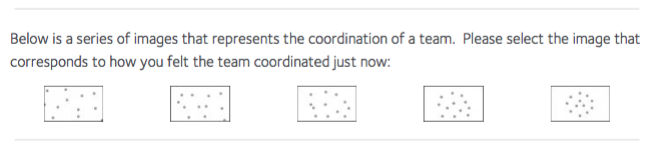
\includegraphics[width = \linewidth]{images/teamClickPictorial.png}
      \caption{Click Pictorial Scale}
      \label{fig:clickPictorial}
    \end{figure}


\myparagraph{\label{app5:bondingPre}Social Bonding}

  \begin{description}
    \item [Emotional Support] ``How emotionally supportive does the team feel?''
    \item [Shared Goal] ``How strong is the feeling that everyone is working towards a shared goal?''
    \item [Group Identification Verbal] A six-item scale designed to measure an individual's personal identification with the stereotypical features of the in-group  \citep{Mael1992}.  All 6 items were measured using a 5-point Likert scale.
          \begin{enumerate}
            \item When someone critises my team, it feels like a personal insult
            \item I am very interested in what others think about my team
            \item When I talk about my team, I usually say ``we'' rather than ``they''
            \item This team's successes are my successes
            \item When someone praises my team, it feels like a personal compliment
            \item If a story in the media criticises my team, I would feel embarrassed
          \end{enumerate}

  \item [Identity Fusion Verbal] A seven-item scale designed to measure an individual's ``feeling of oneness with the group'' \citep{Swann2009}.  Identity Fusion is differentiated from Group Identification in its ability to account for an individual's felt, emotional and personal agentic associations with being a member of the target in-group \citep{Swann2012a}.  All 7 items were measured using a 5-point Likert scale.
    \begin{enumerate}
      \item I am one with my team
      \item I feel immersed in my team
      \item I have a deep emotional bond with my team
      \item My team is me
      \item I’ll do for my team more than any of the other team members would do
      \item I am strong because of my team
      \item I make my team strong
    \end{enumerate}
  \item [Identity Fusion Pictorial] A visual scale designed to measure Identity Fusion to the target in-group \citep{Swann2009}. The pictorial scale depicts two circles, one smaller circle to denote the individual, and one larger circle to denote the group, progressively moving closer to each other such that the most ``fused'' option depicts the smaller circle encased by the larger circle. The scale offers a total of five options to chose from, see Figure ~\ref{fig:fusionPictorialGroup}.  A total of three pictorial scales were included, each with different target in-groups: team, family, and country (China).
  \item [Fusion Pictorial Rank] Athletes were asked to rank their fusion to team, family, and country \citep{Whitehouse2014}.  ``Thinking about these relationships [to team, family, and country] please rank them below in order of which you feel most connected to. 1 for most connected, 3 for least connected.''
  \end{description}


  \begin{figure}[htbp]
    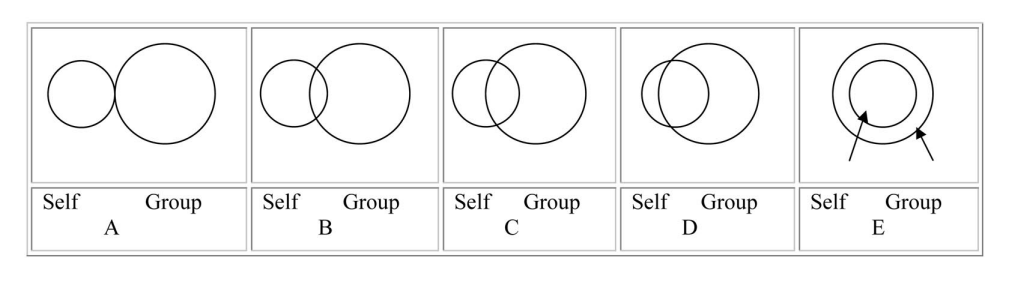
\includegraphics[width=\linewidth]{images/Identity_Fusion_Pictorial_Scale.png}
    \caption{Identity Fusion Pictorial Scale}
    \label{fig:fusionPictorialGroup}
  \end{figure}


\myparagraph{\label{app5:technicalCompetence}Subjective and Objective measures of technical competence}
Athletes were asked about their individual technical competence: ``Rate your individual ability in rugby, relative to: 1) Other teammates currently in your team, 2) Other current professional Chinese rugby players, 3) Professional rugby players form other countries.'' (Items were measured with a zero-centred 100 point scale, -50 - ``Extremely weak'', 0 - ``Average'', 50 - ``Extremely strong'').  Athletes were also asked about perceived competence of their team relative to other Chinese provincial teams: ``Rate your team's overall ability, relative to other teams in China'' (100 point scale, -50 - ``Extremely weak'', 0 - ``Average'', 50 - ``Extremely strong'').  In addition, athletes were asked if their perception of recent performance influences their 1) mood and 2) confidence regarding future performance (All these items were measured with a zero-centred 100 point scale, -50 - ``Extremely weak'', 0 - ``Average'', 50 - ``Extremely strong'').

Athletes were asked to report rugby-related attributes that would provide a more objective indicator of technical competence. These measures included: 1) rugby training age (number of years of experience training for rugby, to the nearest number of years), 2) the number of years spent training with the provincial teams (to the nearest year) , 5) whether the athlete is a usual member of the provincial program's starting team or the reserves.


\myparagraph{\label{app5:TIPI}Ten Item Personality Index}
Athletes were asked to indicate on a 7-point Likert scale the extent to which they agreed with 10 pairs of adjectives as appropriate descriptions of their personality. For example: ``I see myself as: dependable, self-disciplined'' (Response: 1 - ``Disagree strongly'', 2 - ``Disagree moderately'',  3 - ``Disagree a little'', 4 - ``Neither agree nor disagree'', 5 - ``Agree a little'', 6 - ``Agree moderately'', 7 - ``Agree strongly''). In the TIPI, two survey items corresponded to each of the big-five personality types, as follows:

\begin{description}
\item [Extraversion:] 1. Extraverted, enthusiastic; 6. Reserved, quiet (Reversed scale)
\item [Agreeableness:] 2. Critical, quarrelsome (Reversed); 7. Sympathetic, warm
\item [Conscientiousness:] 3. Dependable, self-disciplined; 8. Disorganised, careless (Reversed)
\item [Emotional Stability:] 4. Anxious, easily upset (Reversed); 9. Calm, emotionally stable.
\item [Openness to Experiences:] 5. Open to new experiences, complex; 10.Conventional, uncreative (Reversed)
\end{description}


\myparagraph{\label{app5:teamDisciplinePre}Team Discipline}
Athletes were asked about their feelings regarding their team's commitment to aspects of team discipline over the past month (punctuality to training and team meetings, observing bed times and curfews, attendance at meals, general team conduct) (100 point scale for each item, 0 - ``Extremely poor'', 100 - ``Extremely strong'')).

\myparagraph{Injury Status \label{app5:injuryStatus}}
Athletes responded to a question item asking about their injury status: ``Currently, are you physically able participate in a game?'' (100-point scale (0 = ``Unable to play'', 100 = ``Completely fit to play'').

\myparagraph{Identification Variables\label{app5:IDVariables}}
Athletes reported their date of birth, team affiliation, usual playing position (forward or back), contract and athlete status,




\subsubsection{\label{app5:surveyMid}Mid-Tournament Survey Items}

\myparagraph{\label{app5:performMid}Performance Items}
\begin{description}
\item [Individual Performance Expectations]``Overall, how do you feel about your individual performance in this game?''
\item [Team Performance Expectations] ``Overall, how do you feel about your team's performance in this game?''
\end{description}
Both items used a zero-centred continuous scale, -50 = ``much worse than expected'', 0 =  ``As expected'', 50 =  ``much better than expected''.

\myparagraph{\label{app5:exertionMid}Arousal, Exertion, and Fatigue}
Following each mid-Tournament survey and in the post-Tournament survey, Athletes were asked to report on various components of physical and mental fatigue, exertion, and injury. Athletes were asked about their mood (``How are you feeling now after the tournament?'') and responded by choosing a point on a 10-point scale between three pairs of emotions (``Not aroused / highly aroused'',  ``Depressed/Relaxed'' and  ``Nervous/Excited'').  Athletes were also asked about feelings of fatigue ``How fatigued do you feel as a result of the game/tournament?'', perceived physical exertion (Borg RPE scale, \citep{Borg1990} and perceived mental exertion using two 15-point scales \citep[see][ ]{Noakes2012a}.  Athletes were also asked to indicate their injury status on a 100-point scale (0 = ``Unable to play'', 100 = ``Completely fit to play'').




\subsubsection{\label{app5:surveyPost}Post-Tournament Survey Items}
The post-Tournament survey repeated the mid-Tournament items, asking:
\begin{description}
\item [Individual Performance Expectations] ``Overall, how do you feel about your individual performance during the tournament?''
\item [Team Performance Expectations]``Overall, how do you feel about your team's performance during the tournament?''
\end{description}




\subsubsection{\label{app5:objectivePerformance}Objective Performance Measures}

\begin{description}
\item [Final Rank:] A rank was given to each team based on performance in their respective competition (men's and women's). These rank scores were then reversed for the purposes of statistical analysis (1st place in men's Tournament (8 teams) = 8, 2nd place = 7, and so on)
\item [Total Wins - Losses:] A team's total number of losses was subtracted from its total number of wins.  Thus, more successful teams overall had a higher score.
\item [Total Minutes:] Total number of minutes played throughout the Tournament by each individual athlete
\item [Total Points:] Total number of points scored throughout the Tournament by each individual athlete
\item [Starting Team Average] An average measure indicating likelihood of an athlete being selected in the starting team. Each Athlete was awarded 1 point for each game he or she started in the starting team; reserve squad athletes were awarded zero for each game. Each athlete's total was divided by the total number of games that they participated in during the Tournament, including games in which they didn't take the field, to produce an average score for the Tournament.
\end{description}





\section{Results}


\subsection{Descriptive Statistics}

\subsubsection{\label{app5:descriptivesPre}Pre-Tournament Data Descriptives}

\begin{table}[htpb]\caption{Summary Statistics: post-Tournament Technical Competence (objective and subjective)}
\begin{center}
\begin{small} 
\begin{tabular}
{l
r
r
r
r
r
r
r
}

\multicolumn{
7
}{l}{

}
\cr 
 \hline 
Variable  &  
n  & 
mean  & 
sd  & 
min  & 
max  & 
skew  & 
krtss \cr 

 \hline 

Years In Team   &  120  &   3.17  &   2.12  &    0  &   7  &   0.29  &  -1.25 \cr 

Training Age   &  120  &   4.40  &   2.35  &    0  &  13  &   0.47  &   0.66 \cr 

Starting Team Average   &  172  &   0.61  &   0.36  &    0  &   1  &  -0.43  &  -1.32 \cr 

Age   &  121  &  21.67  &   3.26  &   16  &  32  &   0.52  &  -0.27 \cr 

Ability Teammates   &  120  &  19.45  &  20.14  &  -40  &  50  &  -0.31  &  -0.56 \cr 

Ability Chinese Pros   &  120  &  15.78  &  19.59  &  -35  &  50  &  -0.18  &  -0.65 \cr 

Ability International   &  120  &  18.46  &  26.19  &  -44  &  50  &  -0.48  &  -0.77 \cr 

Team Ability China   &  120  &  22.48  &  22.90  &  -40  &  50  &  -0.64  &  -0.58 \cr 

 \hline 
\end{tabular}
\end{small}
\end{center}
\label{tab:1competenceDescriptives}
\end{table} 




Table ~\ref{tab:1competenceDescriptives} displays the variables relevant to an Athlete's technical competence.  These variables were collected in the pre-Tournament survey, and as such the number of observations per variable is generally 120, except for ``Starting Team Average,'' which was generated from the objective performance data provided by CRFA following the Tournament.  The average number of years in the team was over three years, and the average training age for Athletes was 4.4 years.  In terms of subjective confidence, means for each variable were well above the mid-point of the scale, suggesting that Athletes were on average quite positive about their own ability compared to other athletes (their teammates, other Chinese professionals, International professionals).

\subsubsection{mid-Tournament Data}



\subsubsection{post-Tournament Data}

\begin{table}[htpb]\caption{Summary Statistics: post-Tournament Performance (individual and team)}
\begin{center}
\begin{small} 
\begin{tabular}
{l
r
r
r
r
r
r
r
}

\multicolumn{
7
}{l}{

}
\cr 
 \hline 
Variable  &  
{n} & 
{mean} & 
{sd} & 
{min} & 
{max} & 
{skew} & 
{krtss}\cr 

 \hline 

indPerformance7   &  118  &  56.36  &  23.47  &  0  &  100  &  -0.35  &  -0.08 \cr 

passingTech7   &  118  &  58.41  &  24.25  &  0  &  100  &  -0.79  &   0.05 \cr 

supportAttack7   &  118  &  62.62  &  22.70  &  0  &  100  &  -0.98  &   0.64 \cr 

indDefense7   &  118  &  57.64  &  23.57  &  0  &  100  &  -0.55  &  -0.11 \cr 

effectContact7   &  118  &  62.15  &  24.81  &  0  &  100  &  -0.97  &   0.40 \cr 

decisionAttack7   &  118  &  61.22  &  21.43  &  0  &  100  &  -0.72  &   0.37 \cr 

teamPerformance7   &  118  &  64.36  &  23.61  &  0  &  100  &  -0.52  &  -0.30 \cr 

teamDefense7   &  118  &  62.42  &  22.50  &  0  &  100  &  -0.52  &  -0.52 \cr 

teamAttack7   &  118  &  65.33  &  20.26  &  0  &  100  &  -0.53  &  -0.23 \cr 

teamSupportPlay7   &  118  &  65.75  &  19.72  &  0  &  100  &  -0.76  &   0.57 \cr 

teamCommunication7   &  118  &  65.25  &  21.26  &  0  &  100  &  -0.65  &   0.27 \cr 

 \hline 
\end{tabular}
\end{small}
\end{center}
\label{tab:2performancePostDescriptives}
\end{table} 



\begin{table}[htpb]\caption{Summary Statistics: post-Tournament Team Click}
\begin{center}
\begin{small} 
\begin{tabular}
{l
r
r
r
r
r
r
r
}

\multicolumn{
7
}{l}{

}
\cr 
 \hline 
Variable  &  
{n} & 
{mean} & 
{sd} & 
{min} & 
{max} & 
{skew} & 
{krtss}\cr 

 \hline 

unspokenUnderstanding7   &  118  &  72.72  &  19.95  &  0  &  100  &  -1.38  &  2.13 \cr 

generalAtmosphere7   &  118  &  78.45  &  21.34  &  0  &  100  &  -1.51  &  2.82 \cr 

clickPictorial7   &  118  &   3.93  &   1.04  &  1  &    5  &  -0.78  &  0.00 \cr 

reliabilityOfOthers7   &  118  &  68.00  &  23.09  &  0  &  100  &  -1.33  &  1.75 \cr 

reliabilityForOthers7   &  118  &  63.45  &  25.80  &  0  &  100  &  -1.06  &  0.51 \cr 

abilityExtended7   &  118  &  72.25  &  19.27  &  0  &  100  &  -1.13  &  2.03 \cr 

 \hline 
\end{tabular}
\end{small}
\end{center}
\label{tab:3clickPostDescriptives}
\end{table} 



\begin{table}[htpb]\caption{Summary Statistics: post-Tournament Social Bonding}
\begin{center}
\begin{small} 
\begin{tabular}
{l
r
r
r
r
r
r
r
}

\multicolumn{
7
}{l}{

}
\cr 
 \hline 
Variable  &  
{n} & 
{mean} & 
{sd} & 
{min} & 
{max} & 
{skew} & 
{krtss}\cr 

 \hline 

emotionalSupport7   &  118  &  79.67  &  18.84  &   0.00  &  100  &  -1.74  &  4.37 \cr 

sharedGoal7   &  118  &  86.00  &  15.56  &  29.00  &  100  &  -1.38  &  2.24 \cr 

groupId7   &  118  &   4.29  &   0.67  &   1.50  &    5  &  -1.18  &  1.66 \cr 

fusionVerbal7   &  118  &   4.00  &   0.71  &   1.43  &    5  &  -0.86  &  0.99 \cr 

fusionPictorialTeam7   &  118  &   4.33  &   1.19  &   0.00  &    5  &  -2.45  &  6.07 \cr 

fusionPictorialFamily7   &  118  &   4.51  &   0.96  &   0.00  &    5  &  -2.30  &  5.62 \cr 

fusionPictorialCountry7   &  118  &   4.03  &   1.39  &   0.00  &    5  &  -1.59  &  1.84 \cr 

 \hline 
\end{tabular}
\end{small}
\end{center}
\label{tab:4bondingPostDescriptives}
\end{table} 




\begin{table}[htpb]\caption{Summary Statistics: post-Tournament measures of fatigue}
\begin{center}
\begin{small} 
\begin{tabular}
{l
r
r
r
r
r
r
r
}

\multicolumn{
7
}{l}{

}
\cr 
 \hline 
Variable  &  
n  & 
mean  & 
sd  & 
min  & 
max  & 
skew  & 
krtss \cr 

 \hline 

Fatigue   &  118  &  69.27  &  21.24  &   0  &  100  &  -1.13  &  1.40 \cr 

RPE(physical)   &  118  &  14.97  &   2.66  &   6  &   20  &  -0.80  &  0.49 \cr 

RPE(mental)   &  118  &   6.08  &   2.47  &  -4  &   10  &  -1.13  &  1.82 \cr 

injuryRev7   &  118  &  23.86  &  26.91  &   0  &  100  &   1.19  &  0.60 \cr 

 \hline 
\end{tabular}
\end{small}
\end{center}
\label{tab:5fatiguePostDescriptives}
\end{table} 





\begin{table}[htpb]\caption{Summary Statistics: Objective Tournament Performance}
\begin{center}
\begin{small} 
\begin{tabular}
{l
r
r
r
r
r
r
r
}

\multicolumn{
7
}{l}{

}
\cr 
 \hline 
Variable  &  
n  & 
mean  & 
sd  & 
min  & 
max  & 
skew  & 
krtss \cr 

 \hline 

Final Rank   &  174  &   4.83  &   2.15  &   1  &   8  &  -0.09  &  -1.17 \cr 

Wins - Losses   &  172  &   0.32  &   2.94  &  -6  &   6  &  -0.17  &  -0.25 \cr 

Total Ind Points   &  172  &   8.45  &  11.41  &   0  &  69  &   2.34  &   7.23 \cr 

Total Ind Minutes   &  172  &  44.01  &  20.65  &   1  &  81  &  -0.38  &  -0.89 \cr 

Starting Team Avg   &  172  &   0.61  &   0.36  &   0  &   1  &  -0.43  &  -1.32 \cr 

 \hline 
\end{tabular}
\end{small}
\end{center}
\label{tab:6objectiveTournamentDescriptives}
\end{table} 





Table ~\ref{tab:2performancePostDescriptives} shows that the central tendency for individual and team performance measures was well above the mid-point of the scale, with team performance items slightly higher that individual performance items.  This negatively skewed central tendency in survey responses was more pronounced for variables relating to team click (as Table ~\ref{tab:3clickPostDescriptives} indicates), with the central tendency for each variable ranging between 65 and 78 (100-point scale, SD range = 19-27). The exception to this was the 5-point Team Click Pictorial Scale, the average for which was 3.93 (out of 5, SD = 1.04).  All six items relating to team click had a pronounced negative skew.  As Table ~\ref{tab:4bondingPostDescriptives} demonstrates, the trend for bonding was even higher; central tendencies for Emotional Support and Shared Goal were 79.67 (SD = 18.84) and 86 (SD = 15.56) respectively.  Group Identification Verbal Scale, and Identity Fusion Verbal and Pictorial Scales (5-point Likert) also had a high negatively skewed distribution, with central tendencies between 4 (Identity Fusion Verbal, SD = .71) and 4.51 (Identity Fusion Family, SD = 0.96).
In addition to these main variables of interest, the central tendency of distributions of responses related to arousal, exertion, and fatigue were also well above the mid-point of their respective scales (see Table ~\ref{tab:5fatiguePostDescriptives}).  Table ~\ref{tab:6objectiveTournamentDescriptives} displays athlete objective performance in the Tournament. Athletes played an average of 44 minutes of rugby during the Tournament (just under four full games each), and each Athlete scored an average of 8.45 points, which amounts to between one and two tries each, or a number of try drop-kick conversions (worth two points each).





%<<surveyMeasureSummaryTable, fig.cap =''>>=
%#create all columns:
%Items <- c(IndPerformance, GroupPerformance, TeamPerformance, GroupClick, TeamClick, GroupBonding, TeamBonding, Arousal, Exertion)
%Baseline <- c("*","","*","","*","","*","","")
%Pre <- c("*","*","","*","","*","","*","")
%Post <- c("*","*","","*","*","*","*","*","*")

%surveyMeasureSummary <- data.frame(Variable, Baseline, Pre, Post, stringsAsFactors = FALSE)

%summaryTable <- xtable(surveyMeasureSummary)
%align(summaryTable) <- xalign(summaryTable)
%summaryTable
%@















\begin{enumerate}
  \item A focussed analysis of the \textbf{post-Tournament} survey responses
  \item An analysis of \textit{changes} in variables between \textbf{pre- and post-Tournament} responses
  \item Analysis of the relationship between team performance, team click, and social bonding in survey data over the \textbf{entire Tournament}. \textit{Note that these data are still under analysis and will not be presented for assessment here.}
\end{enumerate}














\section{\label{app5:stats}Statistical Method}

\subsection{\label{app5:EFA}Data Reduction using Exploratory Factor Analysis}
EFA is one of various available data reduction techniques, and is distinct from its main alternative, Principal Components Analysis (PCA), in that it is capable of modelling the latent dimensions of a collection of variables.\footnote{PCA is concerned only with establishing which components exist within the existing data and how a particular variable might contribute that component. To do this, PCA makes the assumption that all variance in a subset of variables is common variance, and therefore communality between all variables is equal to 1. From this assumption, the original data can be transposed into a linear model without the need for a communality-dependent estimated coefficient for each variable \citep{Widaman2007}. EFA examines all the pairwise relationships between individual variables and seeks to extract latent factors from the measured variables.  Squared Multiple Correlations (which are essentially multiple regressions in which each variable is predicted by all others) were used to calculate the common variance (communality) between each variable in an analysis (the communality value is much like an R-squared value from a multiple regression).
The square root of the communality score for each variable is then used as a coefficient that conditions the relationship between each variable and the underlying dimensions (factors) identifiable in the data. Also known as ``factor loadings,'' these coefficients become the parameters of linear model capable of estimating factor scores for each individual observation, which can be utilised in subsequent statistical analysis in place of single variable observations.

A final step in the EFA procedure is the process of ``rotation'', which is an optimisation technique designed to encourage each variable to load on as few factors as possible \citep{Rummel1988}. Rotation refers to a geometric conception of factor analysis, in which individual variables can be plotted in n-dimensional space according to their relationship to each dimension (factor). By rotating the axes of these dimensions, the distance of a given variable to that dimension can be reduced, which results in an increase in factor loading on one factor and (ideally) a decrease in factor loading on another uncorrelated variable. Orthogonal (or perpendicular) rotation of axes refers to axes, say X and Y, maintaining a 90-degree perpendicularity and rotating clockwise or anticlockwise, depending on the location of the variable clusters.
Orthogonal rotation thus enables optimisation of loadings for clusters of variables that are distant from each other in n-dimensional space. If correlation exists between clusters of variables, however, rotating axes obliquely (inwards towards each other) provides a more effective way of reducing the distance between clusters of variables and the latent dimensions that account for such clustering \citep{Osborne2015}. See Figure ~\ref{fig:orthogonalOblique} for a graphical  illustration of the difference between orthogonal and oblique rotation. Given that most variables of interest in the present study were correlated to some degree, I opted for an oblique rotation method \citep{Field2012}. EFAs were conducted using the factanal() function in the Stats package (Version 3.3.0) in R, using the ``promax'' (oblique) rotation method \citep{Gorsuch1983}. Factor scores were calculated as standardised z-scores: zero-centred, with a standard deviation of 1.

\begin{figure}[htbp]
  \begin{center}
    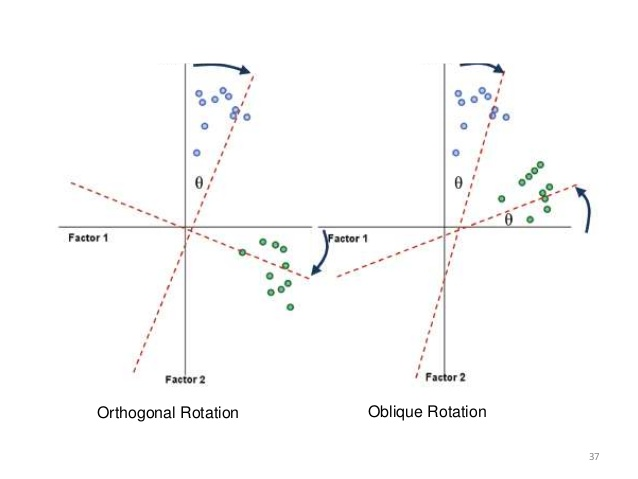
\includegraphics[width= \linewidth, scale = .5]{images/orthogonalObliqueRotationExample.jpg}
    \caption{Orthogonal and oblique rotation methods}
    \label{fig:orthogonalOblique}
  \end{center}
\end{figure}



\subsubsection{\label{app5:samplingAdequacy}Sampling adequacy measures: KMO and Bartlett's Test for Sphericity}

The KMO index provides a proportion measure of common variance to partial correlations among examined variables.  If the KMO index is high ($\approx$ 1), the EFA can act efficiently; if KMO is low ($\approx$ 0), the proposed EFA is not suitable for analysis.

Bartlett’s test of sphericity is used to test the null hypothesis that the correlation matrix is an identity matrix (i.e., a square matrix in which all the elements of the principal diagonal are equal to 1, and all other elements are 0s).

\subsubsection{\label{app5:reliabilityMeasures}Reliability measures: Cronbach's alpha and Guttman's lambda3}


\footnote{Cronbach's $\alpha$ is a function of the number of items in a test, the average covariance between item-pairs, and the variance of the total score \citep{Tabachnick2007}}








\subsection{Data Reduction Summary}


\subsubsection{post-Tournament Data Reduction}

\myparagraph{\label{app5:performanceDataReduction}Team and Individual Components of Performance}
Sampling adequacy measures indicated high suitability ($KMO = 0.83$, $\chi^2(36, N = 118) = 726.60$, $p < .0001$).  As expected, an EFA extracted two factors, with Individual performance measures loaded on one factor (proportion of variance = .34, $SS Loading = 3.09$), and team performance measures loading on a second factor (proportion of variance = .32, $SS Loading = 2.90$). $Guttman's \lambda =.93$ and $Cronbach's \alpha = .90$ indicated that the data reduction was appropriate.





\newpage
\newgeometry{margin=0.5cm} % modify this if you need even more space
\begin{landscape}


% Table created by stargazer v.5.2.2 by Marek Hlavac, Harvard University. E-mail: hlavac at fas.harvard.edu
% Date and time: Mon, Aug 27, 2018 - 18:51:00
\begin{table}[!htbp] \centering 
  \caption{Correlation Matrix: post-Tournament Technical Competence} 
  \label{tab:1competenceCorr} 
\scriptsize 
\begin{tabular}{@{\extracolsep{5pt}} ccccccccc} 
\\[-1.8ex]\hline 
\hline \\[-1.8ex] 
 & Years In Team & Training Age & Starting Team Average & Age & Ability Teammates & Ability Chinese Pros & Ability International & Team Ability China \\ 
\hline \\[-1.8ex] 
Years In Team & $1$ & $0.510$ & $$-$0.044$ & $0.569$ & $0.076$ & $0.102$ & $0.099$ & $0.261$ \\ 
Training Age & $0.510$ & $1$ & $0.0004$ & $0.697$ & $0.095$ & $0.183$ & $0.201$ & $0.190$ \\ 
Starting Team Average & $$-$0.044$ & $0.0004$ & $1$ & $$-$0.040$ & $0.203$ & $0.099$ & $0.044$ & $0.144$ \\ 
Age & $0.569$ & $0.697$ & $$-$0.040$ & $1$ & $0.132$ & $0.089$ & $0.154$ & $0.212$ \\ 
Ability Teammates & $0.076$ & $0.095$ & $0.203$ & $0.132$ & $1$ & $0.428$ & $0.383$ & $0.454$ \\ 
Ability Chinese Pros & $0.102$ & $0.183$ & $0.099$ & $0.089$ & $0.428$ & $1$ & $0.702$ & $0.273$ \\ 
Ability International & $0.099$ & $0.201$ & $0.044$ & $0.154$ & $0.383$ & $0.702$ & $1$ & $0.212$ \\ 
Team Ability China & $0.261$ & $0.190$ & $0.144$ & $0.212$ & $0.454$ & $0.273$ & $0.212$ & $1$ \\ 
\hline \\[-1.8ex] 
\end{tabular} 
\end{table} 


% Table created by stargazer v.5.2 by Marek Hlavac, Harvard University. E-mail: hlavac at fas.harvard.edu
% Date and time: Sun, Jun 25, 2017 - 21:08:16
\begin{table}[!htbp] \centering 
  \caption{Correlation Matrix: post-Tournament Team Performance} 
  \label{tab:22teamPerformancePostCorr} 
\footnotesize 
\begin{tabular}{@{\extracolsep{5pt}} ccccc} 
\\[-1.8ex]\hline 
\hline \\[-1.8ex] 
 & Team Defence & Team Attack & Team Support Play & Team Onfield Communication \\ 
\hline \\[-1.8ex] 
Team Defence & $1$ & $0.834$ & $0.643$ & $0.721$ \\ 
Team Attack & $0.834$ & $1$ & $0.740$ & $0.713$ \\ 
Team Support Play & $0.643$ & $0.740$ & $1$ & $0.715$ \\ 
Team Onfield Communication & $0.721$ & $0.713$ & $0.715$ & $1$ \\ 
\hline \\[-1.8ex] 
\end{tabular} 
\end{table} 


% Table created by stargazer v.5.2 by Marek Hlavac, Harvard University. E-mail: hlavac at fas.harvard.edu
% Date and time: Sun, Jun 25, 2017 - 21:07:58
\begin{table}[!htbp] \centering 
  \caption{Correlation Matrix: Individual Performance} 
  \label{tab:21indPerformancePostCorr} 
\footnotesize 
\begin{tabular}{@{\extracolsep{5pt}} cccccc} 
\\[-1.8ex]\hline 
\hline \\[-1.8ex] 
 & Passing Tech & Support In Attack & Ind Defence & Effectiveness In Contact & Decision Making Attack \\ 
\hline \\[-1.8ex] 
Passing Tech & $1$ & $0.658$ & $0.510$ & $0.508$ & $0.607$ \\ 
Support In Attack & $0.658$ & $1$ & $0.658$ & $0.641$ & $0.734$ \\ 
Ind Defence & $0.510$ & $0.658$ & $1$ & $0.590$ & $0.525$ \\ 
Effectiveness In Contact & $0.508$ & $0.641$ & $0.590$ & $1$ & $0.713$ \\ 
Decision Making Attack & $0.607$ & $0.734$ & $0.525$ & $0.713$ & $1$ \\ 
\hline \\[-1.8ex] 
\end{tabular} 
\end{table} 


% Table created by stargazer v.5.2.2 by Marek Hlavac, Harvard University. E-mail: hlavac at fas.harvard.edu
% Date and time: Mon, Aug 27, 2018 - 18:51:00
\begin{table}[!htbp] \centering 
  \caption{Correlation Matrix: post-Tournament Team Click} 
  \label{} 
\footnotesize 
\begin{tabular}{@{\extracolsep{5pt}} ccccccc} 
\\[-1.8ex]\hline 
\hline \\[-1.8ex] 
 & unspokenUnderstanding7 & generalAtmosphere7 & clickPictorial7 & reliabilityOfOthers7 & reliabilityForOthers7 & abilityExtended7 \\ 
\hline \\[-1.8ex] 
unspokenUnderstanding7 & $1$ & $0.626$ & $0.508$ & $0.275$ & $0.230$ & $0.375$ \\ 
generalAtmosphere7 & $0.626$ & $1$ & $0.385$ & $0.301$ & $0.276$ & $0.265$ \\ 
clickPictorial7 & $0.508$ & $0.385$ & $1$ & $0.282$ & $0.021$ & $0.213$ \\ 
reliabilityOfOthers7 & $0.275$ & $0.301$ & $0.282$ & $1$ & $0.276$ & $0.544$ \\ 
reliabilityForOthers7 & $0.230$ & $0.276$ & $0.021$ & $0.276$ & $1$ & $0.375$ \\ 
abilityExtended7 & $0.375$ & $0.265$ & $0.213$ & $0.544$ & $0.375$ & $1$ \\ 
\hline \\[-1.8ex] 
\end{tabular} 
\end{table} 


\clearpage

% Table created by stargazer v.5.2 by Marek Hlavac, Harvard University. E-mail: hlavac at fas.harvard.edu
% Date and time: Tue, May 30, 2017 - 09:19:43
\begin{table}[!htbp] \centering 
  \caption{Correlation Matrix: post-Tournament Social Bonding} 
  \label{} 
\footnotesize 
\begin{tabular}{@{\extracolsep{5pt}} cccccc} 
\\[-1.8ex]\hline 
\hline \\[-1.8ex] 
 & emotionalSupport & sharedGoal & groupIdentification & identityFusionVerbal & identityFusionPictorialTeam \\ 
\hline \\[-1.8ex] 
emotionalSupport & $1$ & $0.619$ & $0.079$ & $0.331$ & $0.349$ \\ 
sharedGoal & $0.619$ & $1$ & $0.061$ & $0.246$ & $0.395$ \\ 
groupIdentification & $0.079$ & $0.061$ & $1$ & $0.358$ & $0.081$ \\ 
identityFusionVerbal & $0.331$ & $0.246$ & $0.358$ & $1$ & $0.220$ \\ 
identityFusionPictorialTeam & $0.349$ & $0.395$ & $0.081$ & $0.220$ & $1$ \\ 
\hline \\[-1.8ex] 
\end{tabular} 
\end{table} 


% Table created by stargazer v.5.2 by Marek Hlavac, Harvard University. E-mail: hlavac at fas.harvard.edu
% Date and time: Sat, Jun 03, 2017 - 22:22:24
\begin{table}[!htbp] \centering 
  \caption{Correlation Matrix: post-Tournament Fatigue} 
  \label{} 
\footnotesize 
\begin{tabular}{@{\extracolsep{5pt}} ccccc} 
\\[-1.8ex]\hline 
\hline \\[-1.8ex] 
 & fatigue & RPE(physical) & RPE(mental) & injuryRev7 \\ 
\hline \\[-1.8ex] 
fatigue & $1$ & $0.665$ & $0.510$ & $0.090$ \\ 
RPE(physical) & $0.665$ & $1$ & $0.523$ & $0.009$ \\ 
RPE(mental) & $0.510$ & $0.523$ & $1$ & $$-$0.040$ \\ 
injuryRev7 & $0.090$ & $0.009$ & $$-$0.040$ & $1$ \\ 
\hline \\[-1.8ex] 
\end{tabular} 
\end{table} 


% Table created by stargazer v.5.2 by Marek Hlavac, Harvard University. E-mail: hlavac at fas.harvard.edu
% Date and time: Tue, May 30, 2017 - 09:19:44
\begin{table}[!htbp] \centering 
  \caption{Tournament Performance Correlation Matrix} 
  \label{} 
\footnotesize 
\begin{tabular}{@{\extracolsep{5pt}} cccccc} 
\\[-1.8ex]\hline 
\hline \\[-1.8ex] 
 & finalRank & totalWins - totalLosses & totalIndPoints & totalMinutesPlayed & startingTeamAvg \\ 
\hline \\[-1.8ex] 
finalRank & $1$ & $0.901$ & $0.381$ & $0.062$ & $0.055$ \\ 
totalWins - totalLosses & $0.901$ & $1$ & $0.428$ & $0.129$ & $0.089$ \\ 
totalIndPoints & $0.381$ & $0.428$ & $1$ & $0.404$ & $0.067$ \\ 
totalMinutesPlayed & $0.062$ & $0.129$ & $0.404$ & $1$ & $$-$0.038$ \\ 
startingTeamAvg & $0.055$ & $0.089$ & $0.067$ & $$-$0.038$ & $1$ \\ 
\hline \\[-1.8ex] 
\end{tabular} 
\end{table} 


\clearpage
\begin{table}[htpb]\caption{Summary Statistics: post-Tournament Factors}
\begin{center}
\begin{scriptsize} 
\begin{tabular}
{l
r
r
r
r
r
r
r
}

\multicolumn{
7
}{l}{

}
\cr 
 \hline 
Variable  &  
n  & 
mean  & 
sd  & 
min  & 
max  & 
skew  & 
krtss \cr 

 \hline 

objCompetence   &  120  &   0.00  &   0.95  &  -1.99  &    2.91  &   0.45  &  -0.23 \cr 

subjCompetence   &  120  &   0.00  &   0.96  &  -2.58  &    1.79  &  -0.16  &  -0.66 \cr 

indPerformExp   &  118  &  56.36  &  23.47  &   0.00  &  100.00  &  -0.35  &  -0.08 \cr 

indPerformSuccess   &  118  &   0.00  &   0.95  &  -2.96  &    1.70  &  -0.85  &   0.60 \cr 

teamPerformanceExpect   &  118  &  64.36  &  23.61  &   0.00  &  100.00  &  -0.52  &  -0.30 \cr 

jointActionSuccess   &  118  &   0.00  &   0.96  &  -3.28  &    1.79  &  -0.49  &  -0.01 \cr 

teamClick   &  118  &   0.00  &   0.90  &  -3.06  &    1.42  &  -1.01  &   1.03 \cr 

socialBonding   &  118  &   0.00  &   0.89  &  -3.08  &    1.08  &  -1.38  &   2.00 \cr 

fatigue   &  118  &   0.00  &   0.91  &  -3.40  &    1.67  &  -1.03  &   1.56 \cr 

 \hline 
\end{tabular}
\end{scriptsize}
\end{center}
\label{tab:postTournamentFactorDescriptives}
\end{table} 




% Table created by stargazer v.5.2.2 by Marek Hlavac, Harvard University. E-mail: hlavac at fas.harvard.edu
% Date and time: Mon, Aug 27, 2018 - 18:51:01
\begin{table}[!htbp] \centering 
  \caption{post-Tournament Factors Correlation Matrix} 
  \label{tab:postTournamentFactorCorr} 
\scriptsize 
\begin{tabular}{@{\extracolsep{5pt}} cccccccccc} 
\\[-1.8ex]\hline 
\hline \\[-1.8ex] 
 & objCompetence & subjCompetence & indPerformExp & indPerformSuccess & teamPerformanceExpect & jointActionSuccess & teamClick & socialBonding & fatigue \\ 
\hline \\[-1.8ex] 
objCompetence & $1$ & $$-$0.146$ & $0.065$ & $0.319$ & $$-$0.128$ & $$-$0.150$ & $0.011$ & $0.017$ & $0.084$ \\ 
subjCompetence & $$-$0.146$ & $1$ & $$-$0.086$ & $0.125$ & $$-$0.067$ & $0.044$ & $0.145$ & $0.195$ & $$-$0.045$ \\ 
indPerformExp & $0.065$ & $$-$0.086$ & $1$ & $0.411$ & $0.454$ & $0.285$ & $0.226$ & $0.180$ & $0.221$ \\ 
indPerformSuccess & $0.319$ & $0.125$ & $0.411$ & $1$ & $0.411$ & $0.490$ & $0.414$ & $0.273$ & $0.245$ \\ 
teamPerformanceExpect & $$-$0.128$ & $$-$0.067$ & $0.454$ & $0.411$ & $1$ & $0.709$ & $0.570$ & $0.314$ & $0.204$ \\ 
jointActionSuccess & $$-$0.150$ & $0.044$ & $0.285$ & $0.490$ & $0.709$ & $1$ & $0.686$ & $0.404$ & $0.202$ \\ 
teamClick & $0.011$ & $0.145$ & $0.226$ & $0.414$ & $0.570$ & $0.686$ & $1$ & $0.674$ & $0.271$ \\ 
socialBonding & $0.017$ & $0.195$ & $0.180$ & $0.273$ & $0.314$ & $0.404$ & $0.674$ & $1$ & $0.199$ \\ 
fatigue & $0.084$ & $$-$0.045$ & $0.221$ & $0.245$ & $0.204$ & $0.202$ & $0.271$ & $0.199$ & $1$ \\ 
\hline \\[-1.8ex] 
\end{tabular} 
\end{table} 



\end{landscape}
\restoregeometry


\subsection{\label{app:moderatorVarsEFA}Data Reduction for moderator variables}

\subsubsection{Fatigue}
\myparagraph{Post-Tournament}
Post-Tournament survey items relating to perceptions of fatigue and exertion were separately analysed for the purposes of data reduction.  Due to difficulty completing questions related to arousal in the online and in-person surveys, mood-related items were excluded from analysis.  In addition, it was clear from correlation values that injury status did not strongly correlate with other items relevant to fatigue and exertion, and was therefore also excluded from subsequent analysis (see Table ~\ref{tab:5fatiguePostCorr}).  The KMO index and Bartlett's test of sphericity indicated that the remaining subset of variables was appropriate for EFA, $KMO =  0.69$, $\chi^2(3, N = 118) = 111.93$, $p < .001$. EFA was performed on 3 remaining items (fatigue, physical perceived exertion, and mental perceived exertion), which imposed one factor labelled ``Fatigue Factor.''  The extracted factor explained 57.8\% of the overall variance (SS Loadings = 1.7, $Guttman's\lambda =.73$ and Cronbach's $\alpha = .80$).

\myparagraph{Pre- to post-Tournament}
Three survey items related to feelings of fatigue (mental, physical exertion, & fatigue - after the first game!)  were collected and subjected to EFA.
Correlations between variables were high (all $r's > .55$, $KMO = .7$, corrtest Bartlett: $\chi^2(3, N = 238) = 382.88$, $p < .001$).  As such, one factor (``Fatigue Pre Post'') was imposed, which explained 66.3\% of the overall variance (SS Loading = 1.99).  $Guttman's \lambda =.8$ and $Cronbach's \alpha = .85$ indicated that the data reduction was appropriate.
%  $\chi^2(0, N = 238) = 0 $, $p < .001$,

\myparagraph{Overall Tournament}
Fatigue items consisted of fatigue, physical exertion and mental exertion. Correlations between variables were high, indicating that imposing one factor was appropriate (all $r's > .62$, $KMO = 0.71$, $\chi^2(3, N = 440) =  677.37, p < .001$).  The factor imposed for fatigue, ``Fatigue Tournament,'' explained 69\% of the variance ($SS Loading = 2.07$) and $Guttman's \lambda =.82$ and Cronbach's $\alpha = .87$) indicated that the data reduction was reliable.



\subsubsection{Technical Competence}
\myparagraph{Post-Tournament}
Eight items relevant to technical competence were analysed in a correlation matrix to assess relatedness (see Table ~\ref{tab:1competenceCorr}). Medium correlations among measures of objective competence (three out of four items correlated at $> .3$) and among measures of subjective competence (all items except for team competence measure correlated at $> .3$) suggested that the data could be explained by two underlying factors. Team Ability Chinese Provinces was dropped from analysis due to low correlation with other competence variables, possibly because the item did not ask about an individual athlete’s competence (it referred instead to an athlete’s opinion of the competence of the team of which they were a member). An examination of the KMO measure of sampling adequacy ($KMO = .67$), and the Bartlett sphericity test indicated that two factors were adequate, $\chi^2(21, N = 120) = 239.71$, $p < .001$. \\

An EFA of technical competence variables revealed that items of interest loaded on two factors. The exception was the variable Starting Reserve, which failed to load on either factor, and was thus dropped from analysis. Measures of objective competence (Years Team, Training Age, and Age) loaded on the first factor, which was labelled ``Objective Competence'' because the measures were all objective markers of an athlete's competence.  Objective Competence explained 26.4\% of the total variance ($SS Loading = 1.85$). The remaining measures of subjective competence (Ability Teammates, Ability Chinese Pros, Ability International Pros) loaded on the remaining factor.  The second factor was labelled ``Subjective Competence'', due to the fact that all measures were the product of subjective self-report.  Subjective competence explained 23.8\% of the variance ($SS Loading = 1.67$). $Guttman's \lambda =.74$ and $Cronbach's \alpha = (.67)$ indicated that the data reduction was appropriate and reliable.

\myparagraph{Pre- to post-Tournament}
NA
\myparagraph{Overall Tournament}
NA

Summary statistics for the factors extracted from the post-Tournament data, and their correlations can be viewed in Appendix ~\ref{app5:tournamentSurvey} Section
 ~\ref{tab:postTournamentFactorDescriptives} and Table ~\ref{tab:postTournamentFactorCorr} respectively.


















\subsection{\label{app5:modelSelection}Model Selection}
Due to the dependencies in the data and missingness throughout, both traditional ANCOVA (analysis of co-variance) models linear mixed-effects regression models (LMER) are capable of incorporating both fixed and random effects into analysis of variance, however ANCOVA designs only allow the intercept (and not the regression slope) to vary according to level-2 variance, whereas LMER can model the variability of both intercept and slope across different groups of the predictor variable \citep{Field2012}. In addition, the ability of LMERs to deal with unbalanced designs (due to missing values) meant that a LMER was the most suitable modelling strategy for the present study



\section{Intra Class Correlation}

For team-level variance, a one-way random effects model was used, in which average within-team variance (Mean Square Within) of the response variable was divided by the average total variance of the response (Mean Square Total) \citep{Field2005a}.  Each athlete is member of one of 15 teams, which are considered to be sampled from a larger pool of potential teams, hence treated as random effects. The ICC is then interpreted as the percentage of total variance accounted for by group-level variables \citep{Wolak2012}.
To statistically account for the unbalanced design of the data, an adjusted sample-size coefficient (k) was calculated using an equation provided by \citep{Lessells1987}.  While there is no firm agreement on what is deemed meaningful within-group variance, an ICC ratio of $>.10-1.00$ with confidence intervals that do not include zero was considered a strong indication of non-random correlation of group-level residuals \citep{Bailey2011}. As Table ~\ref{tab:ICCsummaryTeam} and ~\ref{tab:ICCsummarySex} indicate, small to moderate team-level intra-class correlation of responses exist for factors of Objective Competence, Joint Action Success, Individual Performance Success, and Team Click. ICCs for Social Bonding and Fatigue meanwhile were relatively low (all $r's <.1$). Sex-level ICCs were all relatively low, suggesting that sex-level variation could be ignored in subsequent inferential analyses.\\





\subsubsection{Intra-Class Correlation}
To assess the need for a statistical model capable of accounting for correlation of residuals, dependency in the data a was quantified using a ratio measure comparing within- and between-group variance, known as the intra-class correlation (ICC). Clustering in the data according to team or sex (the separate men's and women's Tournament) was considered.  In addition to an assessment of ICC values, mean differences in variables of interest were assessed. Owing to the large number of grouping variables (team = 15), pairwise t-tests were not an appropriate way to compute team-level mean differences. Missing values in the data also meant that a standard ANOVA test was also not optimal for multiple group mean comparisons.  Instead, linear regressions were used to approximate differences between group-level responses for post-Tournament survey responses.  Team was used as the predictor variable, and factors derived from performance, click, social bonding, and fatigue variables were used as the outcome variables.  Analyses revealed:

\begin{itemize}
  \item Significant team-level differences in perceptions of success in team component performance (Joint Action Success, $F(14, 103) = 5.63, p < .0001, R^2 = 0.36$) and perceptions of success in individual component performance (Individual Performance Success, $F(14, 103) = 3.23, p < .001, R^2 = 0.21$).
  \item Significant team-level differences in perceptions of overall team performance relative to prior expectations (Team Performance Expectations, $F(14, 103) = 5.96, p < .0001, R^2 = 0.37$), but not perceptions of overall individual performance relative to expectations (Individual Performance Expectations, $R^2 = 0.03 F(14, 103) = 1.24, p = .26$).
  \item Significant team-level differences in team click (Team Click, $F(14, 103) = 4.32, p < .0001, R^2 = 0.28$), significant team-level differences in social bonding $F(14, 103) = 1.84, p = .04, R^2 = 0.09$), but team-level variance of fatigue was not significantly different, (fatigue, $F(14, 103) = 1.46, p = .14, R^2 = 0.05$).
\end{itemize}

An analysis of sex-differences revealed:
\begin{itemize}
  \item Significant sex differences in perceptions of success in individual component performance (Individual Performance Success, $F(1, 116) = 8.03, p < .01, R^2 = 0.06$, men scored significantly higher in self-rated success in components of individual performance, $\beta = 0.48, SE = 0.1709, t(116) = 2.835 p < .01$), but not perceptions of team component performance (Joint Action Success, $F(1, 116) = .002, p = .97, R^2 = -0.009$), perceptions of overall team performance relative to prior expectations (Team Performance Expectations, $F(1, 116) = .09, p = .77, R^2 = -0.008$), or perceptions of overall individual performance relative to prior expectations (Individual Performance Expectations, $F(1, 116) = .05, p = .83, R^2 = -0.008 $).
  \item There were also no significant sex differences in team click (Team Click, $F(1, 116) = .43, p = .51, R^2 = -0.005$), or fatigue ($F(1, 116) = 2.35, p = .13, R^2 = .01 $), but there was a significant sex-difference in social bonding ($F(1, 116) 6.01, p = .02, R^2 = .04$).
\end{itemize}


% Table created by stargazer v.5.2 by Marek Hlavac, Harvard University. E-mail: hlavac at fas.harvard.edu
% Date and time: Sun, Jun 25, 2017 - 21:23:24
\begin{table}[!htbp] \centering 
  \caption{Intra-Class Correlations for post-Tournament Factors according to team} 
  \label{tab:ICCsummaryTeam} 
\small 
\begin{tabular}{@{\extracolsep{5pt}} cccccc} 
\\[-1.8ex]\hline 
\hline \\[-1.8ex] 
 & variable & ICC.team & LowerCI.team & UpperCI.team & k.adjusted.team \\ 
\hline \\[-1.8ex] 
1 & subjectiveCompetence & $0.011$ & $$-$0.057$ & $0.185$ & $8.476$ \\ 
2 & objectiveCompetence & $0.356$ & $0.175$ & $0.625$ & $8.476$ \\ 
3 & jointActionSuccess & $0.374$ & $0.190$ & $0.634$ & $7.768$ \\ 
4 & indPerformanceSuccess & $0.223$ & $0.074$ & $0.484$ & $7.768$ \\ 
5 & teamClick & $0.299$ & $0.130$ & $0.564$ & $7.768$ \\ 
6 & socialBonding & $0.098$ & $$-$0.010$ & $0.324$ & $7.768$ \\ 
7 & fatigue & $0.056$ & $$-$0.036$ & $0.261$ & $7.768$ \\ 
\hline \\[-1.8ex] 
\end{tabular} 
\end{table} 


% Table created by stargazer v.5.2 by Marek Hlavac, Harvard University. E-mail: hlavac at fas.harvard.edu
% Date and time: Sun, Jun 25, 2017 - 21:23:23
\begin{table}[!htbp] \centering 
  \caption{Intra-Class Correlations for post-Tournament Factors according to sex} 
  \label{tab:ICCsummarySex} 
\small 
\begin{tabular}{@{\extracolsep{5pt}} cccccc} 
\\[-1.8ex]\hline 
\hline \\[-1.8ex] 
 & variable & ICC.sex & LowerCI.sex & UpperCI.sex & k.adjusted.sex \\ 
\hline \\[-1.8ex] 
1 & subjectiveCompetence & $0.039$ & $$-$0.006$ & $0.983$ & $58.933$ \\ 
2 & objectiveCompetence & $0.092$ & $0.006$ & $0.992$ & $58.933$ \\ 
3 & jointActionSuccess & $$-$0.017$ & $$-$0.017$ & $0.014$ & $58.390$ \\ 
4 & indPerformanceSuccess & $0.108$ & $0.009$ & $0.993$ & $58.390$ \\ 
5 & teamClick & $$-$0.010$ & $$-$0.016$ & $0.881$ & $58.390$ \\ 
6 & socialBonding & $0.079$ & $0.003$ & $0.991$ & $58.390$ \\ 
7 & fatigue & $0.023$ & $$-$0.009$ & $0.976$ & $58.390$ \\ 
\hline \\[-1.8ex] 
\end{tabular} 
\end{table} 












\subsubsection{Mediation Analysis}
The hypothesised path of relationships outlined in predictions above (specifically: Joint Action Success $\rightarrow$ Team Click $\rightarrow$ Social Bonding) suggests the possibility that Joint Action Success exerts its influence on Social Bonding indirectly, via feelings of ``team click.''  A formal mediation analysis can be used to test the prediction that the relationship between perceptions of joint-action success and social bonding is mediated by feelings of team click, by analysing if and how an intervening variable is causally significant to the relationship between a predictor and an outcome variable. A variable is a mediator if it carries the influence of the predictor variable to an outcome variable, if it serves to explain (either partially or fully) the variance in the outcome variable attributable to the predictor. In the case of this analysis, do perceptions of joint-action success have an indirect effect on feelings of social bonding that is transmitted through feelings associated with team click?

\begin{figure}[htbp]
  \begin{center}
    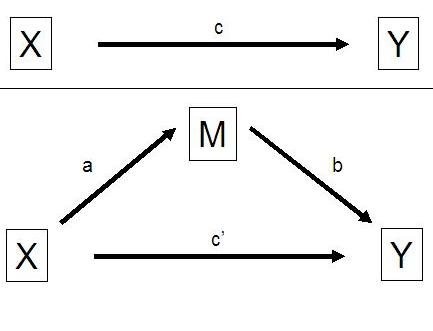
\includegraphics[scale = .5]{images/mediation_image.jpg}
    \caption{Mediation Analysis: direct and indirect effects}
    \label{fig:mediationAnalysis}
  \end{center}
\end{figure}

Mediation analysis works by testing the extent to which the variance in the outcome attributable to a predictor variable (the direct effect, or path ``c'': $Y_i \sim d_Y + cX_i + e_i$) can be explained \textit{indirectly} by the variance of two other relationships: that of the predictor variable and a third mediator (X $\rightarrow$ M, or path ``a'')  and M and the outcome variable (path ``b''), controlling for the direct relationship between X and Y (path ``'c'') (see Figure ~\ref{fig:mediationAnalysis}). The mediation model can thus be denoted by two equations:

\begin{equation}
  M_i \sim d_M + aX_i + e_Mi
\end{equation}

\begin{equation}
  Y_i \sim d_Y + bM_i + c'X_i +  + e_{Yi}
\end{equation}
\bigskip

When combined, these two equations enable the calculation of the ``indirect effect'' of the predictor on the outcome, by controlling for the relationship between the mediator's effect on the outcome variable as a function of its relationship to the predictor variable.  While the direct effect measures the extent to which the dependent variable changes when the independent variable increases by one unit and the mediator variable remains unaltered, the indirect effect measures the extent to which the dependent variable changes when the independent variable is held fixed and the mediator variable changes by the amount it would have changed had the independent variable increased by one unit \citep{Bauer2006}.

The multilevel structure of the data in this study, i.e. the clustering of residuals according to team affiliation, violates the independence assumption of mediation analysis. As such, traditional multiple linear regression and path analysis will produce biased tests of the effects in the mediation model \citep{Raudenbush2002}.
%(Hox, 2002; Kreft & de Leeuw, 1998; Raudenbush & Bryk, 2002).
A multilevel mediation analysis must therefore additionally take into account variance attributable to the random effects of the model (team, in this case), and in so doing capture heterogeneity of variance in the indirect effect due to the level 2 variable \citep{Tofighi2014}.  To do this, each coefficient in the model must be random (denoted by subscript ``j''), so that the value of the coefficient varies across Level 2 units (team): \\

\begin{equation}
  M_{ij} \sim d_{Mj} + a_jX_{ij} + e_{Mij}
\end{equation}

\begin{equation}
  Y_{ij} \sim d_{Yj} + b_jM_{ij} + 'c_jX_{ij} +  + e_{Yij}
\end{equation}
\bigskip

Linear mixed effects regression models are fitted according to these equations, and estimates of mediation effects can be computed from these model parameters.  Subsequent mediation analyses were conducted using the ``mediation'' function of the Causal Mediation Analysis Package (version 4.4.5) in R.






















\section{\label{app5:results}Results}
\subsection{\label{app5:modelRobustness}Model Robustness Checks}


\subsubsection{Prediction 1.a: Joint Action Success predicts Team Click}

BASIC XY RELATIONSHIP? (Post-Tournament Data)

In order to test the prediction that athlete perceptions of joint action are positively related to team click in the post-Tournament data, the following model was constructed:

\begin{equation}
  \begin{align*}
    Team Click =  & Joint Action Success\\
              & + Individual Performance Success \\
              & + Objective Competence + Subjective Competence\\
              & + TournamentPerformanceMeasures \\
  \end{align*}
\end{equation}
\bigskip


\begin{figure}[htbp]
    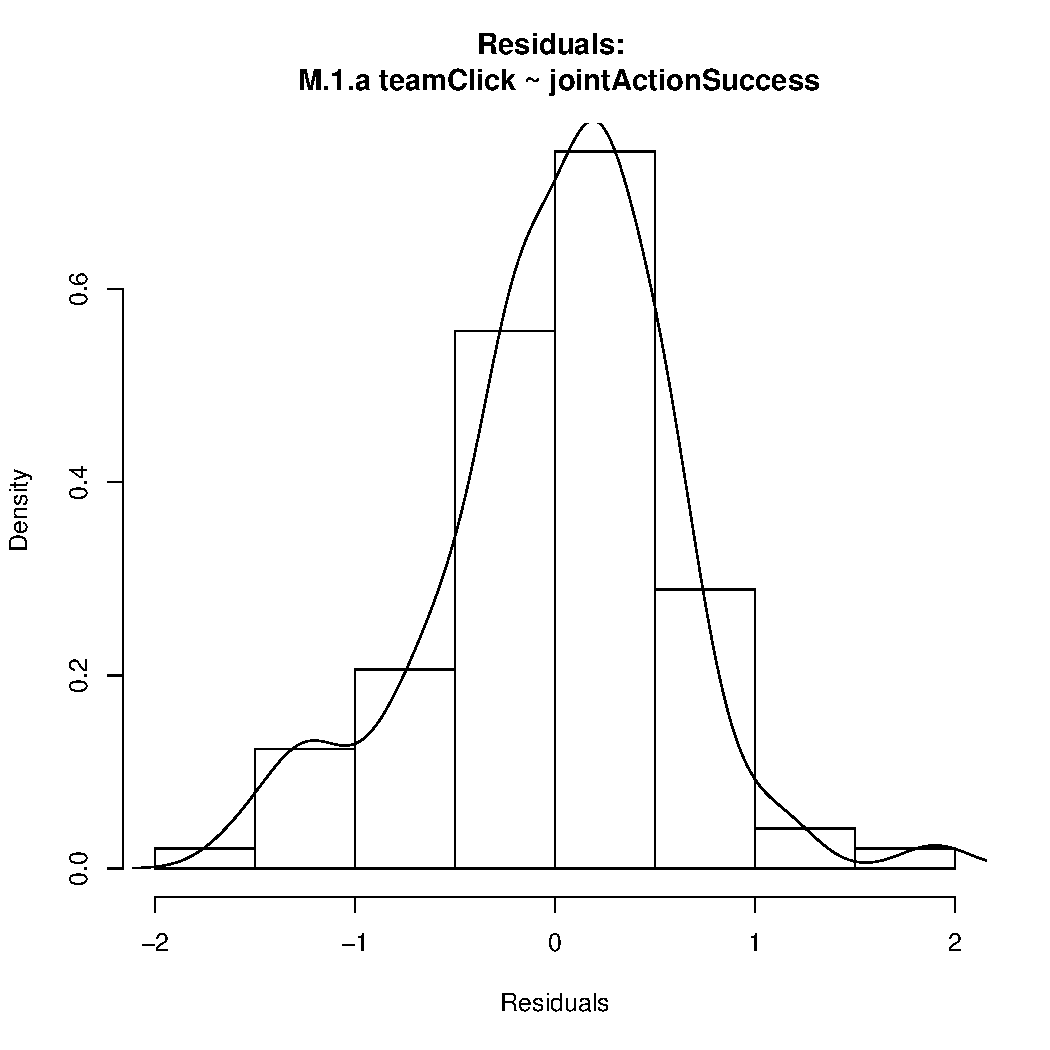
\includegraphics[scale =.4]{images/MLM1aHist.pdf}
    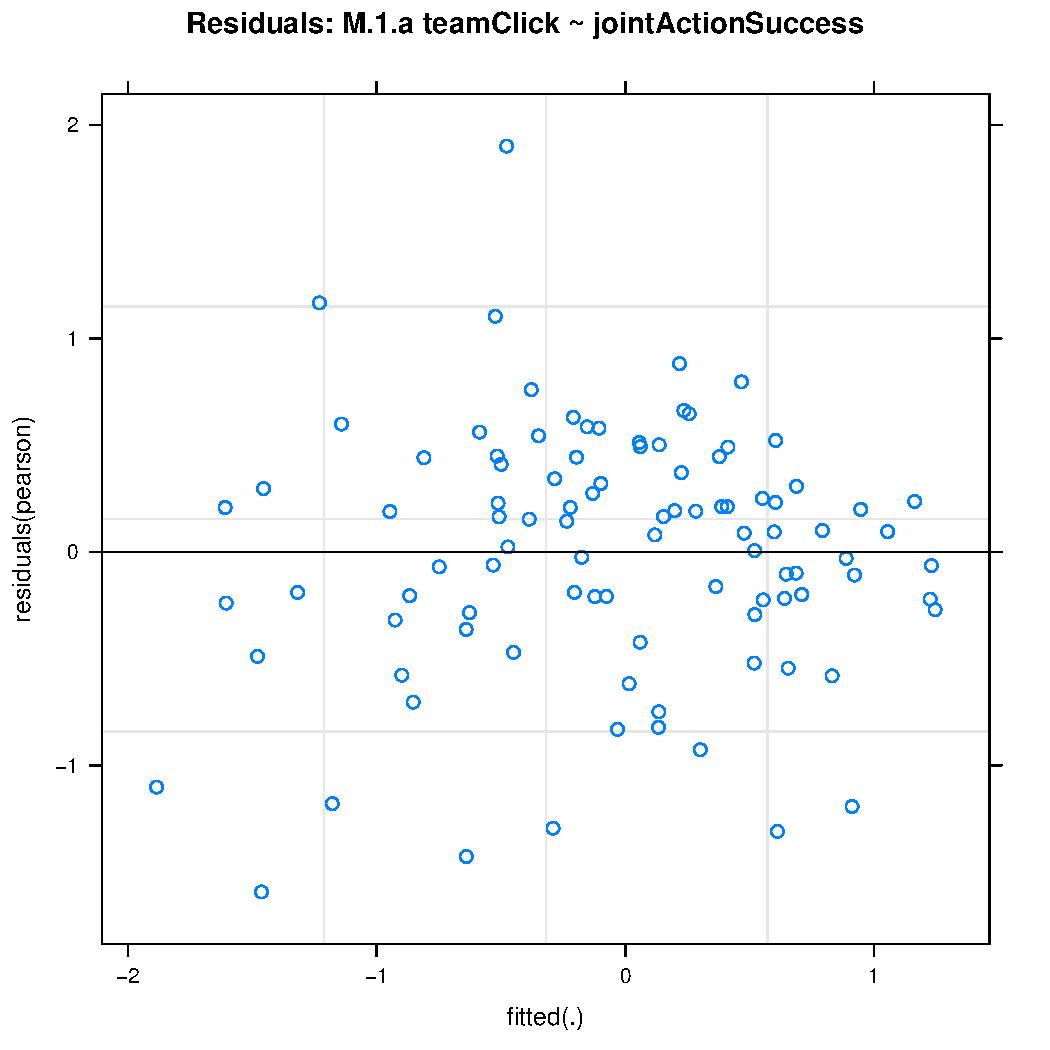
\includegraphics[scale =.4]{images/MLM1aScatter.pdf}
    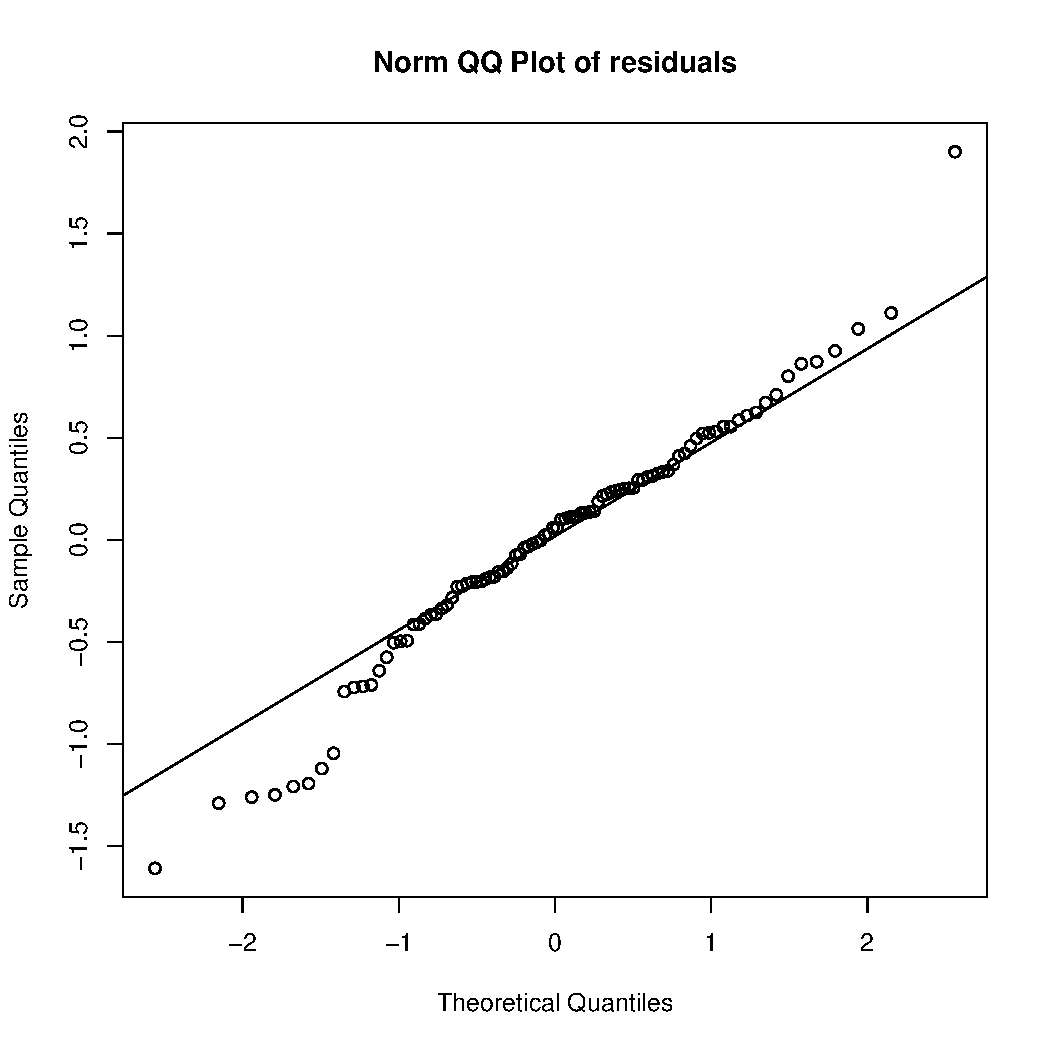
\includegraphics[scale =.4]{images/MLM1aQQPlot.pdf}
    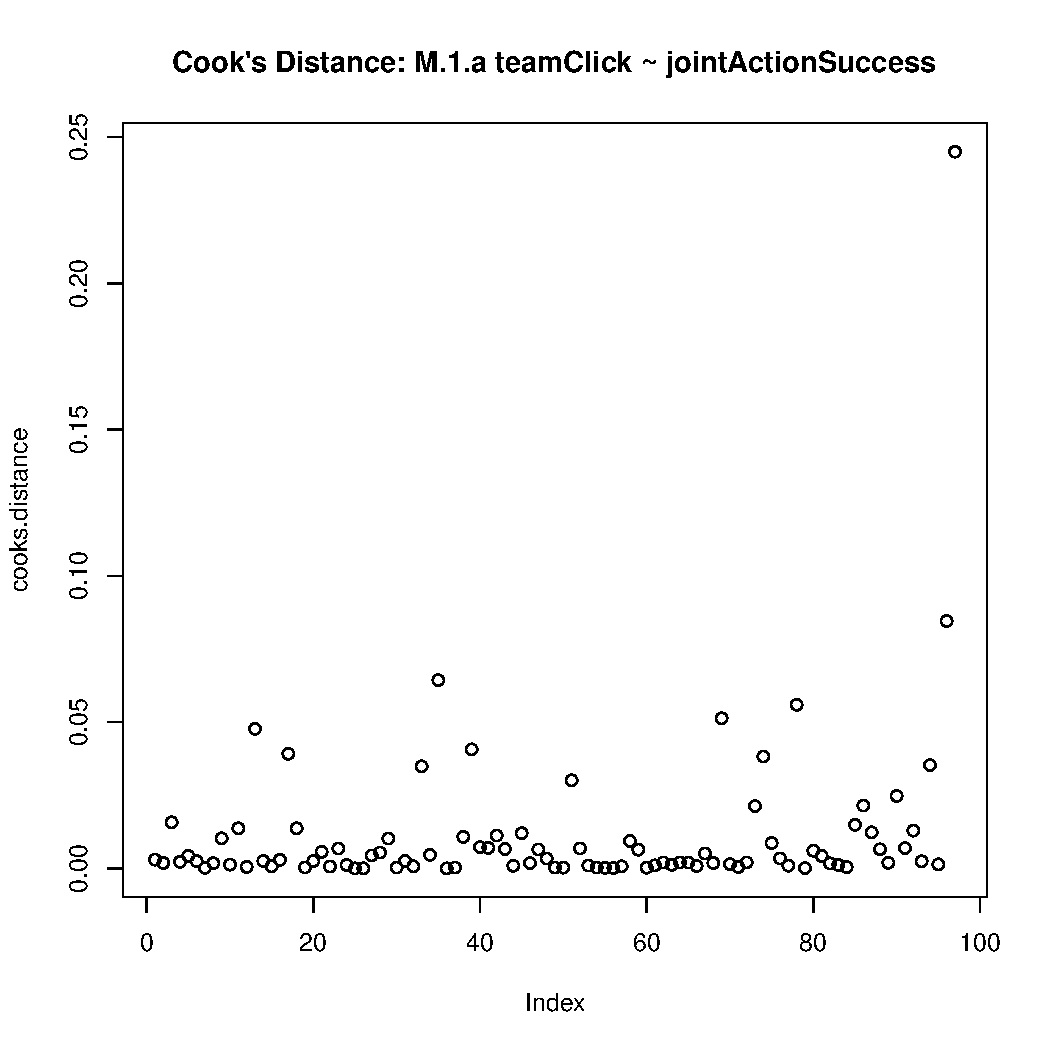
\includegraphics[scale =.4]{images/MLM1aCooksD.pdf}
    \caption{Model Assumptions: 1.a Joint Action Success Predicts Team Click}
    \label{fig:MLM1aAssumptions}
\end{figure}





\begin{figure}[htbp]
  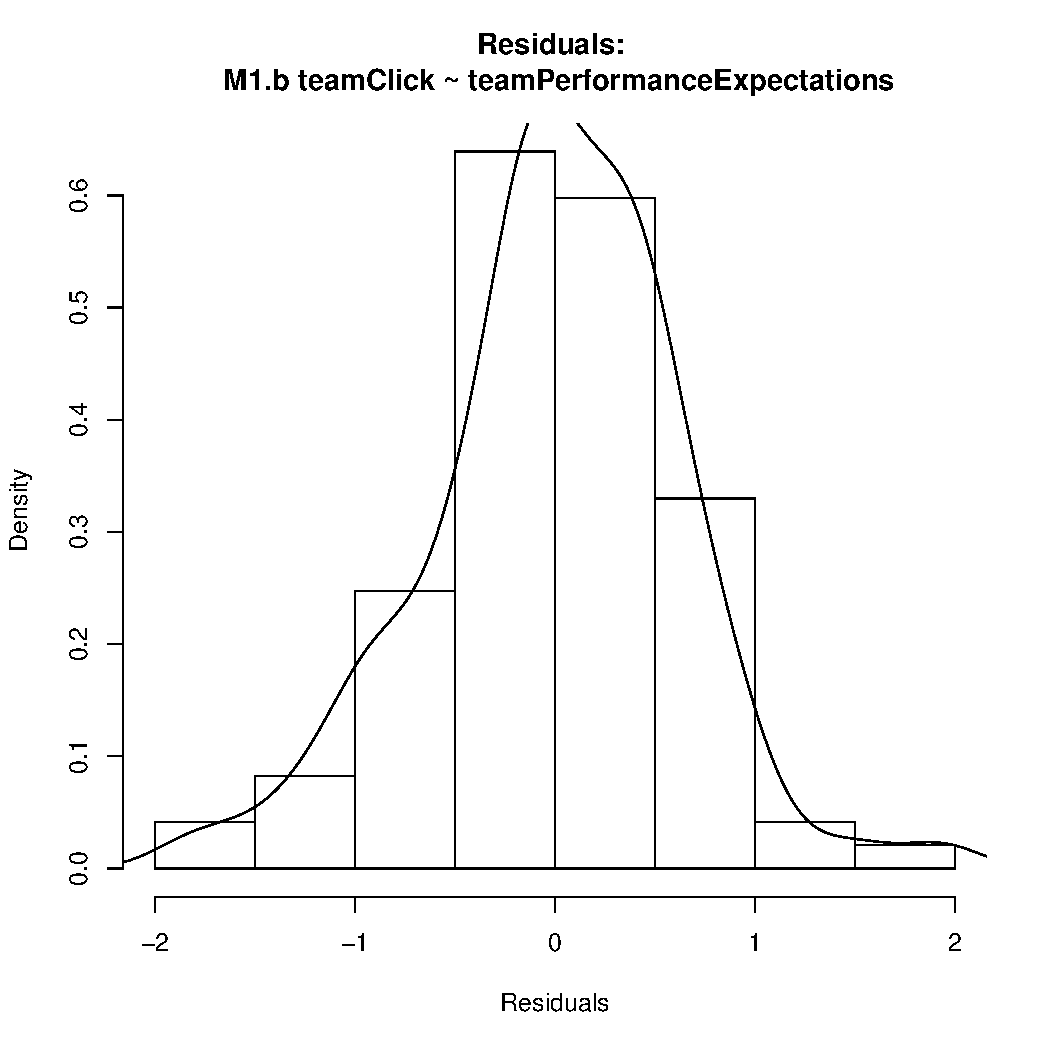
\includegraphics[scale =.4]{images/MLM1bHist.pdf}
  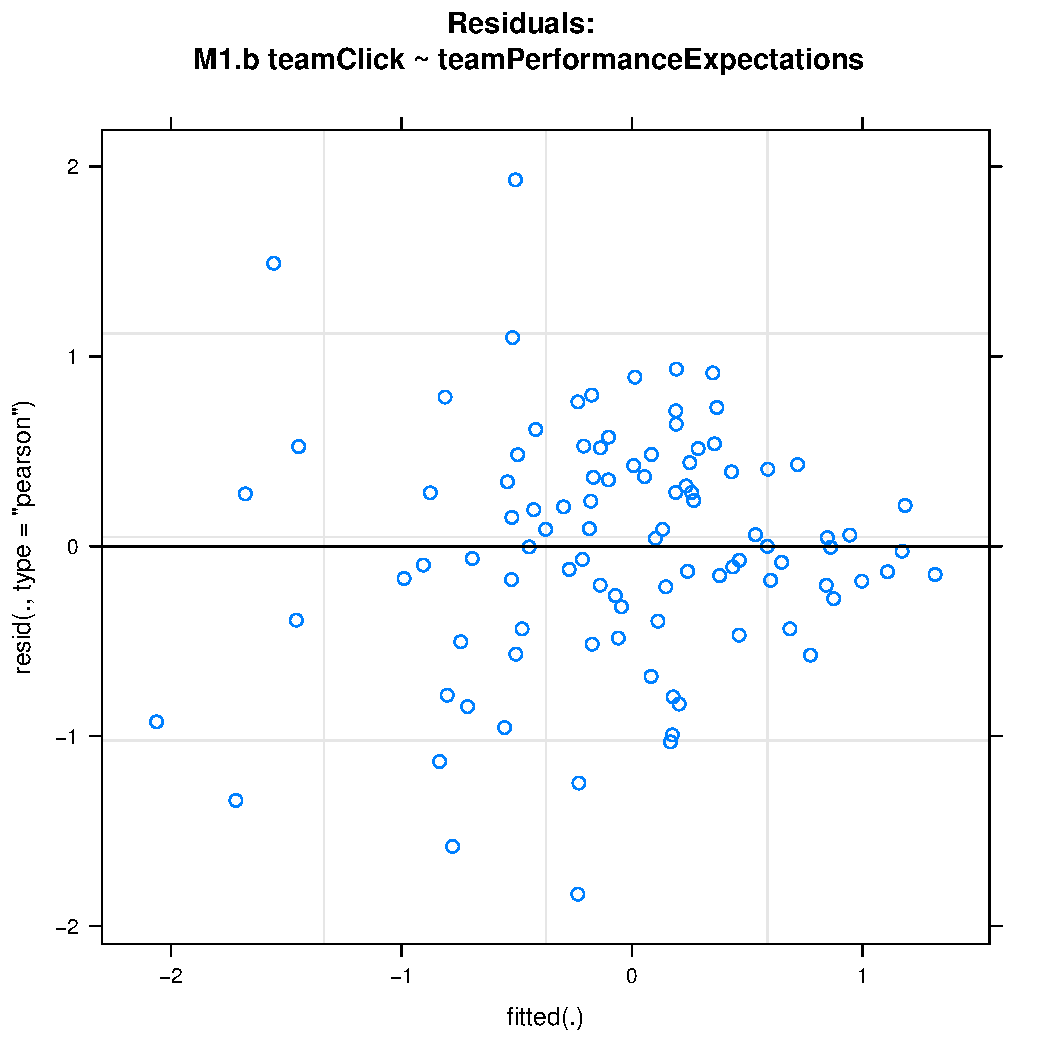
\includegraphics[scale =.4]{images/MLM1bScatter.pdf}
  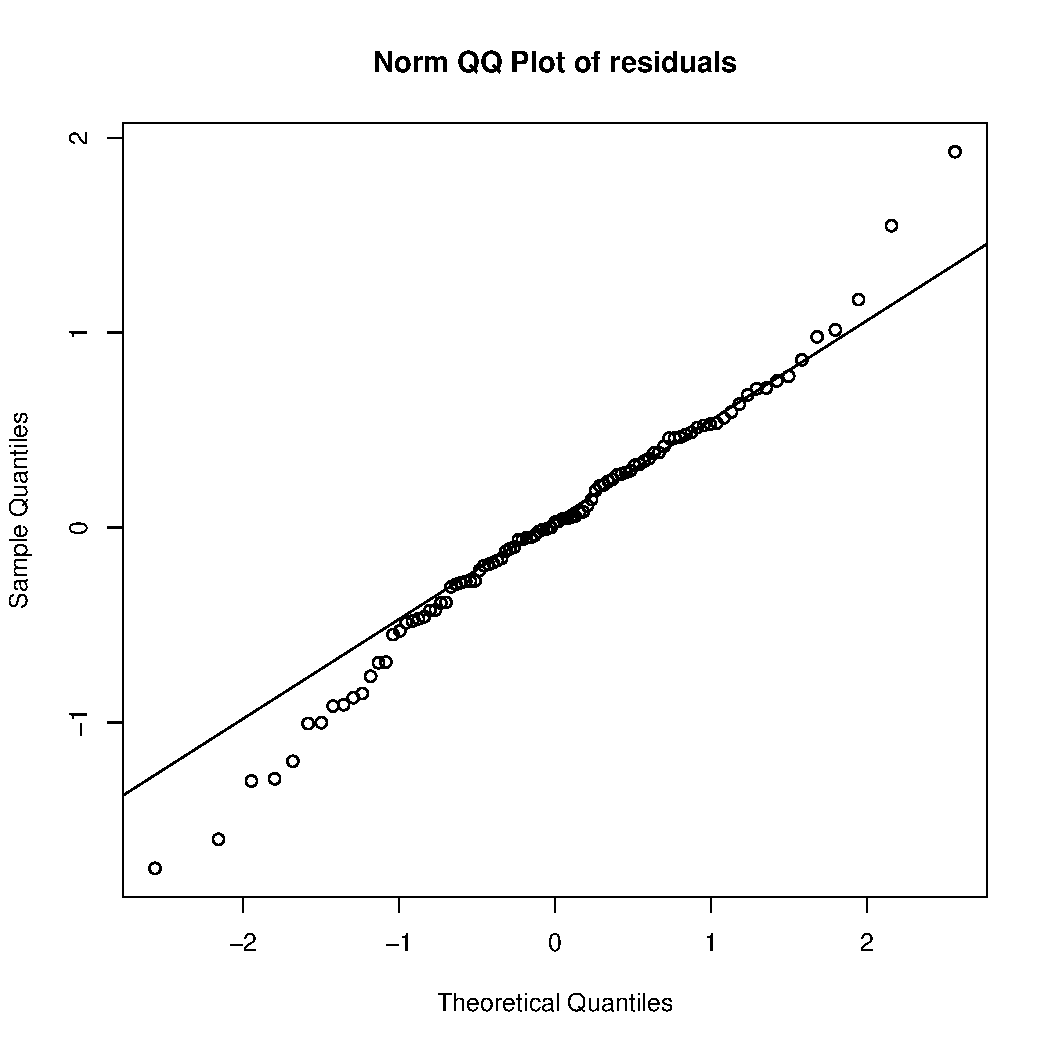
\includegraphics[scale =.4]{images/MLM1bQQNorm.pdf}
  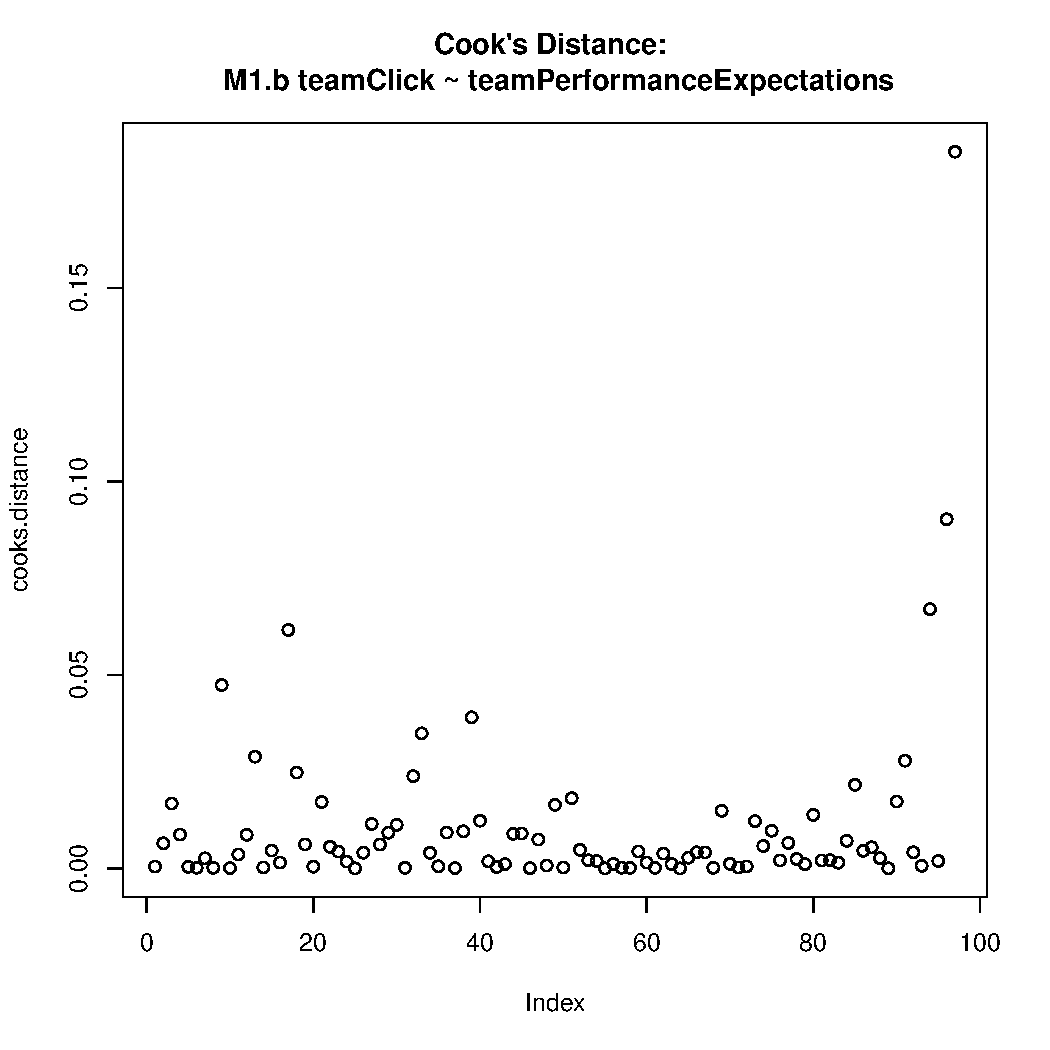
\includegraphics[scale =.4]{images/MLM1bCooksD.pdf}
  \caption{Model Assumptions: Model 1b Team Performance Expectations predict Team Click}
  \label{fig:MLM1bAssumptions}
\end{figure}





% Table created by stargazer v.5.2 by Marek Hlavac, Harvard University. E-mail: hlavac at fas.harvard.edu
% Date and time: Mon, Jun 26, 2017 - 20:35:23
\begin{table}[!htbp] \centering 
  \caption{teamClick = jointActionSuccess X teamPerformanceExpectations} 
  \label{tab:MLM1cPerformanceClickInteraction} 
\footnotesize 
\begin{tabular}{@{\extracolsep{5pt}}lc} 
\\[-1.8ex]\hline 
\hline \\[-1.8ex] 
 & \multicolumn{1}{c}{\textit{Dependent variable:}} \\ 
\cline{2-2} 
\\[-1.8ex] & teamClick \\ 
\hline \\[-1.8ex] 
 (constant) & $-$0.83$^{*}$ \\ 
  & (0.41) \\ 
  & \\ 
 jointActionSuccess & 0.57$^{*}$ \\ 
  & (0.25) \\ 
  & \\ 
 teamPerformanceExpectations & 0.01 \\ 
  & (0.005) \\ 
  & \\ 
 indPerformanceSuccess & 0.01 \\ 
  & (0.10) \\ 
  & \\ 
 indPerformanceExpectations & $-$0.001 \\ 
  & (0.003) \\ 
  & \\ 
 objectiveCompetence & 0.06 \\ 
  & (0.08) \\ 
  & \\ 
 subjectiveCompetence & 0.10 \\ 
  & (0.07) \\ 
  & \\ 
 finalRank & 0.03 \\ 
  & (0.04) \\ 
  & \\ 
 minutesTotal & 0.01 \\ 
  & (0.003) \\ 
  & \\ 
 pointsTotal & 0.004 \\ 
  & (0.01) \\ 
  & \\ 
 teamPerformanceComponentsFactorPost:teamPerformance7 & 0.0001 \\ 
  & (0.003) \\ 
  & \\ 
\hline \\[-1.8ex] 
Marginal R-squared & .56 \\ 
Conditional R-squared & .65 \\ 
Observations & 97 \\ 
Log Likelihood & $-$90.96 \\ 
Akaike Inf. Crit. & 217.91 \\ 
Bayesian Inf. Crit. & 264.26 \\ 
\hline 
\hline \\[-1.8ex] 
\textit{Note:}  & \multicolumn{1}{r}{$^{*}$p$<$0.05; $^{**}$p$<$0.01; $^{***}$p$<$0.001} \\ 
\end{tabular} 
\end{table} 






\begin{figure}[htbp]
  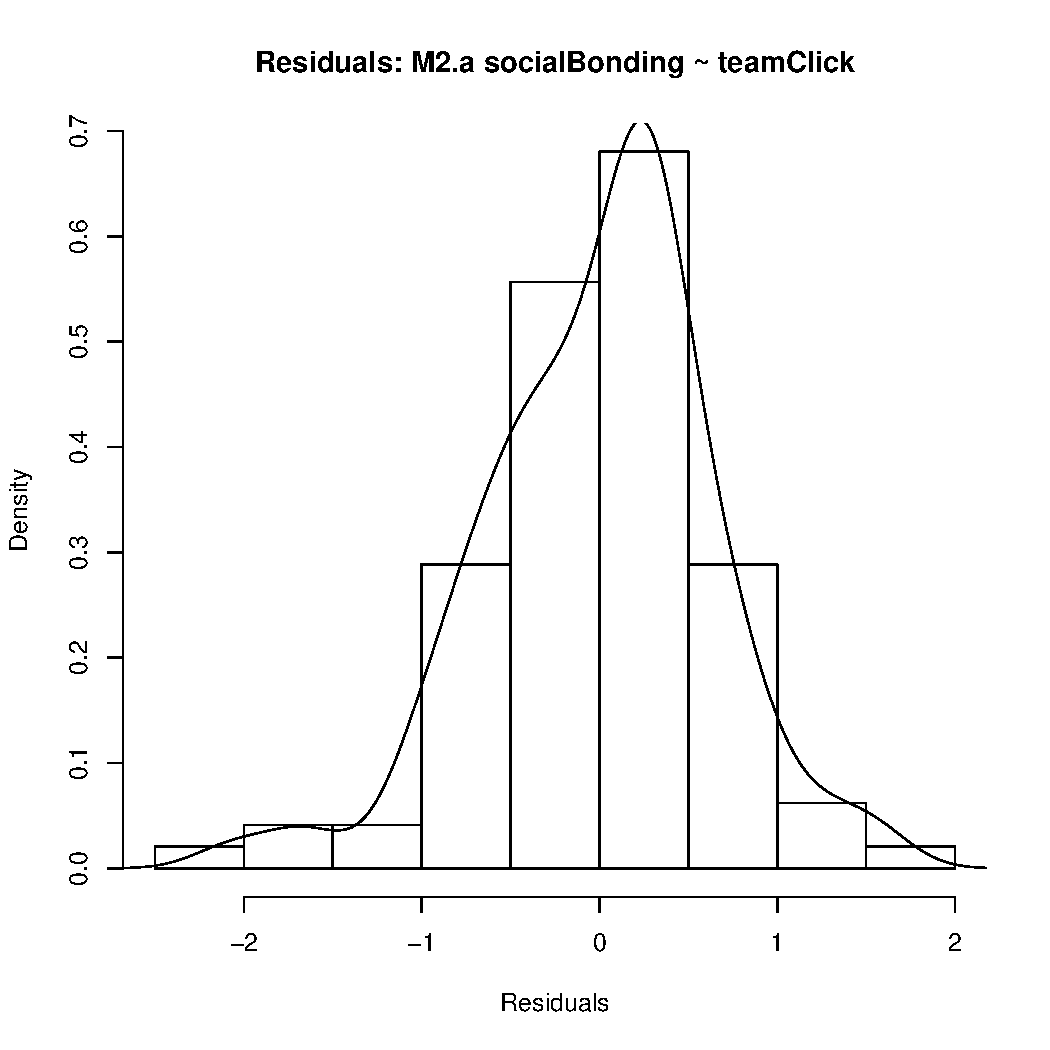
\includegraphics[scale =.4]{images/MLM2aHist.pdf}
  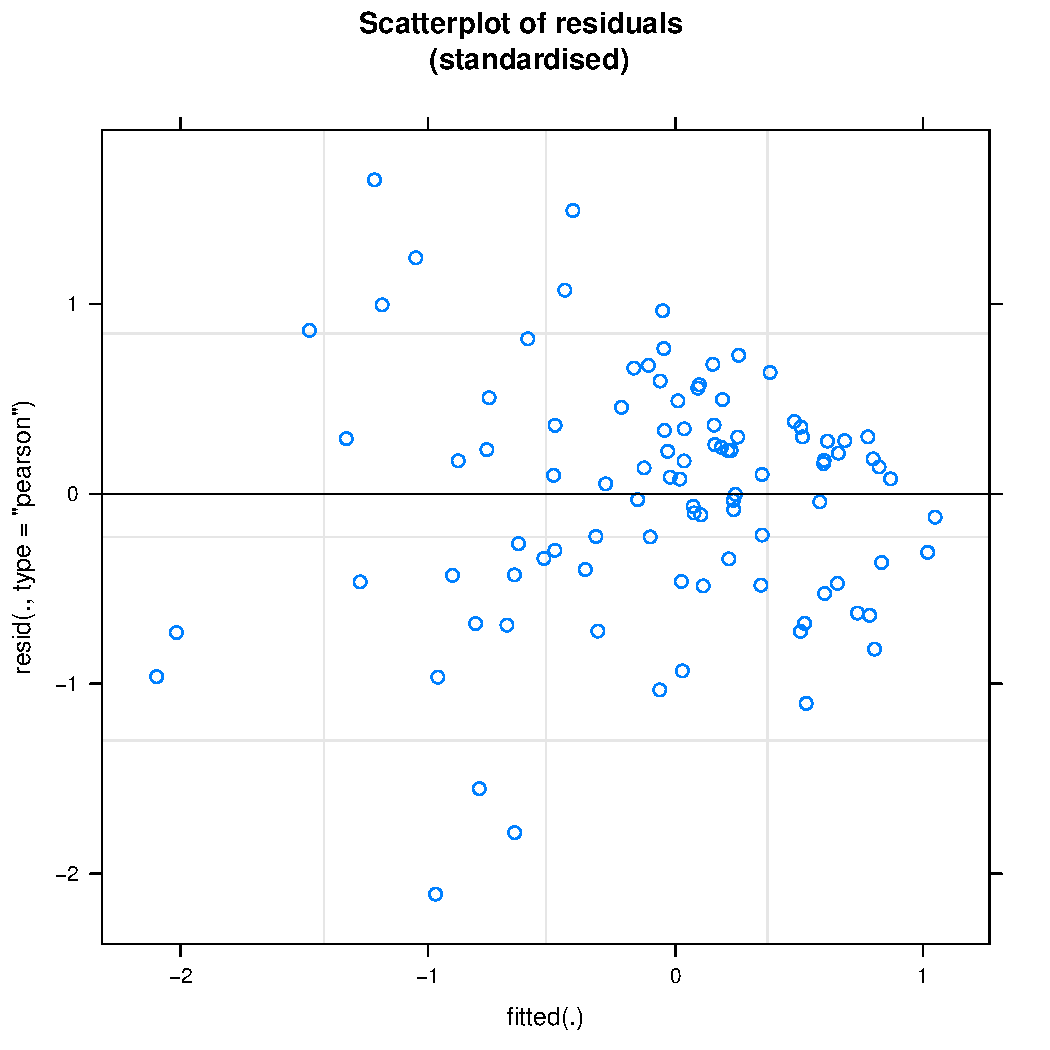
\includegraphics[scale =.4]{images/MLM2aScatter.pdf}
  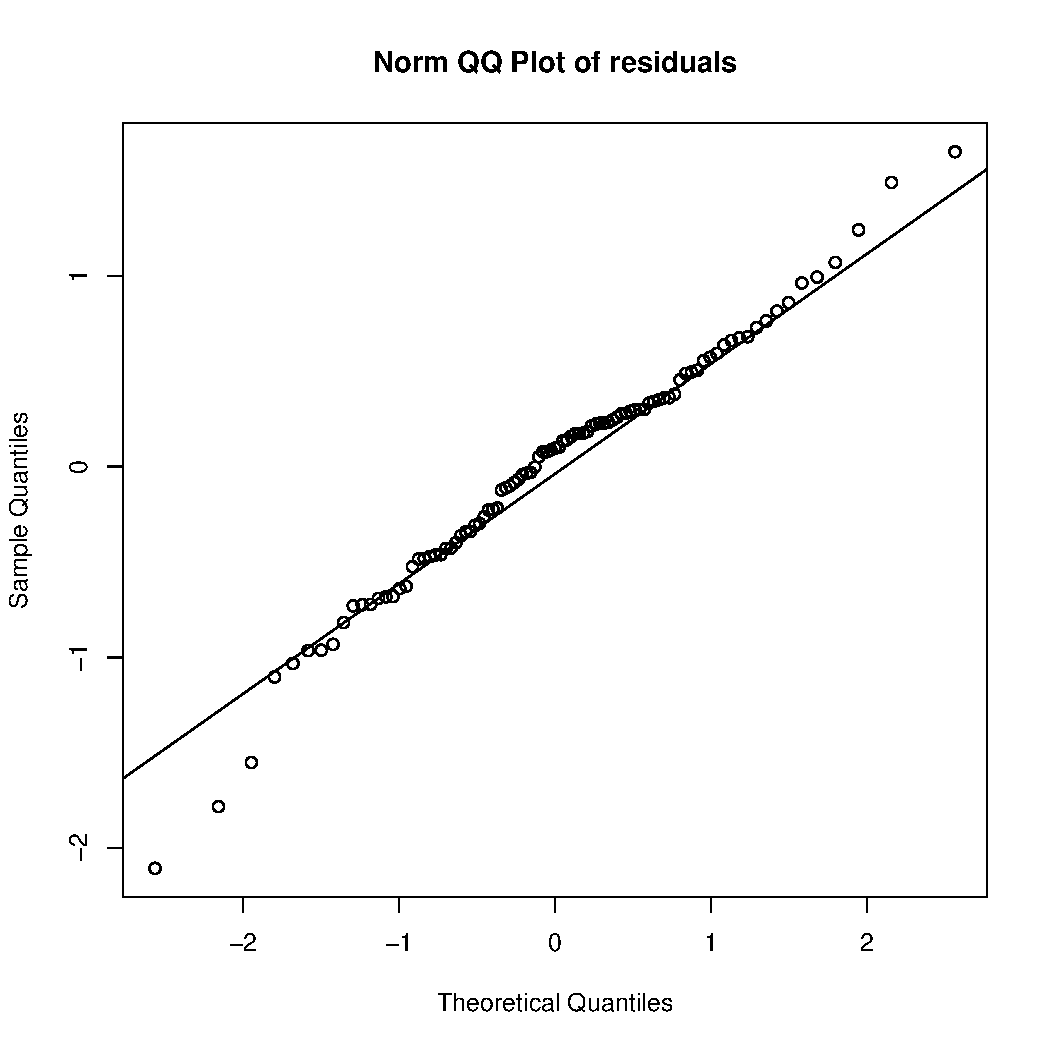
\includegraphics[scale =.4]{images/MLM2aQQNorm.pdf}
  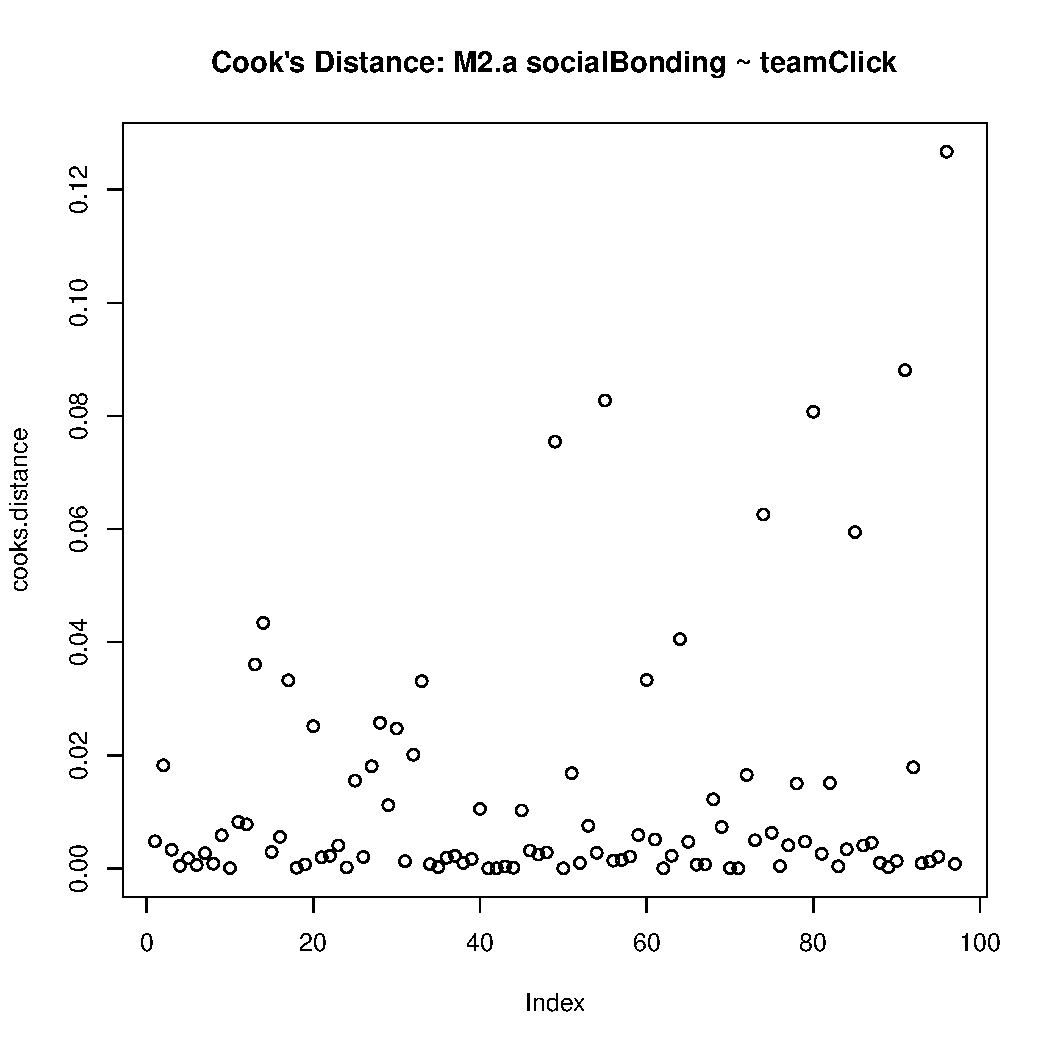
\includegraphics[scale =.4]{images/MLM2aCooksD.pdf}
  \caption{Model Assumptions: M2a Team Click predicts Social Bonding}
  \label{fig:MKM2aAssumptions}
\end{figure}





\begin{figure}[htbp]
  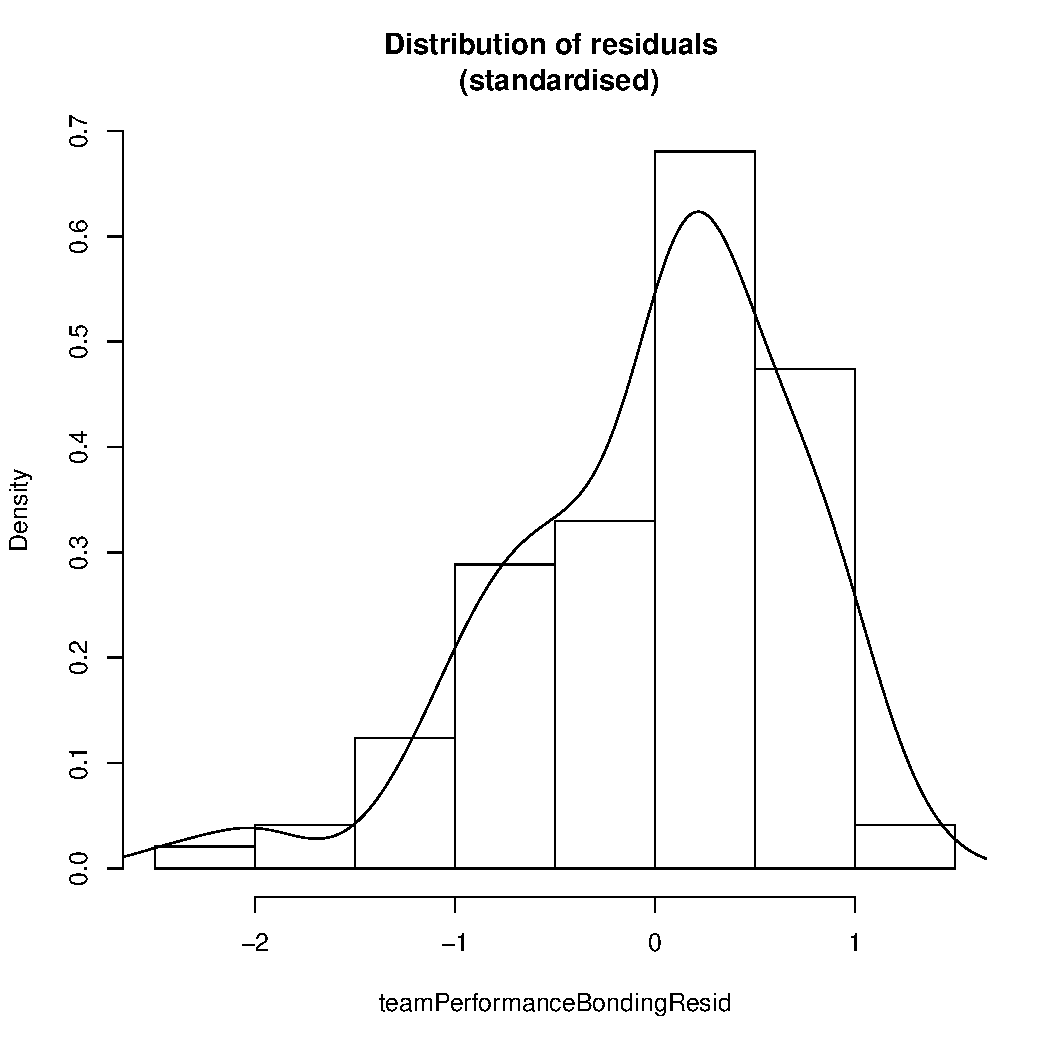
\includegraphics[scale =.4]{images/MLM3aHist.pdf}
  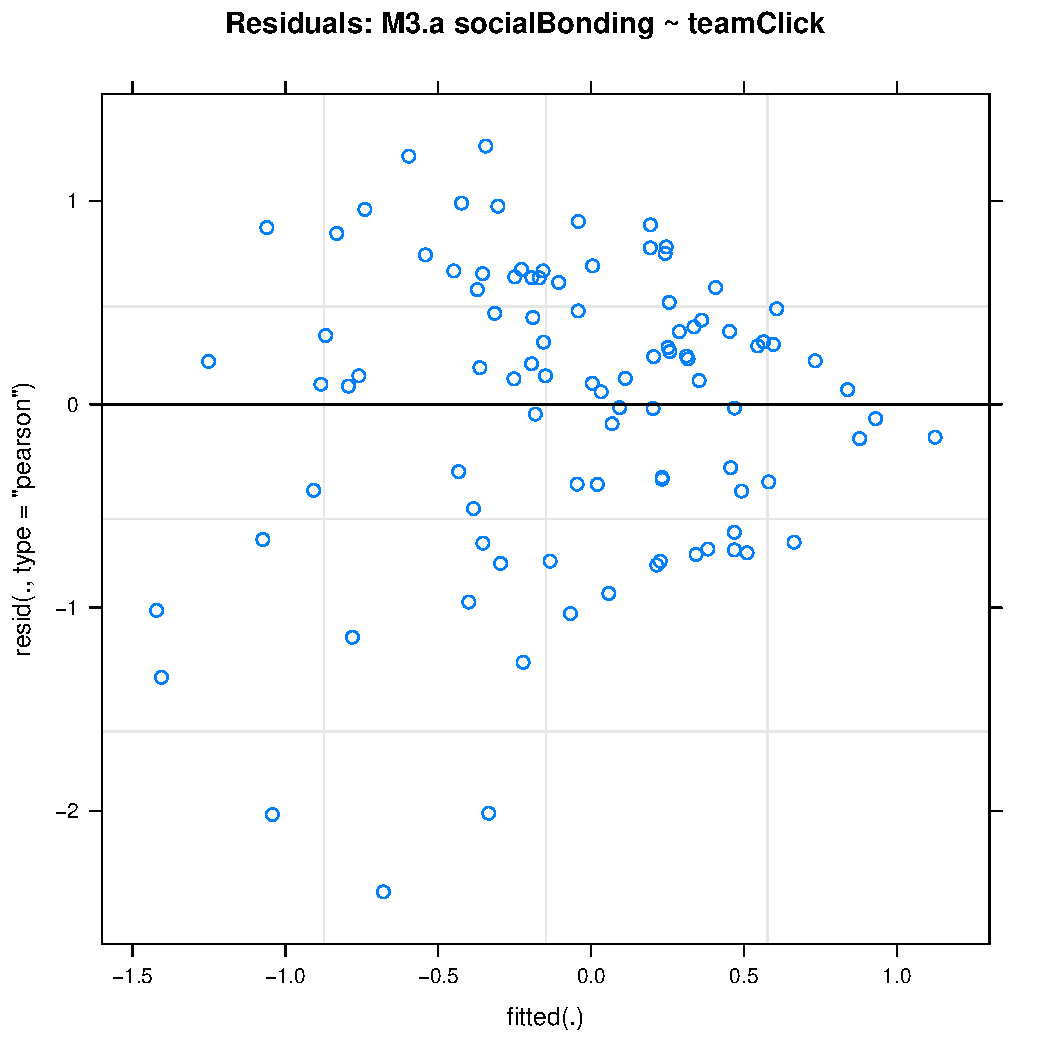
\includegraphics[scale =.4]{images/MLM3aScatter.pdf}
  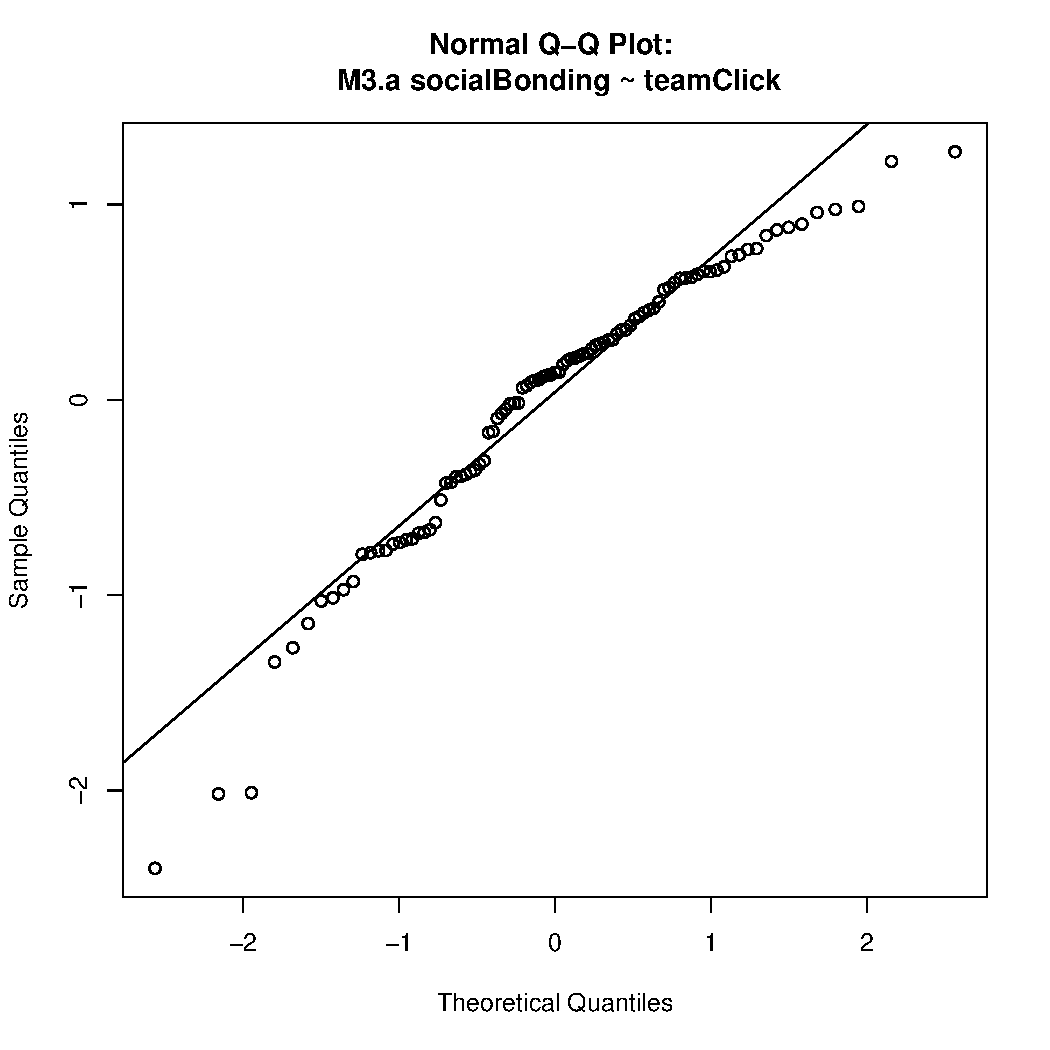
\includegraphics[scale =.4]{images/MLM3aQQNorm.pdf}
  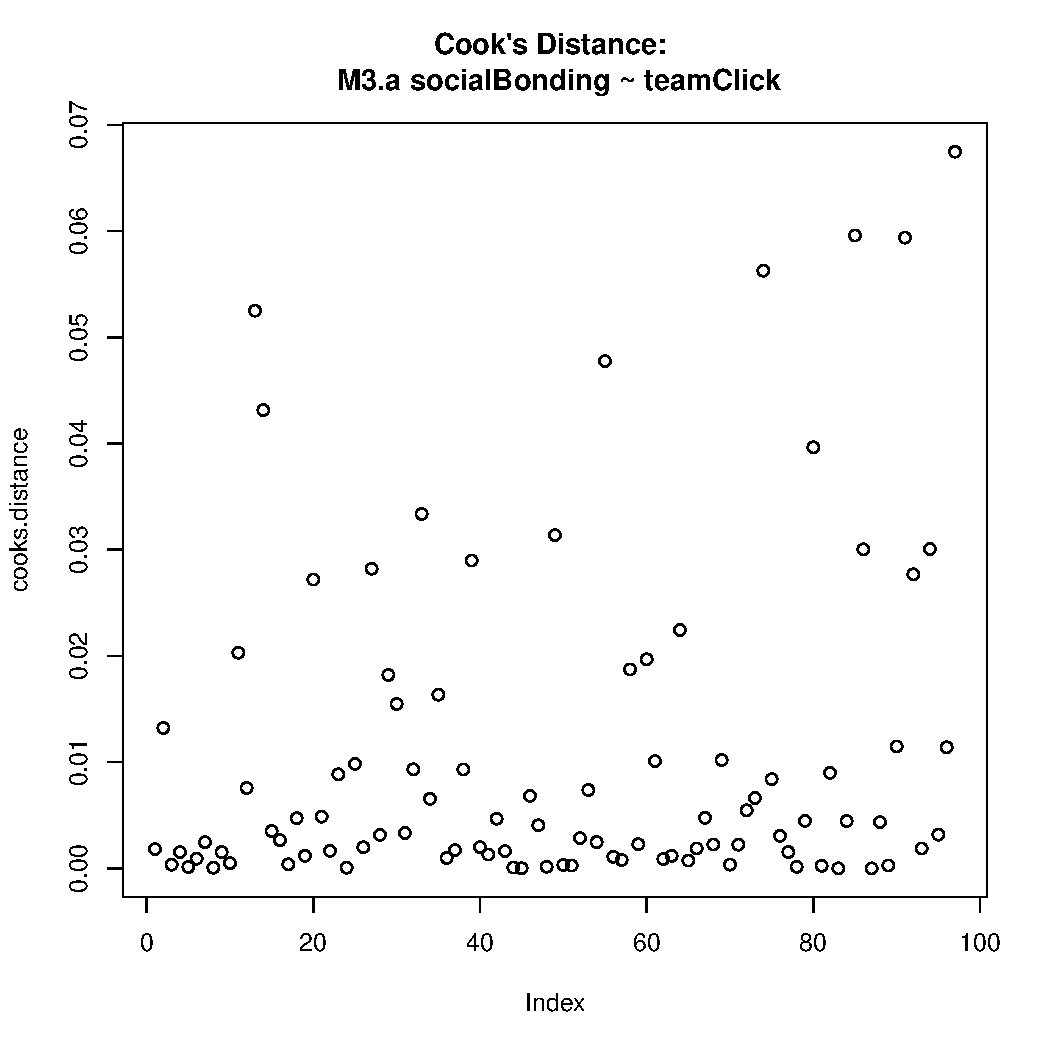
\includegraphics[scale =.4]{images/MLM3aCooksD.pdf}
  \caption{Model Assumptions: M3a Joint Action Success predicts Social Bonding}
  \label{fig:MLM3aAssumptions}
\end{figure}

\begin{figure}[htbp]
  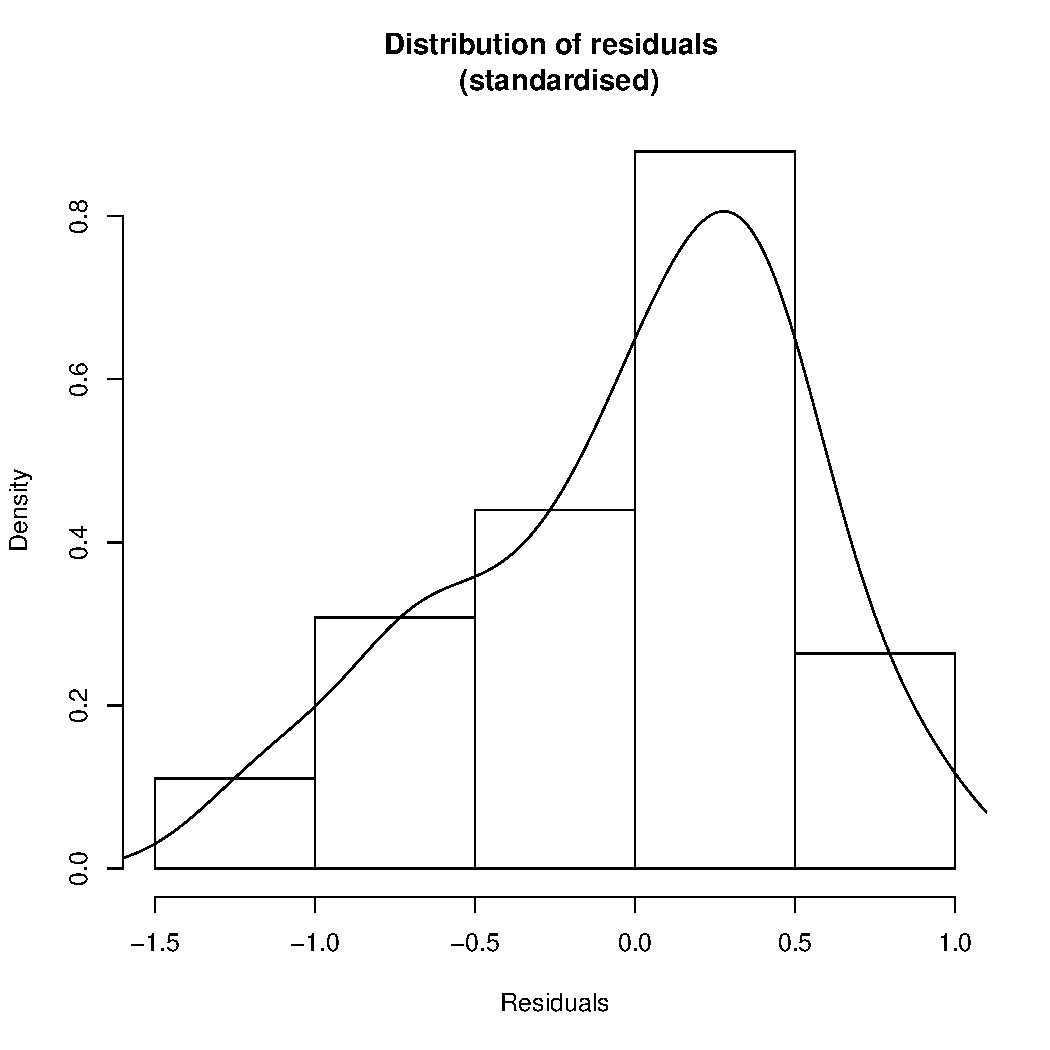
\includegraphics[scale =.4]{images/MLM3aOutHist.pdf}
  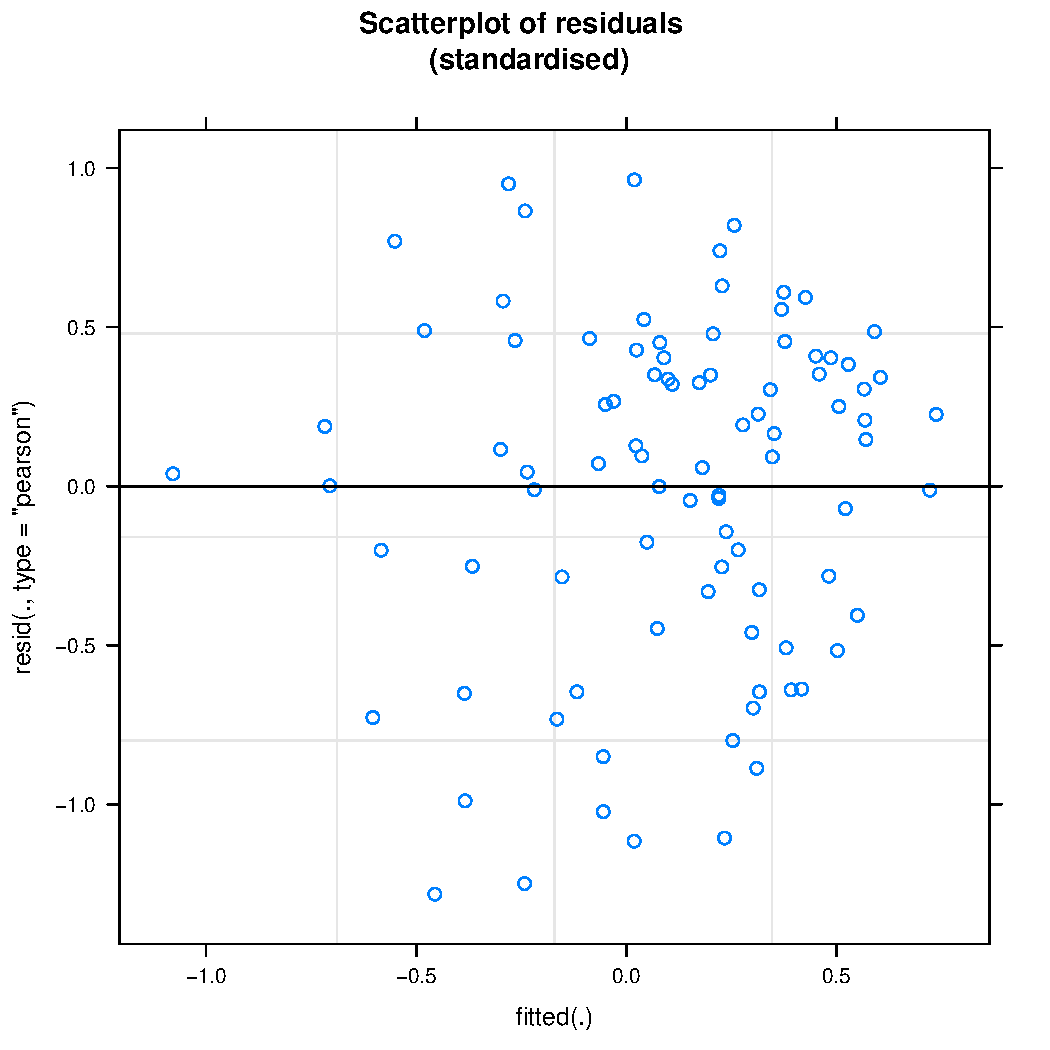
\includegraphics[scale =.4]{images/MLM3aOutScatter.pdf}
  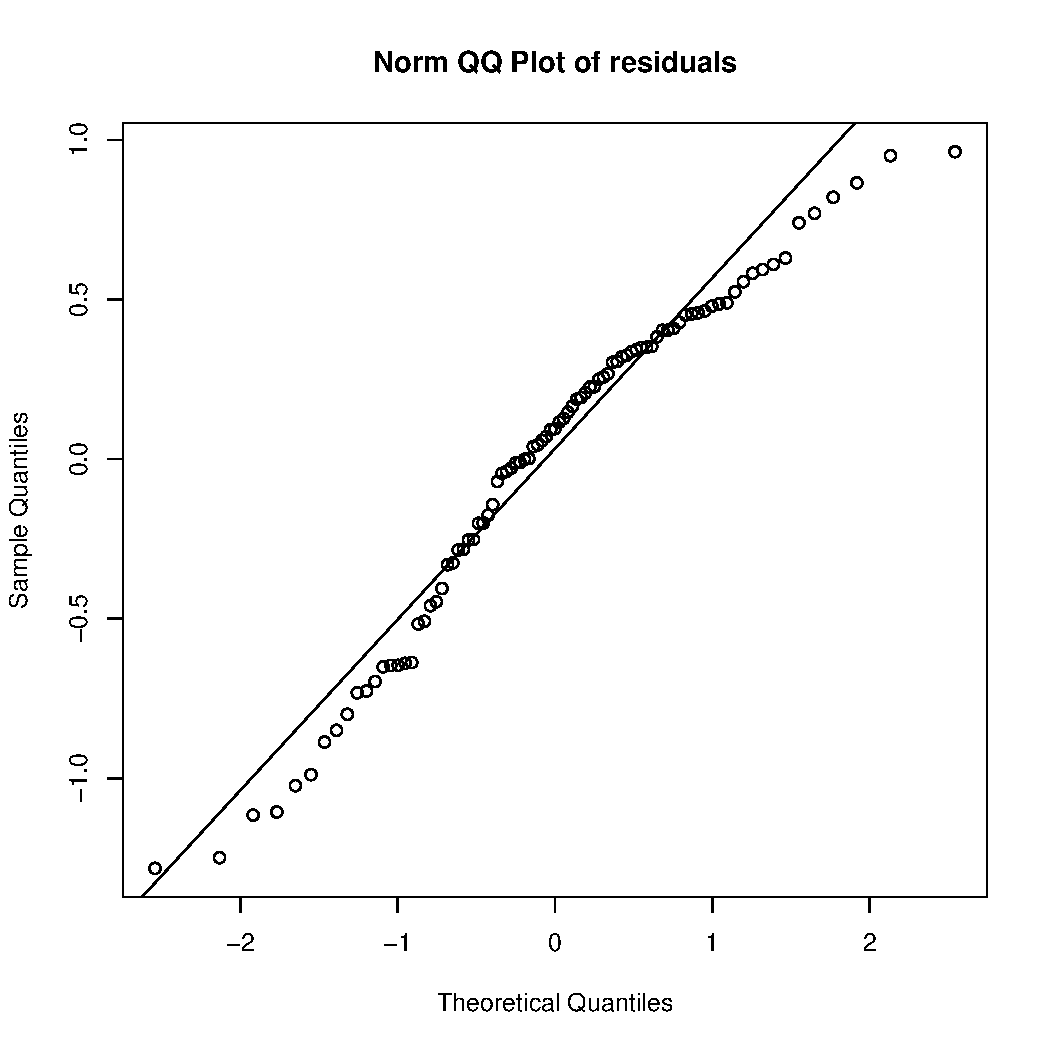
\includegraphics[scale =.4]{images/MLM3aOutQQNorm.pdf}
  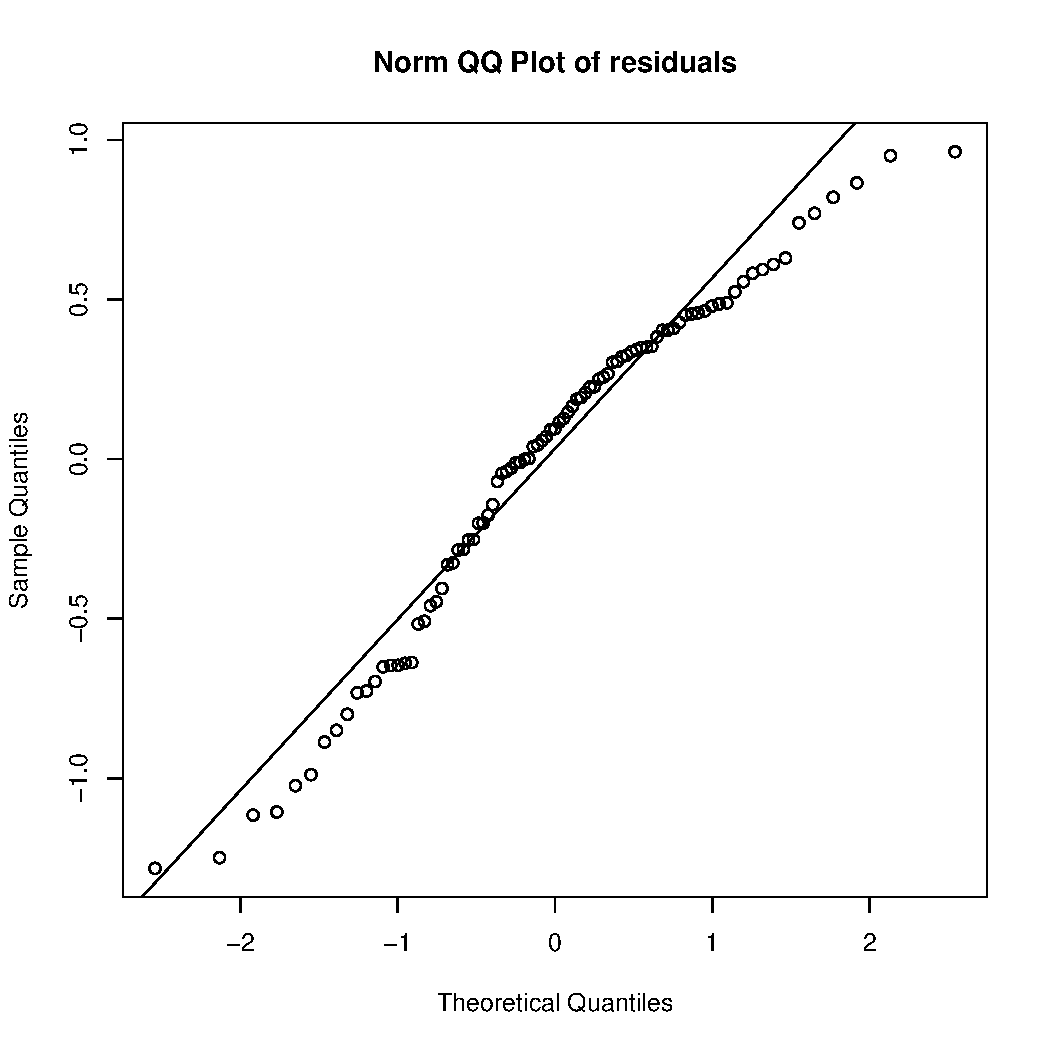
\includegraphics[scale =.4]{images/MLM3aOutCooksD.pdf}
  \caption{Model Assumptions: M3a Joint Action Success predicts Social Bonding (outliers removed)}
  \label{fig:MLM3aOutAssumptions}
\end{figure}

\begin{figure}[htbp]
  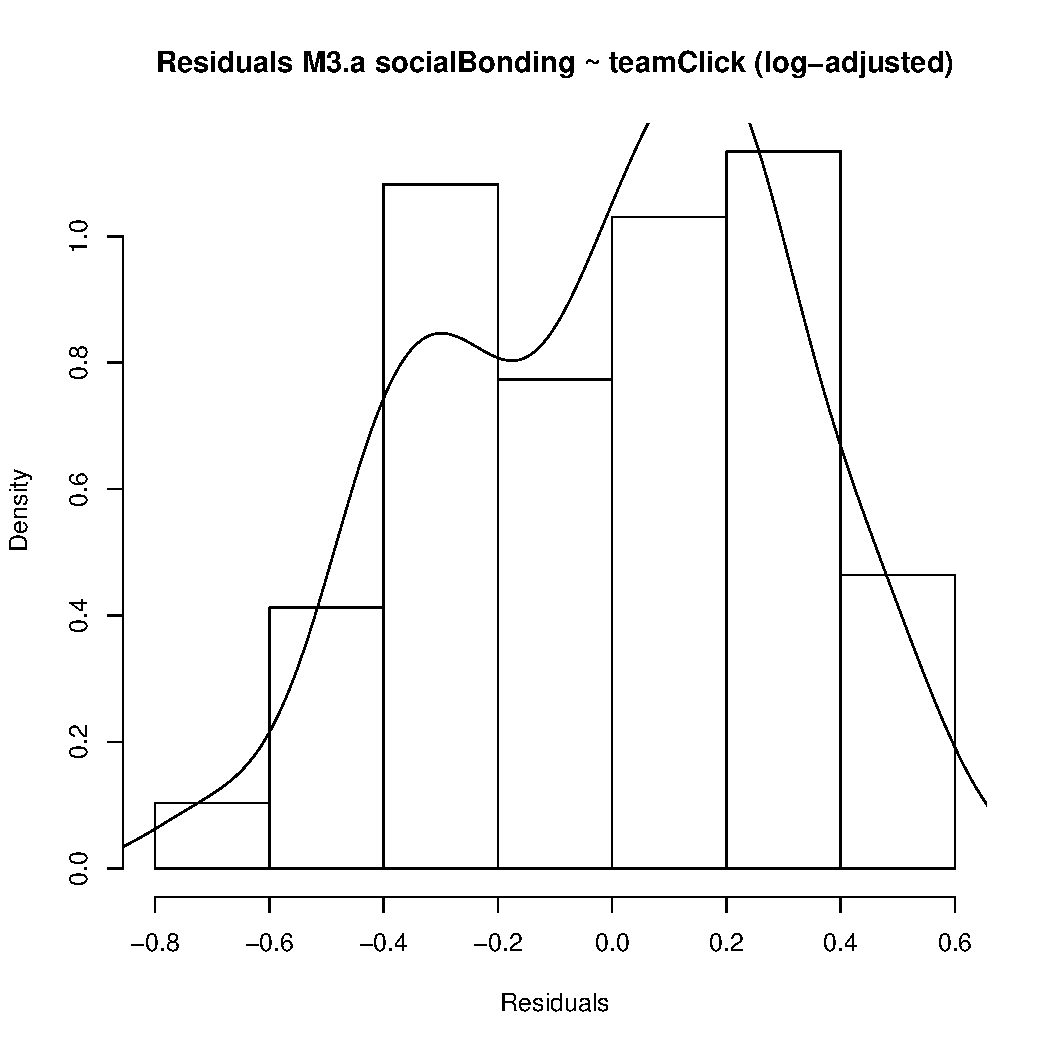
\includegraphics[scale =.4]{images/MLM3aLogHist.pdf}
  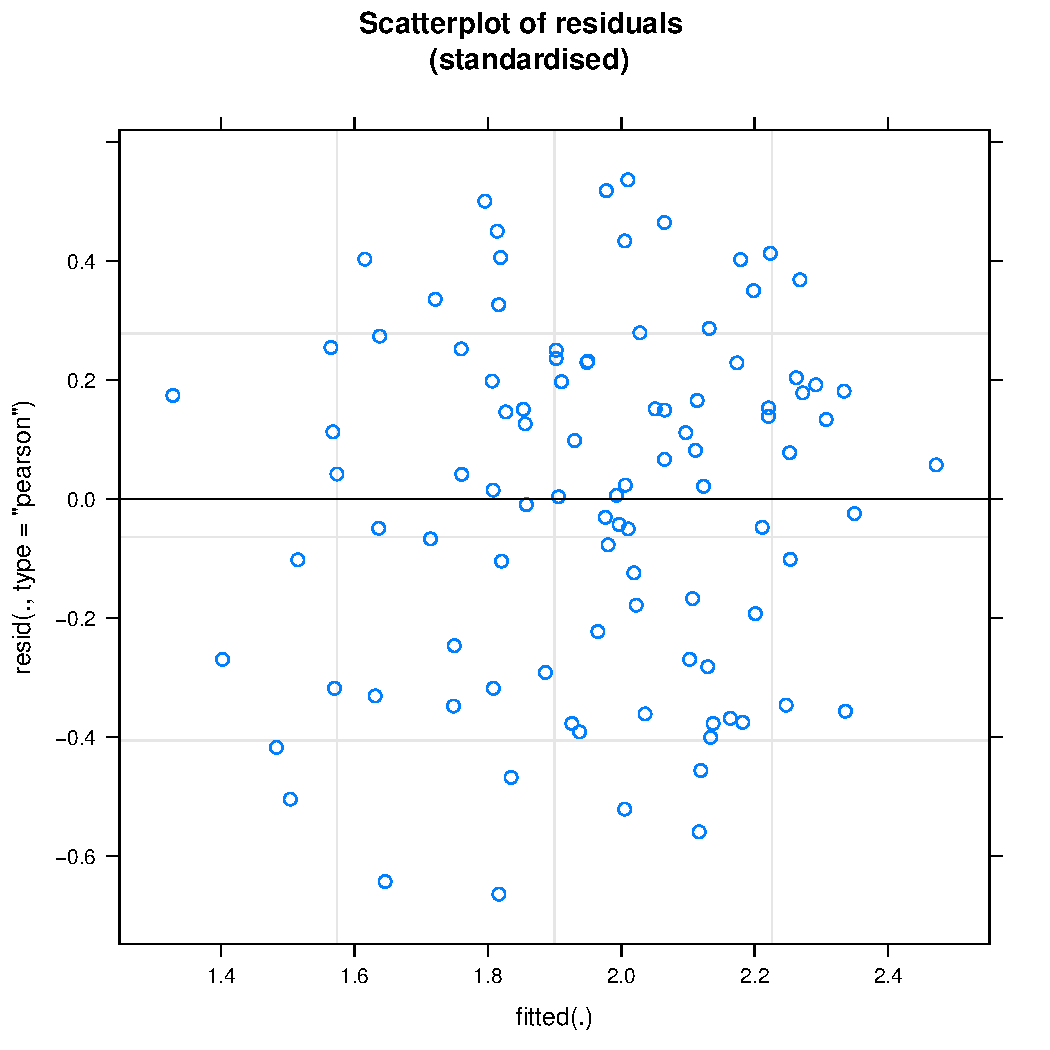
\includegraphics[scale =.4]{images/MLM3aLogScatter.pdf}
  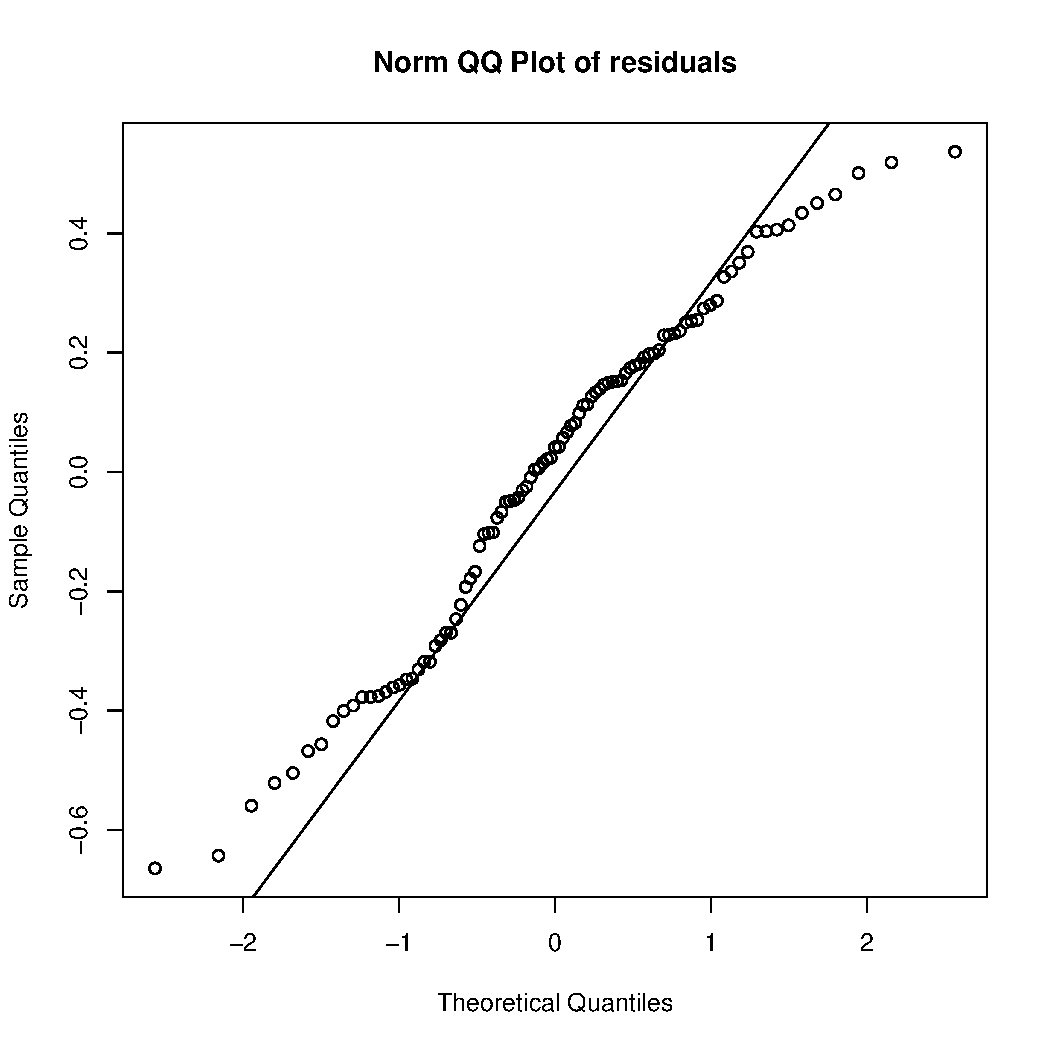
\includegraphics[scale =.4]{images/MLM3aLogQQNorm.pdf}
  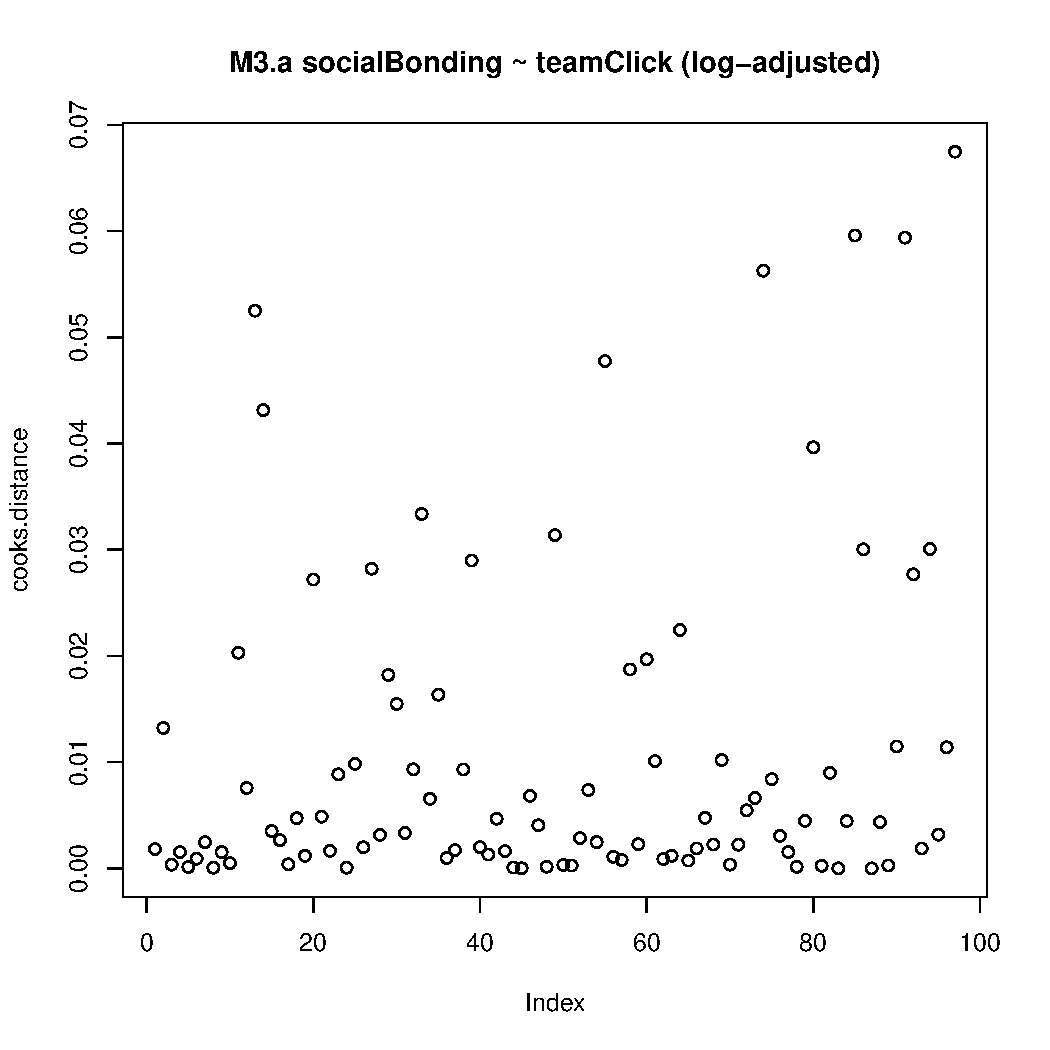
\includegraphics[scale =.4]{images/MLM3aLogCooksD.pdf}
  \caption{Model Assumptions: M3a Joint Action Success predicts Social Bonding (log-transformed)}
  \label{fig:MLM3aLogAssumptions}
\end{figure}








\begin{figure}[htbp]
  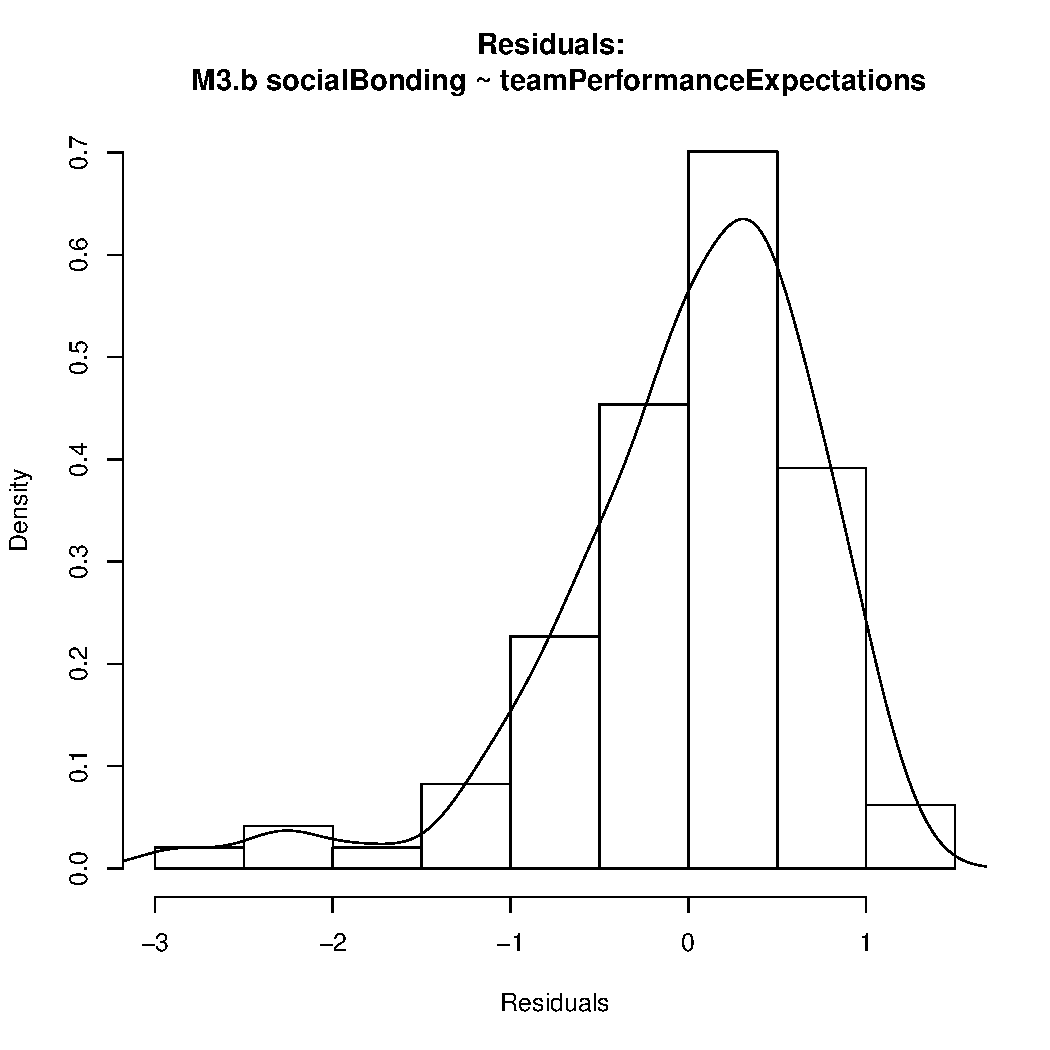
\includegraphics[scale =.4]{images/MLM3bHist.pdf}
  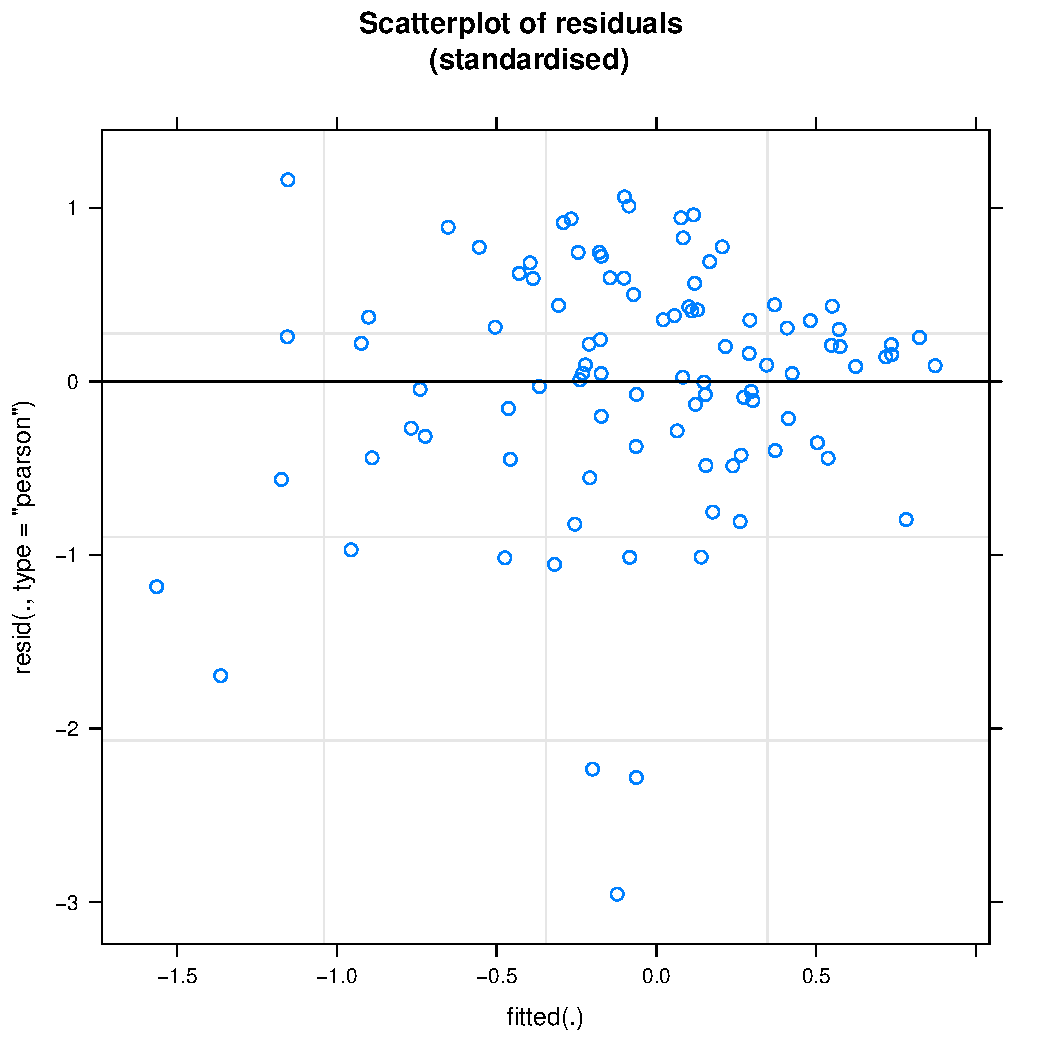
\includegraphics[scale =.4]{images/MLM3bScatter.pdf}
  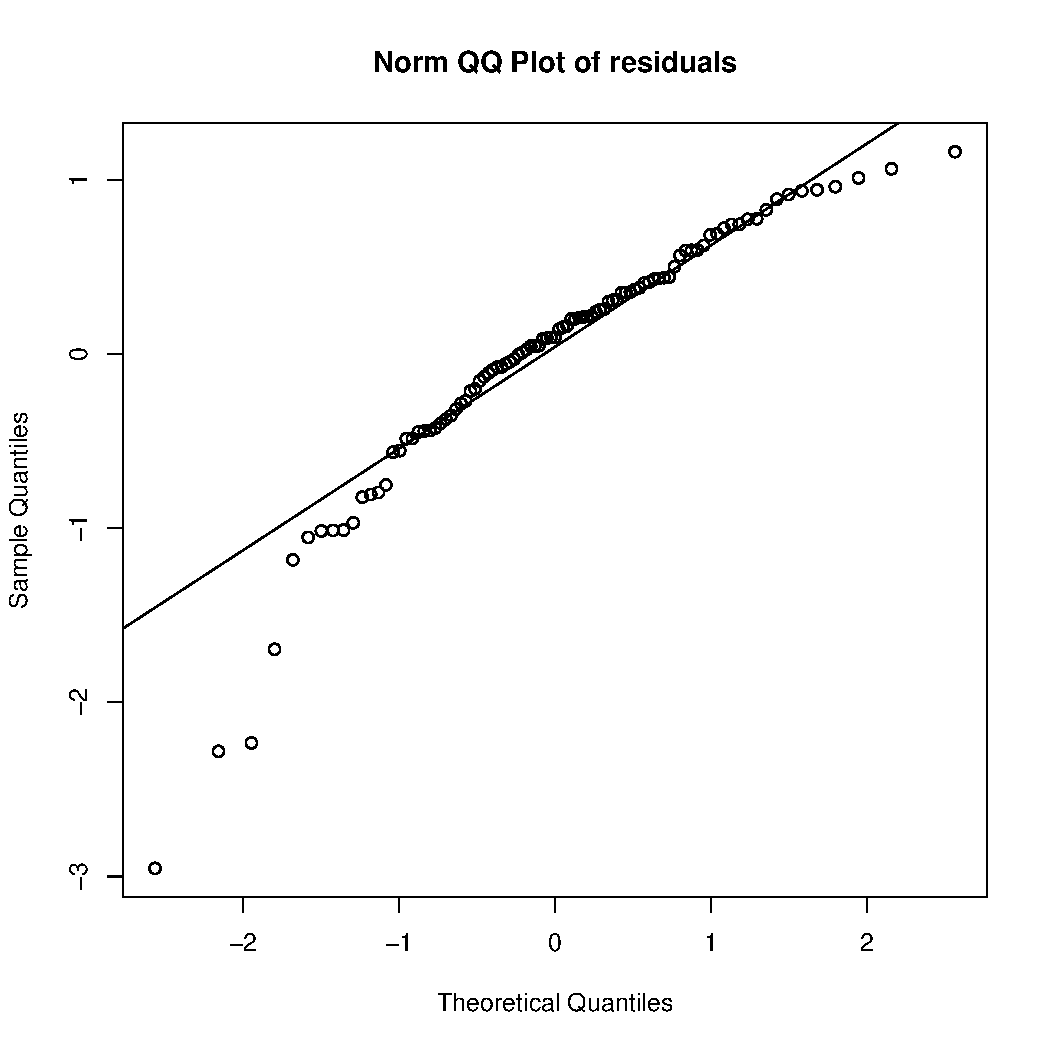
\includegraphics[scale =.4]{images/MLM3bQQNorm.pdf}
  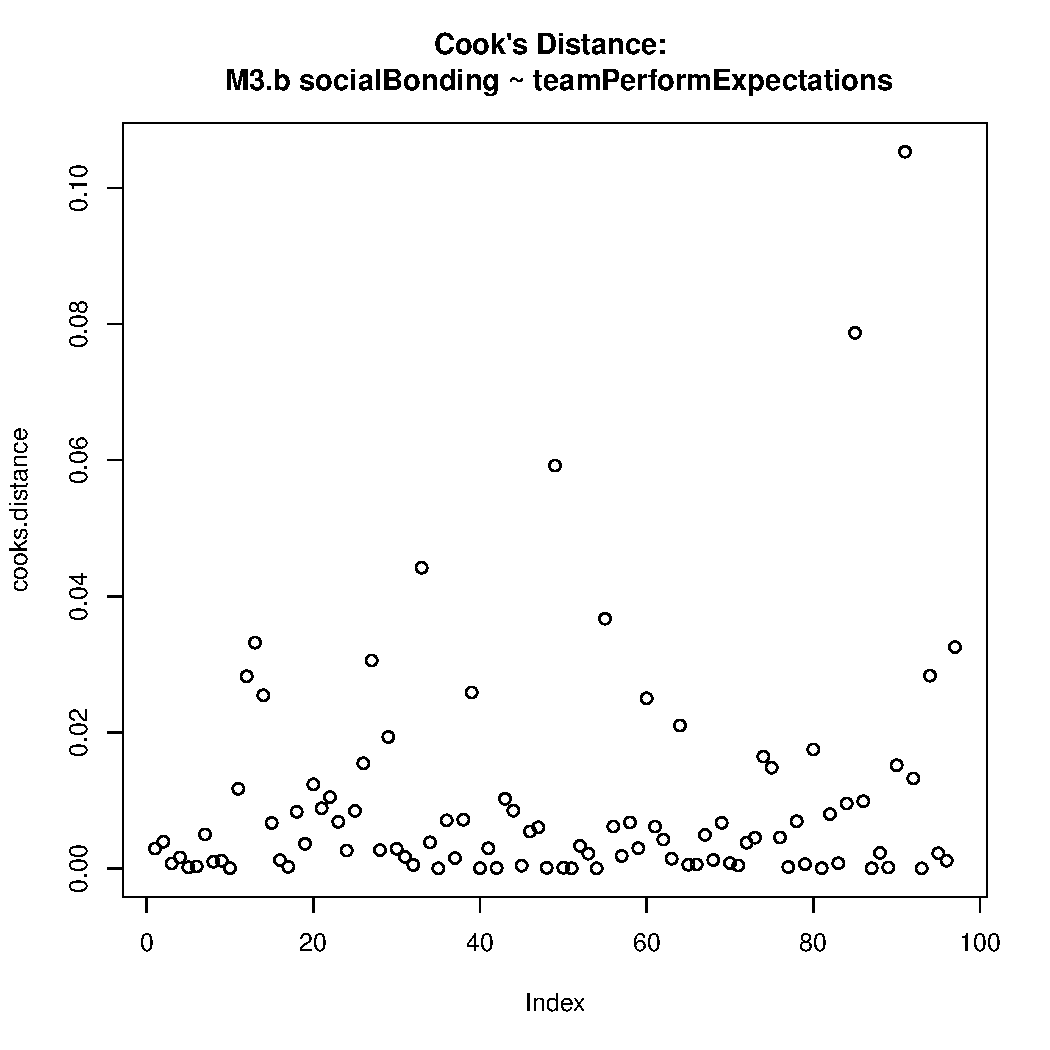
\includegraphics[scale =.4]{images/MLM3bCooksD.pdf}
  \caption{Model Assumptions: M3a Joint Action Success predicts Social Bonding (log-transformed)}
  \label{fig:MLM3bAssumptions}
\end{figure}

\begin{figure}[htbp]
  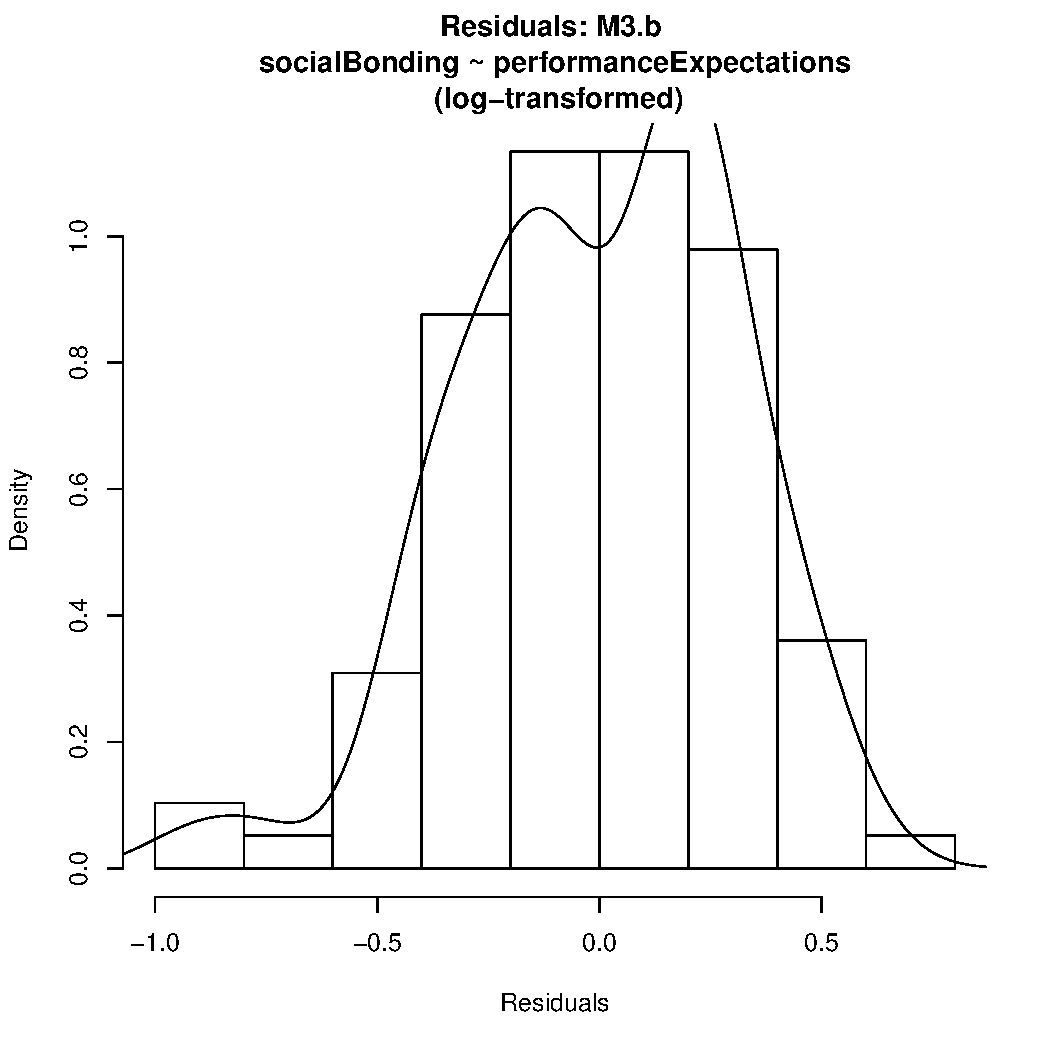
\includegraphics[scale =.4]{images/MLM3bLogHist.pdf}
  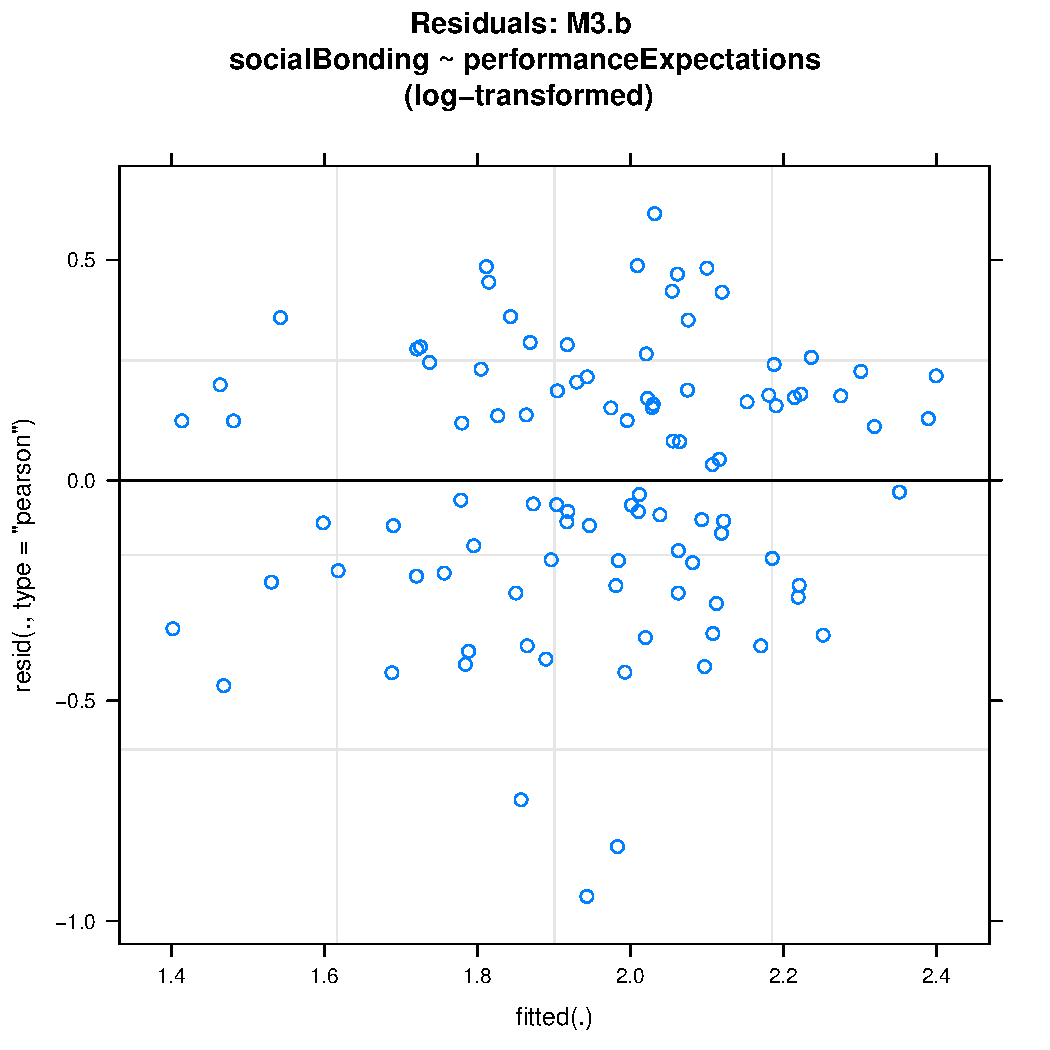
\includegraphics[scale =.4]{images/MLM3bLogScatter.pdf}
  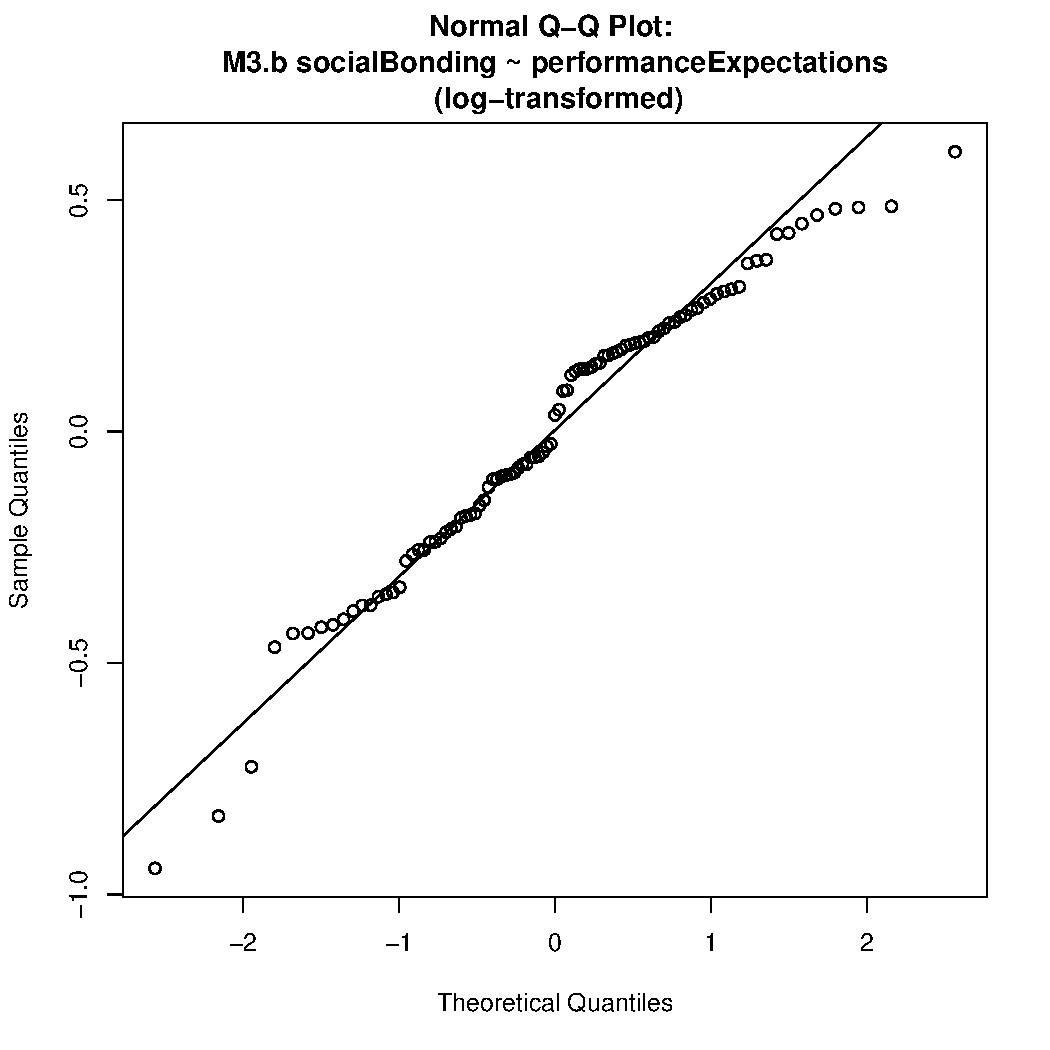
\includegraphics[scale =.4]{images/MLM3bLogQQNorm.pdf}
  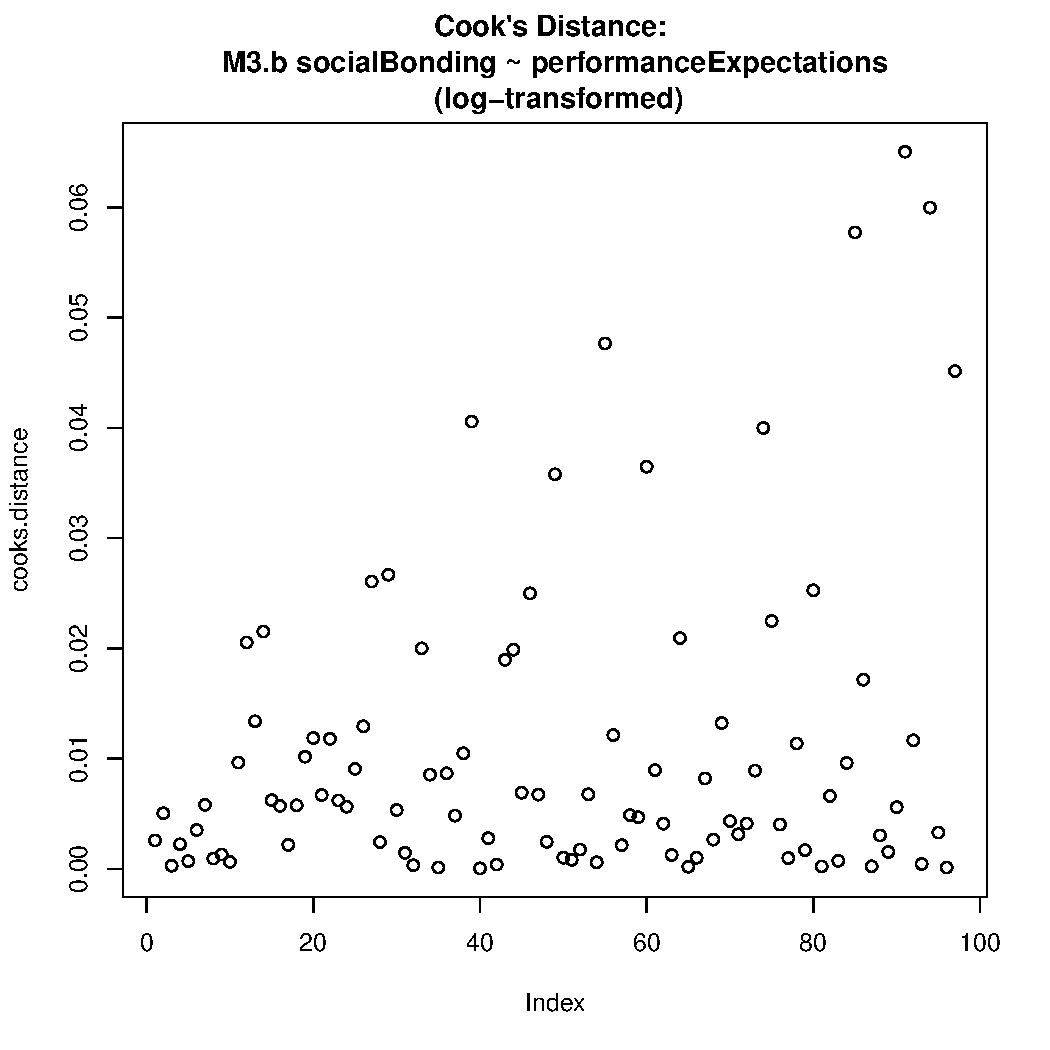
\includegraphics[scale =.4]{images/MLM3bLogCooksD.pdf}
  \caption{Model Assumptions: M3a Joint Action Success predicts Social Bonding (log-transformed)}
  \label{fig:MLM3bLogAssumptions}
\end{figure}






\begin{figure}[htbp]
  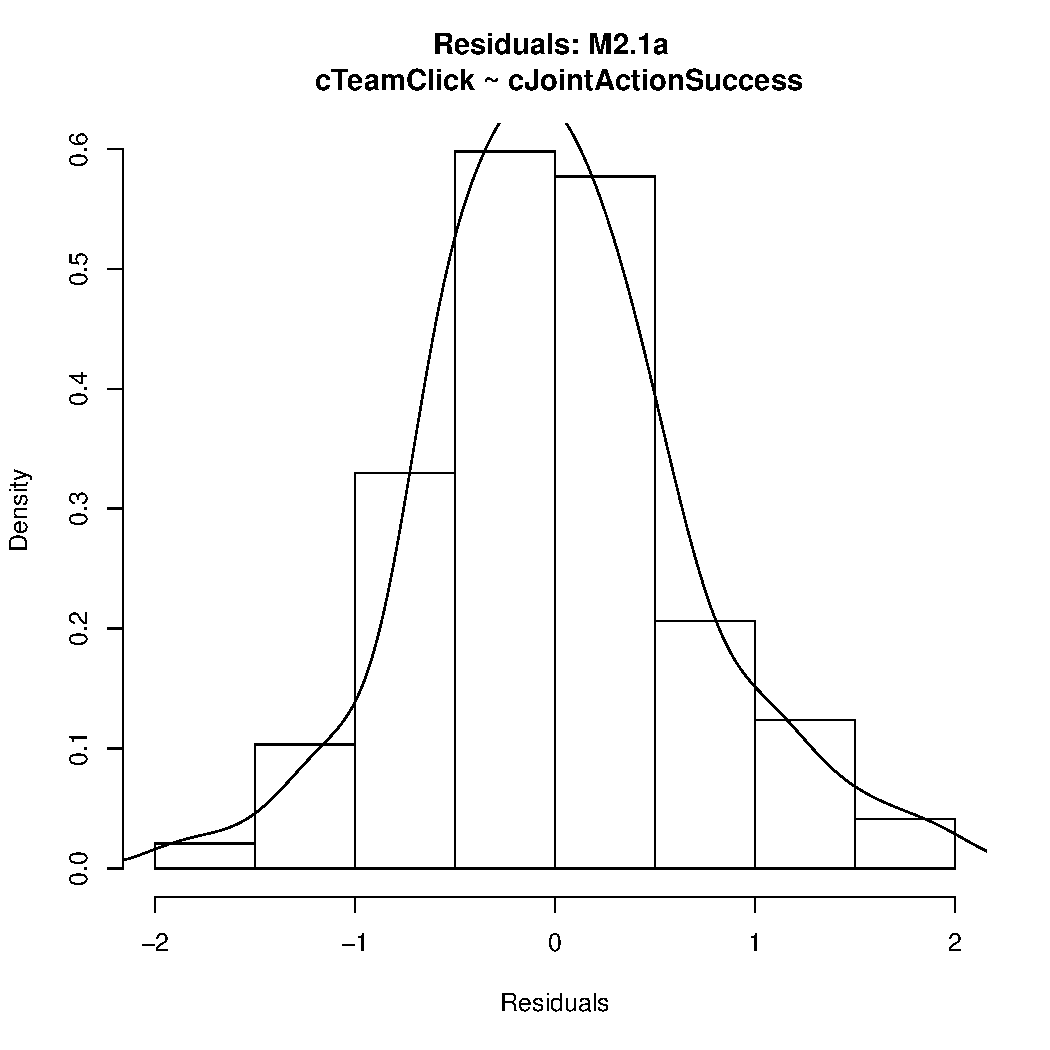
\includegraphics[scale =.4]{images/MLM21aHist.pdf}
  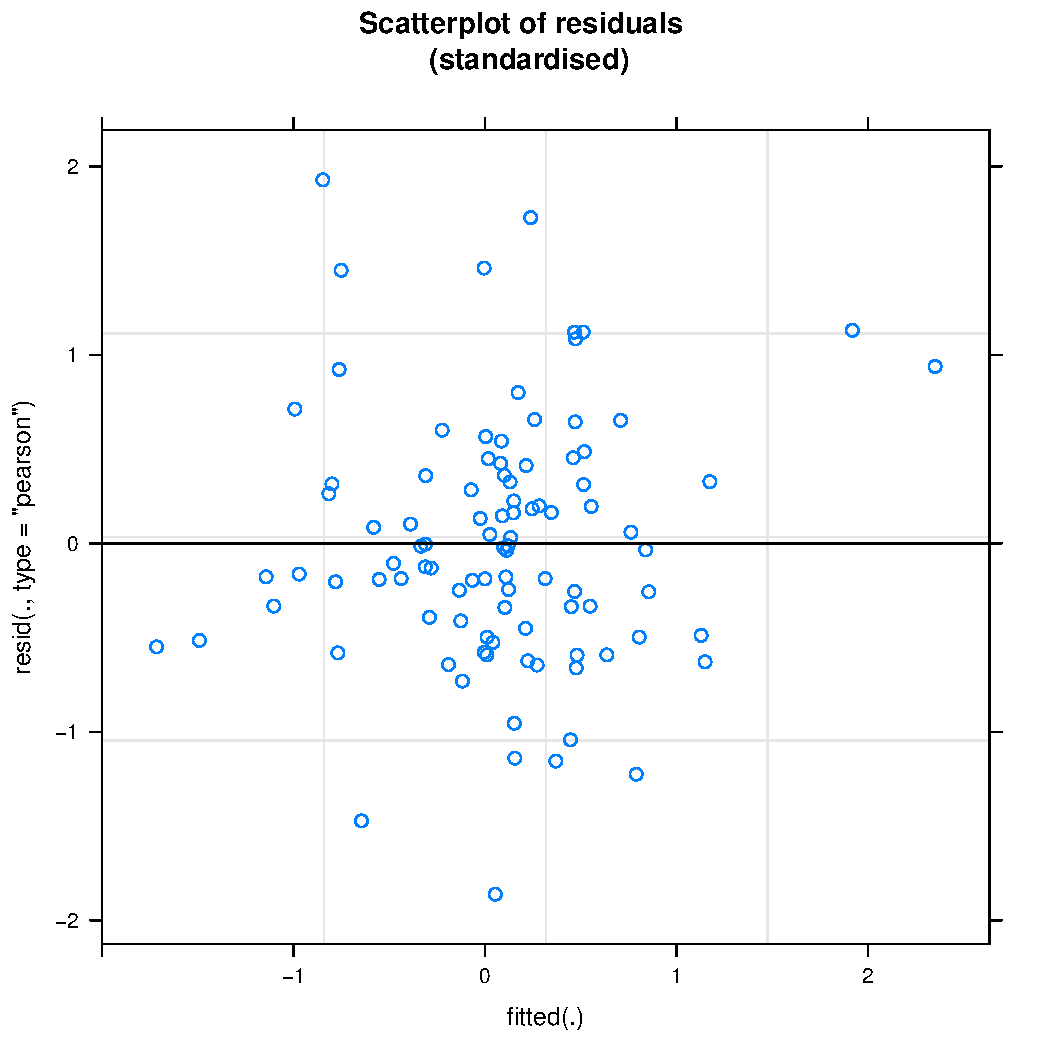
\includegraphics[scale =.4]{images/MLM21aScatter.pdf}
  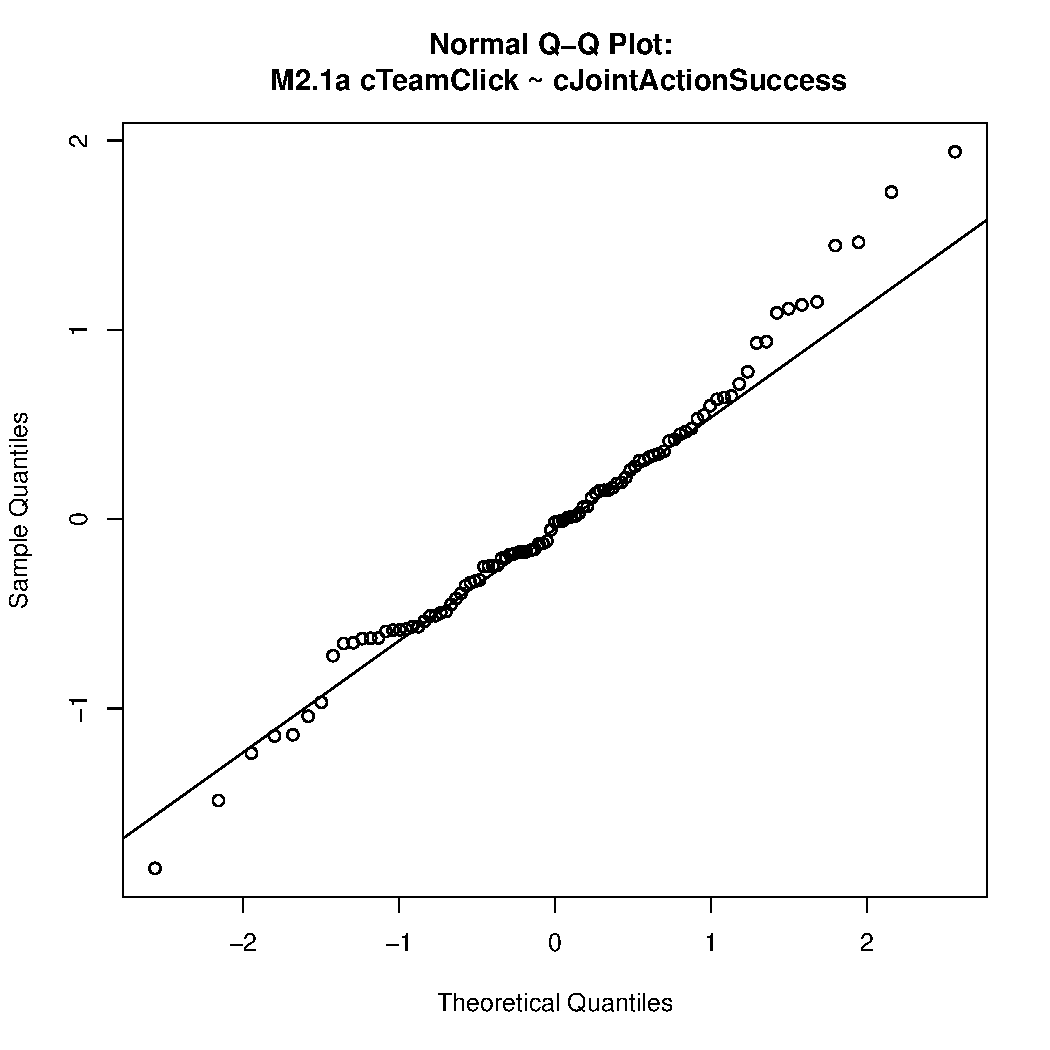
\includegraphics[scale =.4]{images/MLM21aQQNorm.pdf}
  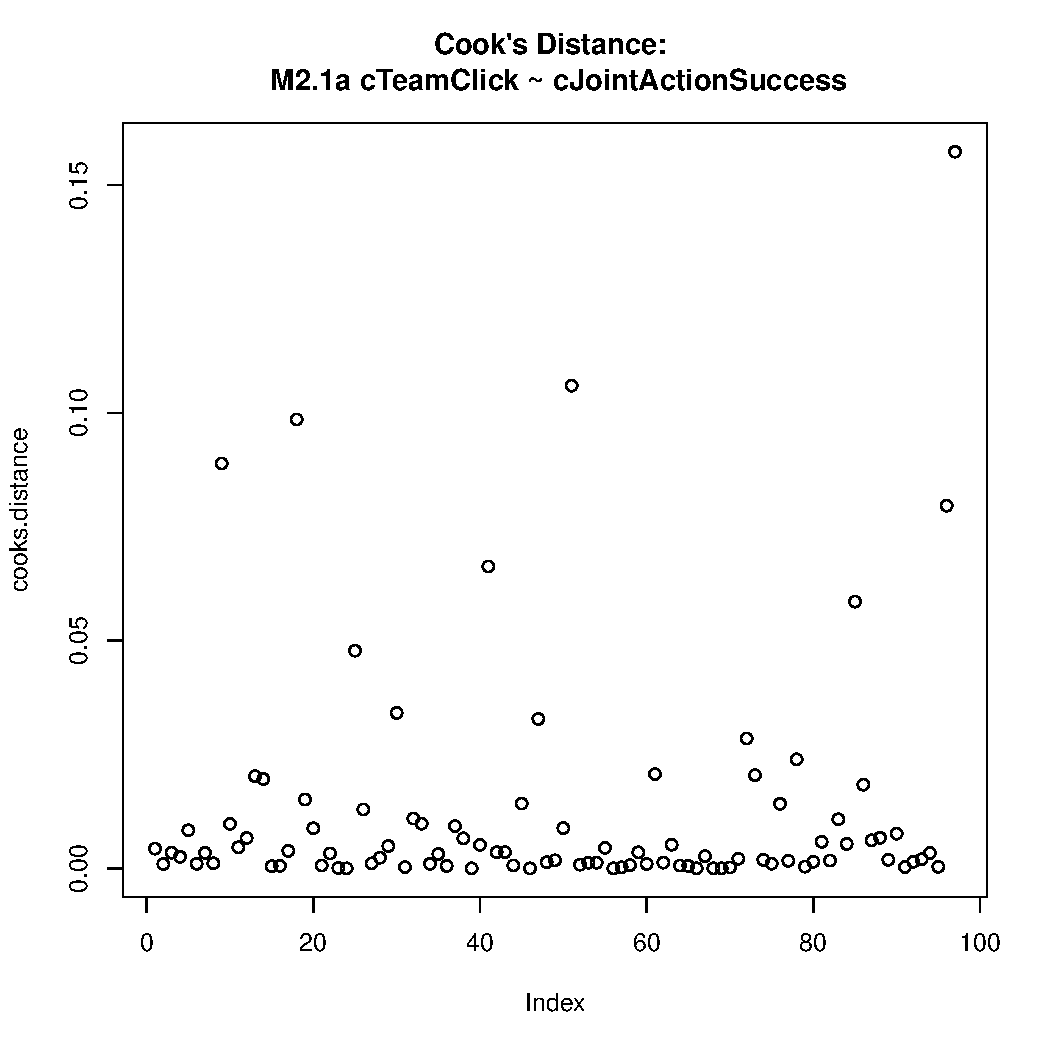
\includegraphics[scale =.4]{images/MLM21aCooksD.pdf}
  \caption{Model Assumptions: M2.1a Change in Joint Action Success predicts change in Team Click}
  \label{fig:MLM21aAssumptions}
\end{figure}





\begin{figure}[htbp]
  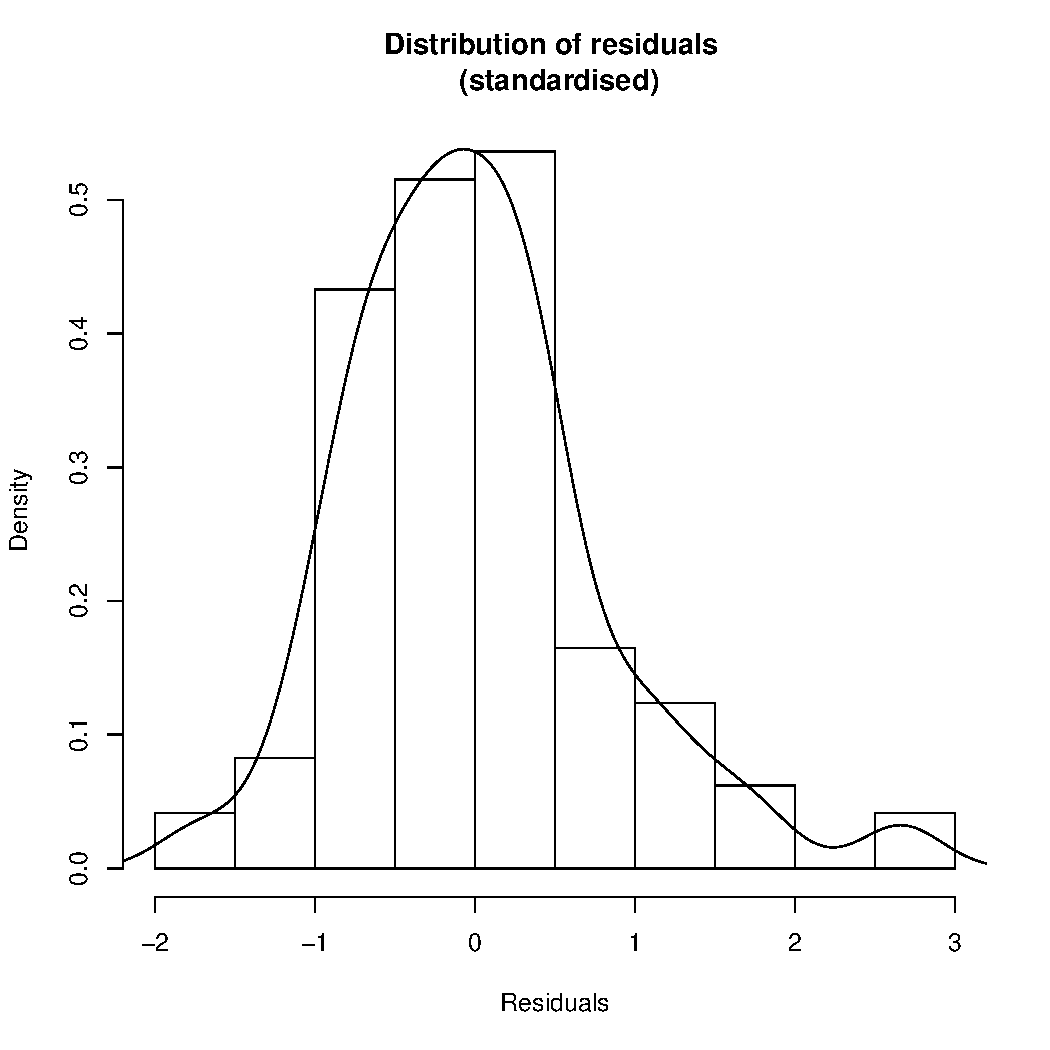
\includegraphics[scale =.4]{images/MLM21bHist.pdf}
  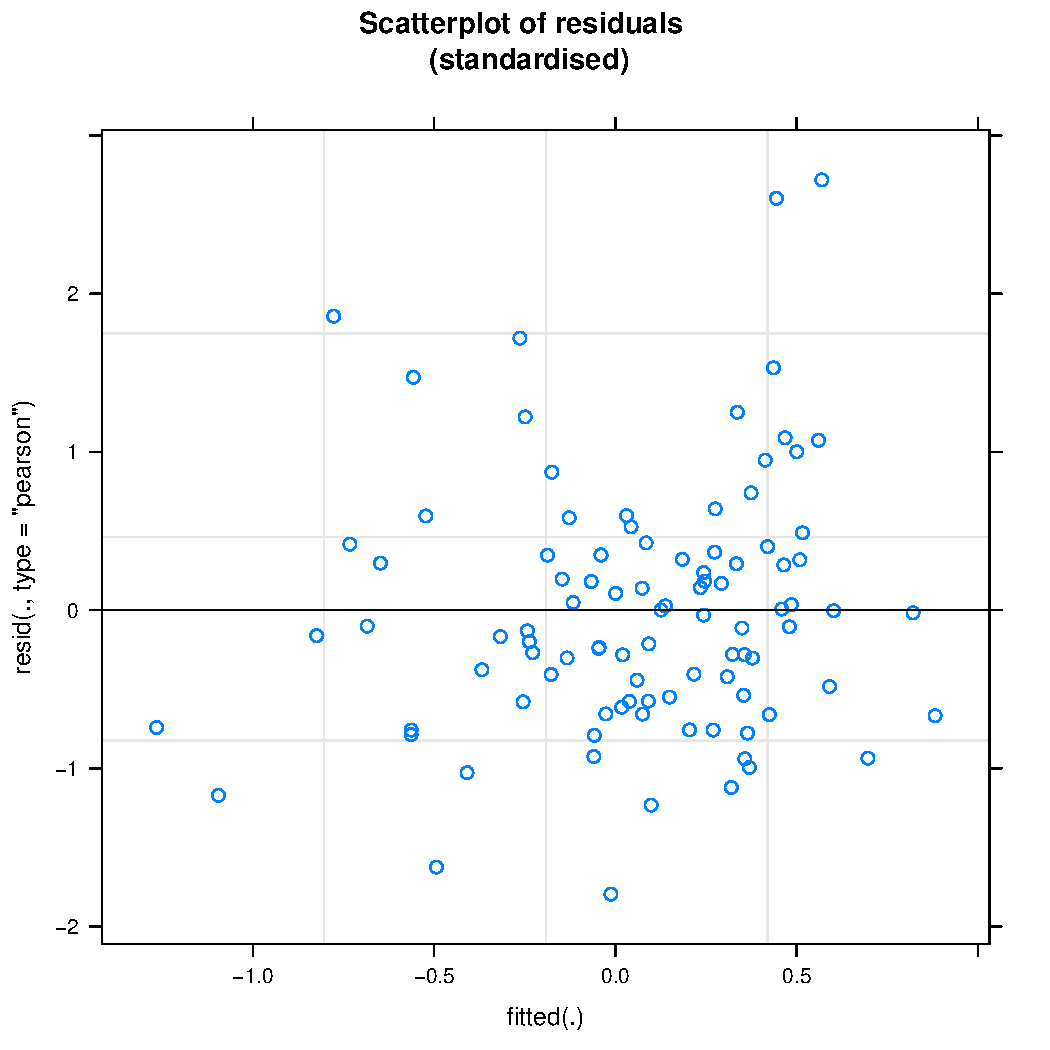
\includegraphics[scale =.4]{images/MLM21bScatter.pdf}
  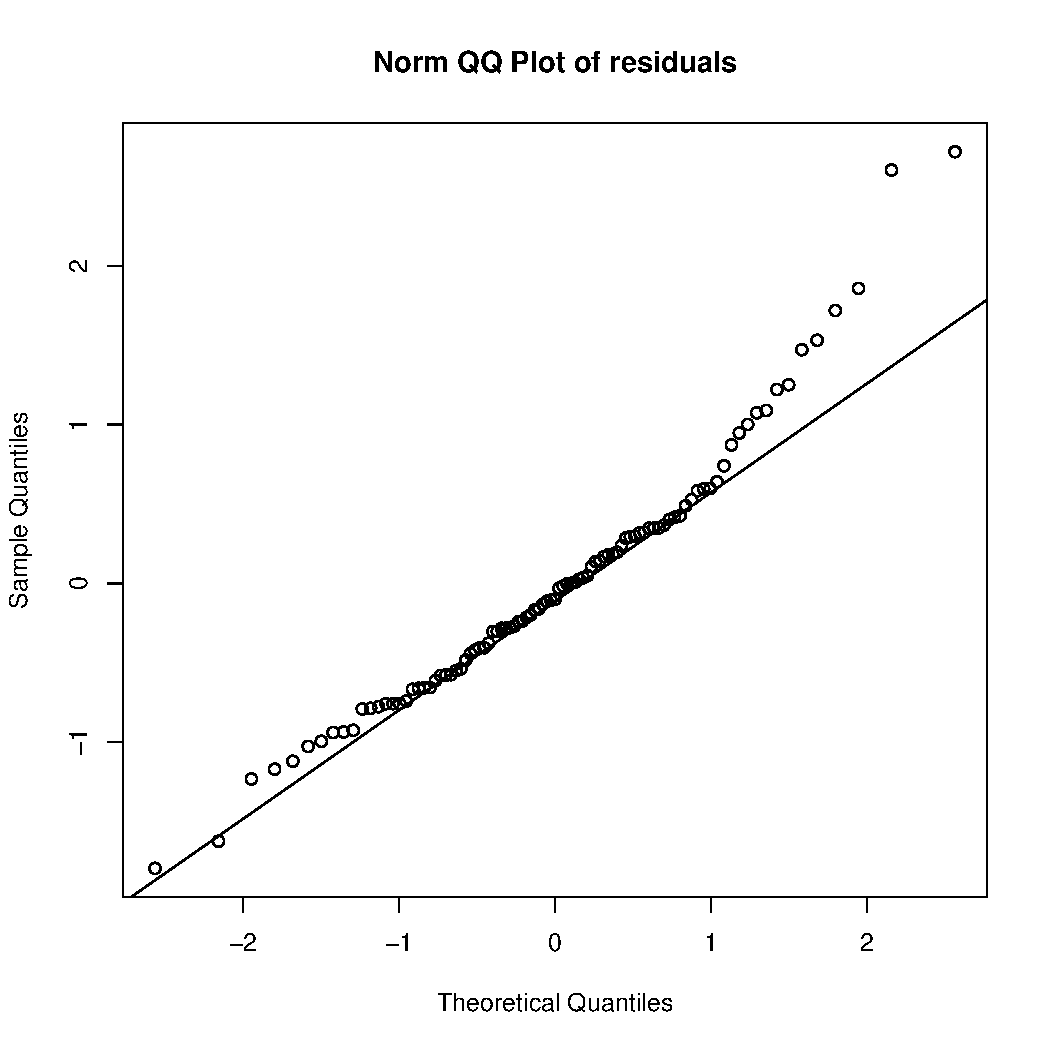
\includegraphics[scale =.4]{images/MLM21bQQNorm.pdf}
  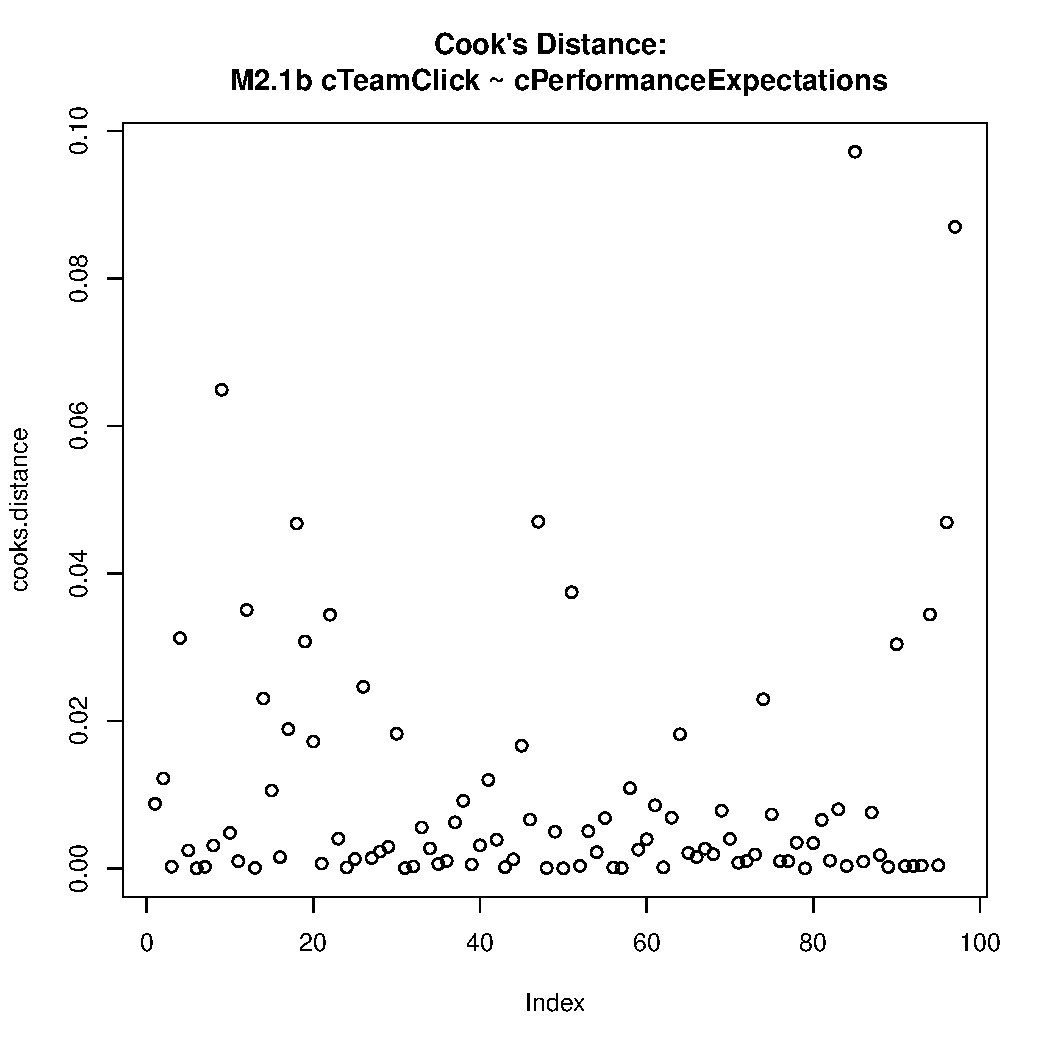
\includegraphics[scale =.4]{images/MLM21bCooksD.pdf}
  \caption{Model Assumptions: M2.1b Team Performance Expectations post-Tournament predicts change in Team Click}
  \label{fig:MLM21bAssumptions}
\end{figure}


\begin{figure}[htbp]
  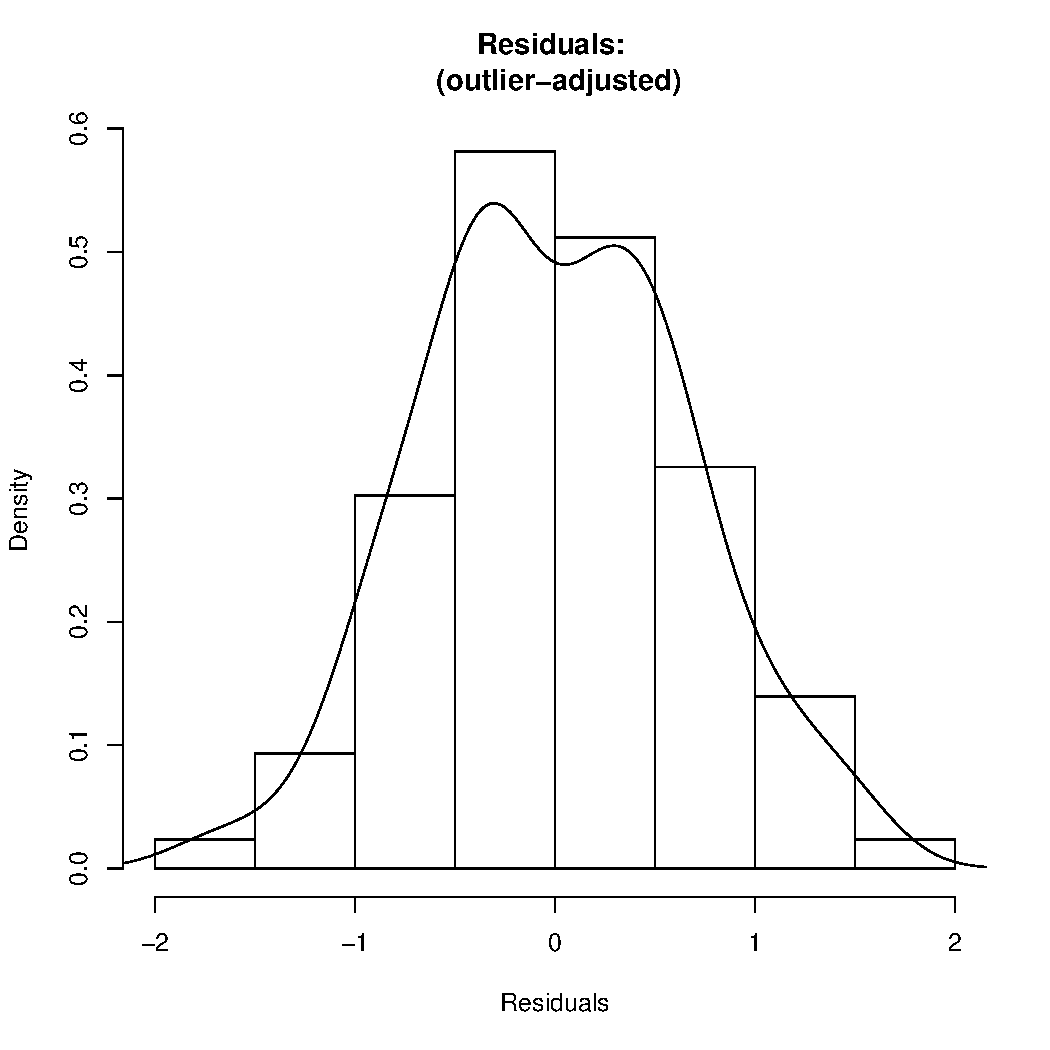
\includegraphics[scale =.4]{images/MLM21bOutHist.pdf}
  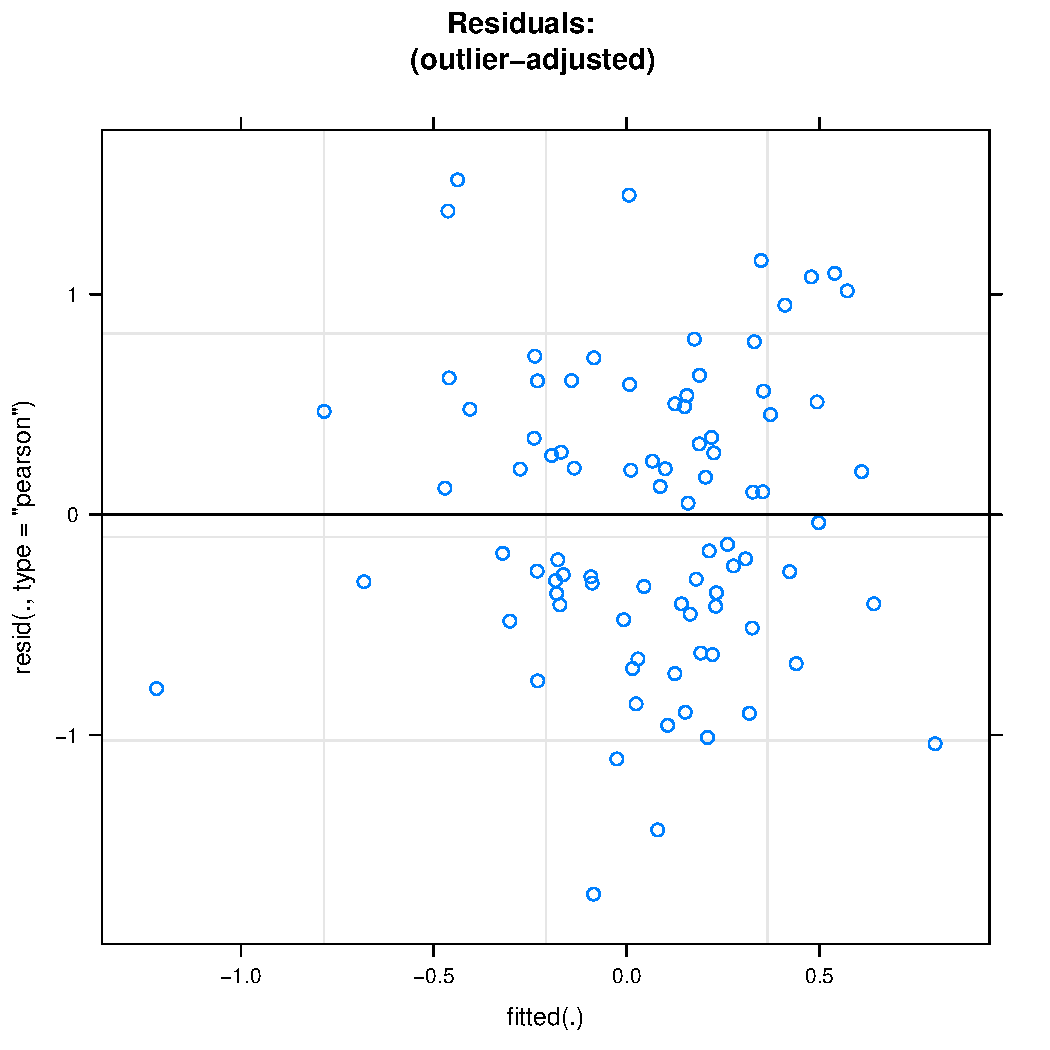
\includegraphics[scale =.4]{images/MLM21bOutScatter.pdf}
  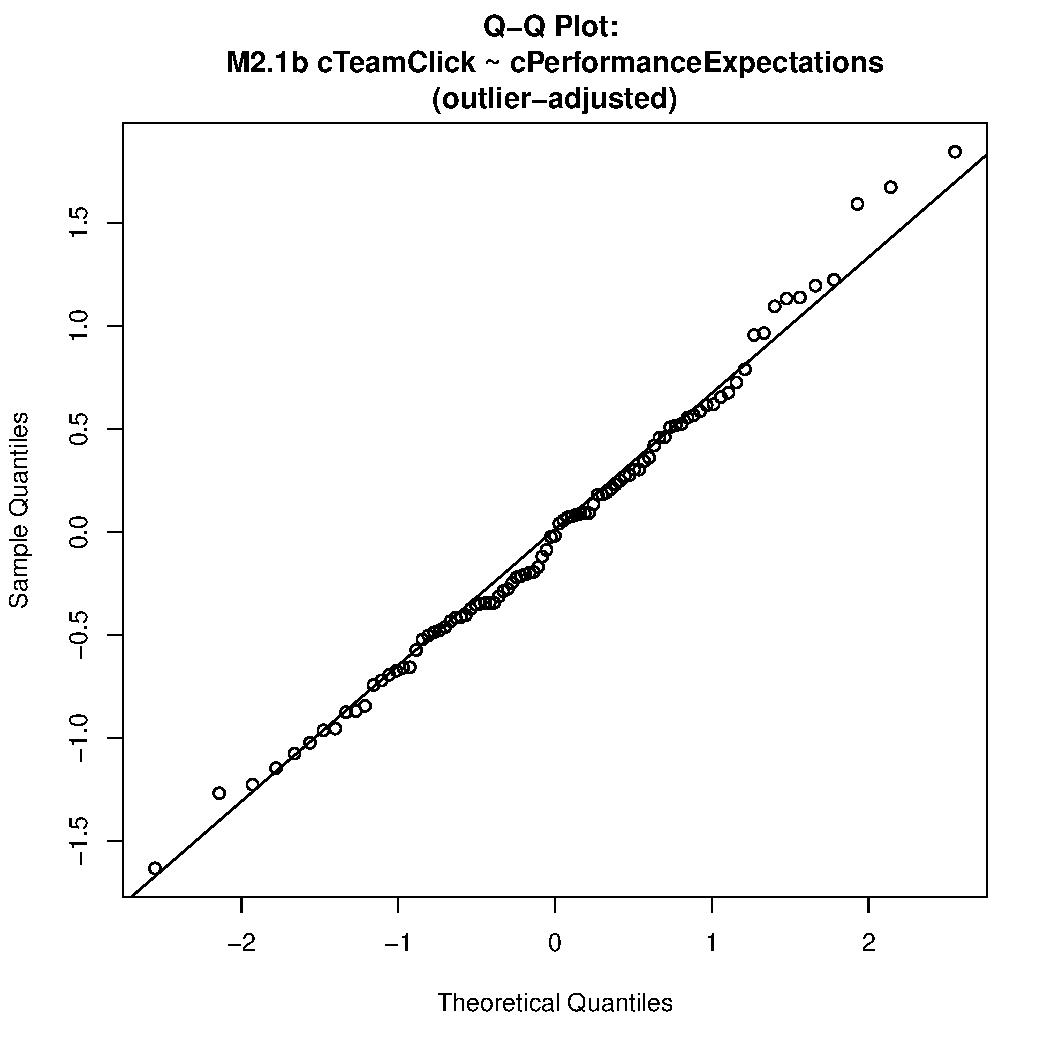
\includegraphics[scale =.4]{images/MLM21bOutQQNorm.pdf}
  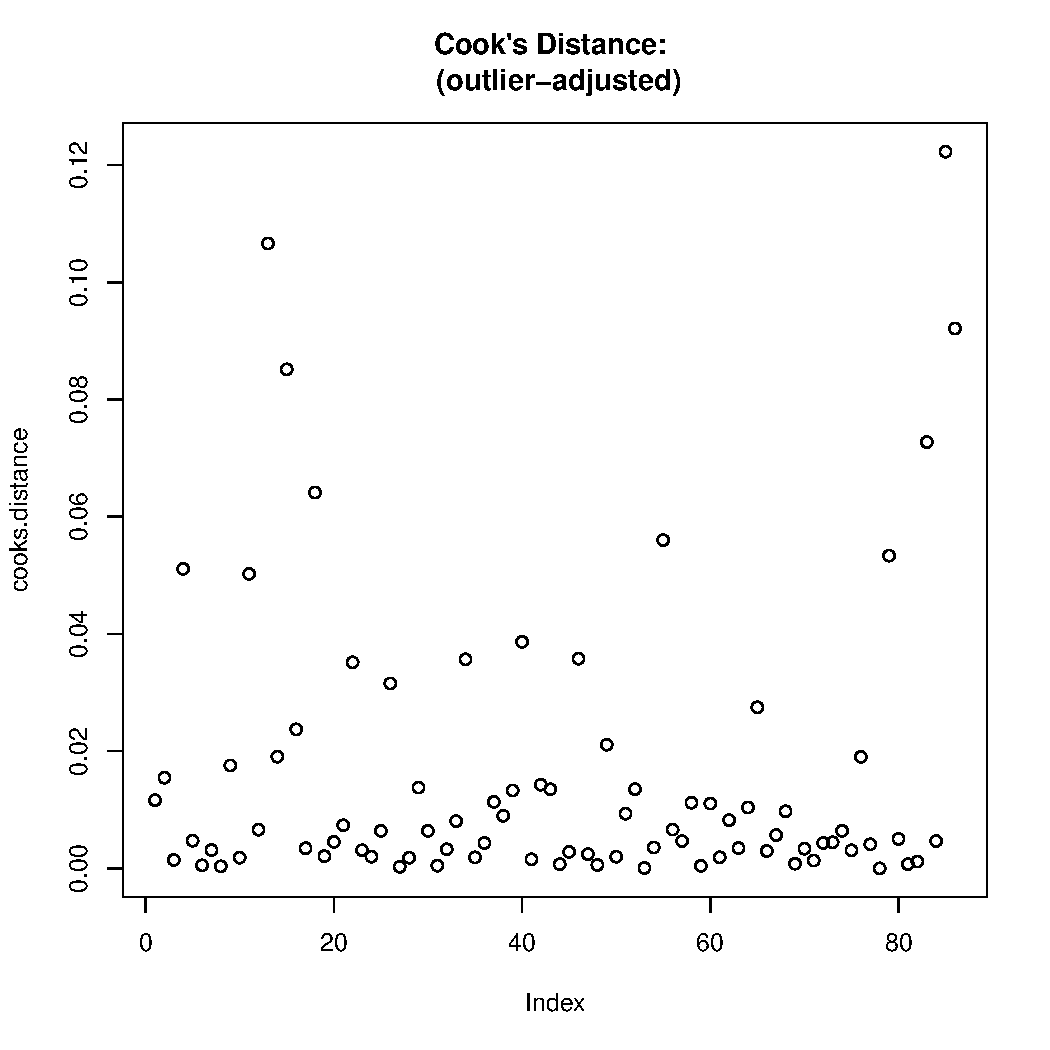
\includegraphics[scale =.4]{images/MLM21bOutCooksD.pdf}
  \caption{Model Assumptions: M2.1b Team Performance Expectations post-Tournament predicts change in Team Click (outliers removed)}
  \label{fig:MLM21bOutAssumptions}
\end{figure}



\begin{figure}[htbp]
  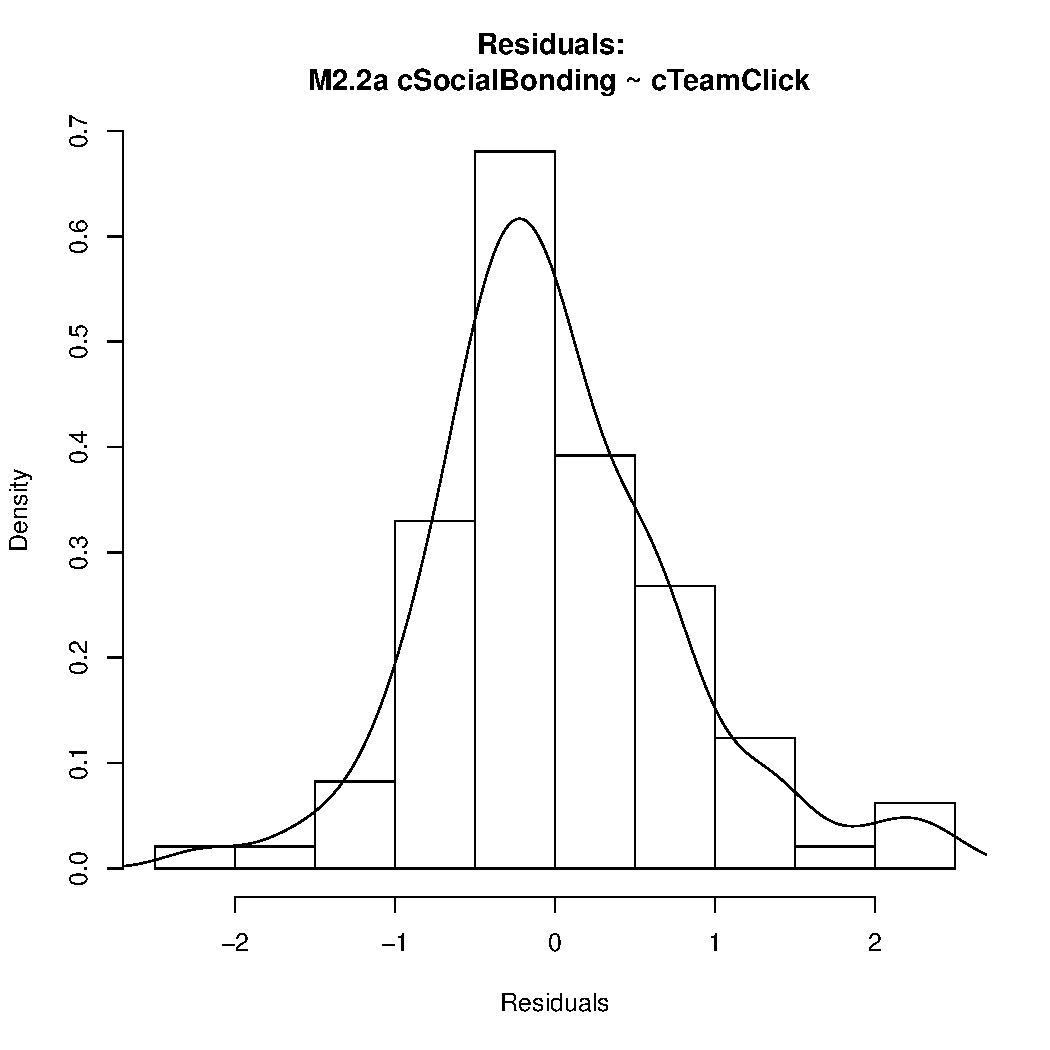
\includegraphics[scale =.4]{images/MLM22aHist.pdf}
  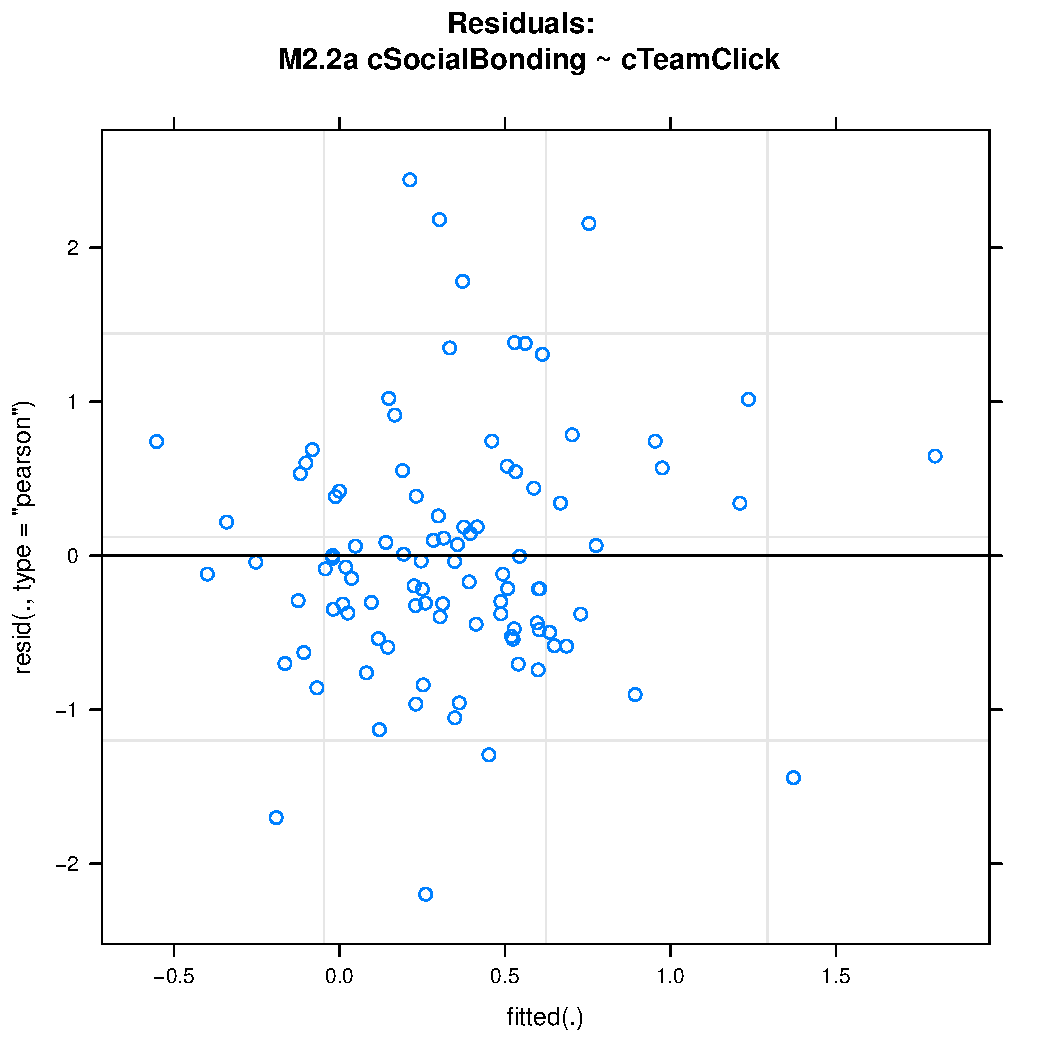
\includegraphics[scale =.4]{images/MLM22aScatter.pdf}
  \includegraphics[scale =.4]{images/MLM22aQQNorm.pdf}
  \includegraphics[scale =.4]{images/MLM22aCooksD.pdf}
  \caption{Model Assumptions: M2.2a Change in Team Click predicts change in Social Bonding}
  \label{fig:MLM22aAssumptions}
\end{figure}


\begin{figure}[htbp]
  \includegraphics[scale =.4]{images/MLM23aHist.pdf}
  \includegraphics[scale =.4]{images/MLM23aScatter.pdf}
  \includegraphics[scale =.4]{images/MLM23aQQNorm.pdf}
  \includegraphics[scale =.4]{images/MLM23aCooksD.pdf}
  \caption{Model Assumptions: M2.3a Change in Joint Action Success predicts change in Social Bonding}
  \label{fig:MLM23aAssumptions}
\end{figure}



\begin{figure}[htbp]
  \includegraphics[scale =.4]{images/MLM23aHist.pdf}
  \includegraphics[scale =.4]{images/MLM23aScatter.pdf}
  \includegraphics[scale =.4]{images/MLM23aQQNorm.pdf}
  \includegraphics[scale =.4]{images/MLM23aCooksD.pdf}
  \caption{Model Assumptions: M2.3a Change in Joint Action Success predicts change in Social Bonding}
  \label{fig:MLM23aAssumptions}
\end{figure}






\subsubsection{Additional Analysis: What predicts change in fusion to family?}
Both verbal and pictorial measures of fusion to team did not vary significantly in pre-post Tournament measures (see descriptives Table ~\ref{tab:factorsPrePostSummary}).  Interestingly, the pictorial measure of fusion to family did increase significantly between pre- and post-Tournament measurements.  Exploratory analysis was performed to investigate the possible correlates of this increase. In line with the predictions of this study, we tested whether 1) changes in perceptions of Joint Action Success, 2) Team Click, and 3) their interaction (Joint Action Success x Team Click) predicted change in fusion to family.

\myparagraph{$\Delta$Fusion Family $\sim$ $\Delta$Joint Action Success}
The first model revealed a significant effect of change in perceptions of joint-action success and change in fusion to family, $\beta = .43$ ($95\% CI =  .07, .79$), $SE = .18$, $t(6.96) = 2.34$, $p = .$, $marginal R^2 = .11$, $conditional R^2 = .14$.  The distribution of residuals indicated a poor model fit, ($W = 0.90$, $p < .00001$), due to high kurtosis ($> 2$), but not skew (.30). Given that log-transformation was not appropriate for normalising kurtosis \citep{Glass1972}, the analysis was re-run after excluding influential outliers.  The adjusted model was a much better fit, with model residuals normally distributed around zero, ($W = 0.99$, $p-value < .60$), see Table ~\ref{tab:MLM25acFusioncJointAction}. The model confirmed a significant positive relationship between change in perceptions of joint-action success and change in fusion to family, $\beta = .36$ ($95\% CI =  .19, .52$), $SE = .08$, $t() = 4.36$, $p = .$, $marginal R^2 = .32$, $conditional R^2 = .32$.


% Table created by stargazer v.5.2 by Marek Hlavac, Harvard University. E-mail: hlavac at fas.harvard.edu
% Date and time: Tue, Jun 27, 2017 - 10:42:15
\begin{table}[!htbp] \centering 
  \caption{cFusionFamily ~ jointActionSuccess} 
  \label{tab:MLM25acFusioncJointAction} 
\footnotesize 
\begin{tabular}{@{\extracolsep{5pt}}lcc} 
\\[-1.8ex]\hline 
\hline \\[-1.8ex] 
 & \multicolumn{2}{c}{\textit{Dependent variable:}} \\ 
\cline{2-3} 
\\[-1.8ex] & cFusionFamily & fusionPictorialFamilyChangeOut \\ 
 &  & outliers removed \\ 
\\[-1.8ex] & (1) & (2)\\ 
\hline \\[-1.8ex] 
 (constant) & 0.12 & $-$0.04 \\ 
  & (0.66) & (0.32) \\ 
  & & \\ 
 cJointActionSuccess & 0.43$^{**}$ & 0.50$^{***}$ \\ 
  & (0.18) & (0.10) \\ 
  & & \\ 
 cIndPerformanceSuccess & $-$0.46$^{**}$ & $-$0.01 \\ 
  & (0.20) & (0.10) \\ 
  & & \\ 
 teamPerformanceExpectations & $-$0.01 & 0.002 \\ 
  & (0.01) & (0.004) \\ 
  & & \\ 
 indPerformanceExpectations & 0.001 & $-$0.003 \\ 
  & (0.01) & (0.004) \\ 
  & & \\ 
 objectiveCompetence & 0.27 & 0.06 \\ 
  & (0.19) & (0.09) \\ 
  & & \\ 
 subjectiveCompetence & 0.06 & $-$0.0003 \\ 
  & (0.16) & (0.08) \\ 
  & & \\ 
 finalRank & 0.10 & $-$0.02 \\ 
  & (0.08) & (0.04) \\ 
  & & \\ 
 minutesTotal & $-$0.002 & 0.01 \\ 
  & (0.01) & (0.004) \\ 
  & & \\ 
\hline \\[-1.8ex] 
Marginal R-squared & .11 & .32 \\ 
Conditional R-squared & .14 & .32 \\ 
Observations & 97 & 97 \\ 
Log Likelihood & $-$173.00 & $-$104.99 \\ 
Akaike Inf. Crit. & 372.00 & 235.98 \\ 
Bayesian Inf. Crit. & 405.48 & 269.45 \\ 
\hline 
\hline \\[-1.8ex] 
\textit{Note:}  & \multicolumn{2}{r}{$^{*}$p$<$0.1; $^{**}$p$<$0.05; $^{***}$p$<$0.01} \\ 
\end{tabular} 
\end{table} 

% Table created by stargazer v.5.2 by Marek Hlavac, Harvard University. E-mail: hlavac at fas.harvard.edu
% Date and time: Tue, Jun 27, 2017 - 10:42:15
\begin{table}[!htbp] \centering 
  \caption{cFusionFamily ~ jointActionSuccess} 
  \label{tab:MLM25acFusioncJointAction} 
\footnotesize 
\begin{tabular}{@{\extracolsep{5pt}} ccc} 
\\[-1.8ex]\hline 
\hline \\[-1.8ex] 
$0.05$ & $0.01$ & $0.001$ \\ 
\hline \\[-1.8ex] 
\end{tabular} 
\end{table} 


%Need to do a multivariate regression here with family, country, team as outcomes?
\myparagraph{$\Delta$fusionFamily $\sim$ $\Delta$Team Click}

This model revealed that change in feelings of team-click was not a significant predictor of change in fusion to family, $\beta = .07$ ($95\% CI =  -.30, .44$), $SE = .19$, $t() = .38$, $p = .$, $marginal R^2 = .04$, $conditional R^2 = .07$. No other predictors in the model were statistically significant.

\myparagraph{$\Delta$fusionFamily $\sim$  $\Delta$Joint Action Success $\times$ $\Delta$Team Click}

The final model included an interaction between change in perceptions of joint-action success and change in feelings of team click as possible predictor of change in fusion to family.  Results of the model revealed that the interaction between change in perceptions of joint-action success and change in feelings of team-click was a significant positive predictor of change in fusion to family, $\beta = .22$ ($95\% CI =  .02, .41$), $SE = .10$, $t() = 2.22$, $p = .$, $marginal R^2 = .17$, $conditional R^2 = .23$. Model residuals were non-normally distributed, ($W = 0.93$, $p < .00001$).\\

This result is consistent with ethnographic findings, whereby the family unit is elevated above the team and other priorities.  This results will be considered in more depth once ethnographic analysis has also been completed.














\subsection{Analysis of post-Tournament data}
%\subsubsection{Roadmap of post-Tournament Analysis}
Analysis of the post-Tournament data proceeded by testing predictions associated with the overarching hypothesis, that higher perceptions of joint-action success would lead to higher levels of social bonding, mediated by feelings of ``team click''.

The first step was to assess whether the two variables hypothesised to be relevant to perceived joint-action success, 1) perceptions of team performance (Joint Action Success) and 2) perceptions of team performance relative to prior expectations (Team Performance Expectations), predicted feelings of team click (Team Click). Controlling for athlete perceptions of individual performance success, subjective and objective technical competence, Tournament performance measures, and variation attributable to team membership (random effect), linear mixed-effect regression models were used to test the following predictions:

\begin{description}
  \item [Prediction 1.a] Joint Action Success  $\rightarrow$ Team Click
  \item [Prediction 1.b] Team Performance Expectations $\rightarrow$ Team Click
  \item [Prediction 1.c] Joint Action Success $\rightarrow$ Team Click, moderated by Team Performance Expectations
\end{description}

Next, the relationship between team click (Team Click) and social bonding (Social Bonding) was tested, controlling for subjective and objective technical competence, Tournament performance measures, and variation attributable to team membership (random effect):

\begin{description}
  \item [Prediction 2.a] Team Click $\rightarrow$ Social Bonding
\end{description}

Following this, the direct relationships between two predictor variables of interest (Joint Action Success and Team Performance Expectations) and social bonding was tested:

\begin{description}
  \item [Prediction 3.a] Joint Action Success $\rightarrow$ Social Bonding
  \item [Prediction 3.b] Team Performance Expectations $\rightarrow$ Social Bonding
\end{description}

Finally, a mediation analysis was performed to formally test whether feelings of team click mediated a direct relationship between perceptions of joint-action success and social bonding.

\begin{description}
\item[Prediction 4.a Mediation Analysis] Joint Action Success $\rightarrow$ Team Click $\rightarrow$ Social Bonding
\item[Prediction 4.b Mediation Analysis] Team Performance Expectations $\rightarrow$ Team Click $\rightarrow$ Social Bonding
\end{description}


















\subsection{Post-Tournament Results}

\subsubsection{1.a: Joint Action Success predicts Team Click}
\subsubsection{1.b Team Performance Expectations predict Team Click}
\subsubsection{1.c Team Performance Expectations moderates the effect of Joint Action Success on team Click}

%Findings from the first collection of models generally supported predictions. Team performance factors\nobreakdashperceptions of team component performance success and team performance relative to prior expectations\nobreakdashbut not individual performance factors significantly predicted team click, when controlling for subjective and objective competence, and Tournament performance measures.  The interaction effect of joint-action success and team performance expectations violation on team click was not significant.  Additionally, the low coefficient value for the model in which teamPerformanceExpectations predicted team click was low, indicating that this result should be treated with some caution.  Taken together, however, these results provide evidence for the predictions that perceptions of joint-action success is linked to feelings of team click.  Team performance expectations do not interact with perceptions of joint action to enhance feelings of team click, but rather function independently to predict team click, with those athletes who were experienced more positive violations of expectations also reporting higher levels of team click.

\subsubsection{2.a Team Click predicts Social Bonding}
\subsubsection{3.a Joint Action Success predicts Social Bonding}
\subsubsection{3.b Team Performance Expectations predicts Social Bonding} % very small effect
\subsubsection{4.a Mediation analysis: Joint Action Success predicts Social Bonding, mediated by Team Click}
\subsubsection{4.b Mediation analysis: Team Performance Expectations predicts Social Bonding, mediated by Team Click}

%\begin{figure}[htbp]
%  \includegraphics{finalDocuments/images/MLM4aResiduals.pdf}
%  \includegraphics{finalDocuments/images/MLM4aQQNorm.pdf}
%  \includegraphics{finalDocuments/images/MLM4aResiduals.pdf}
%  \includegraphics{finalDocuments/images/MLM4aCooksD.pdf}
%  \caption{M4a Mediation Analysis}
%  \label{fig:MLM4aAssumptions}
%\end{figure}

% (Baer et al 2006: 147) One method for constructing CIs assumes normality for the sampling distributions of the estimates. Under this assumption, 95% CIs for the average indirect effect and average total effect are obtained as Alternatively, one could perform a null hypothesis test by forming the critical ratio of each estimate to its standard error and comparing the result with the critical value of the z distribution. In andthe as- sumption of normality for the sampling distributions will not hold exactly, given that aˆb ˆ is a product of normally distributed estimates (and hence will not be normal). The deviation from normality may be small enough, however, that the CIs or significance tests will still be reasonably accurate.

%An alternative method for constructing CIs that may hold promise is the Monte Carlo (MC) method of MacKinnon et al. (2004). In this approach, the sampling distribution for the effect of interest is not assumed to be normal and is instead simulated from the model estimates and their asymptotic variances and covariances (a form of parametric bootstrap- ping). For instance, to simulate the sampling distribution of the average indirect effect, one would define a multinormal distribution with means equal to a ˆ, b ˆ, and ˆ aj ,bj and covariance matrix equal to the estimated covariance matrix of these estimates. One would then take random values from this multinormal distribution and plug them into Equation 5 to compute the average indirect effect. Collecting the results over many draws provides a simulated sampling distribution for the average indirect effect. One would then obtain conidence limits for the average indirect effect by taking the

%Preacher, K. J., & Selig, J. P. (2010, July). Monte Carlo method for assessing multilevel Mediation: An interactive tool for creating confidence intervals for indirect effects in 1-1-1 multilevel models [Computer software]. Available from http://quantpsy.org/.


\subsection{Discussion of Results: post-Tournament Analysis}
The results of the post-Tournament survey responses generally support predictions concerning the relationships between perceptions of joint action success, team click and social bonding.  The relationship between team performance expectations, team click, and social bonding, however, is less convincing.  Model 1.b, in which Team Performance Expectations predicts Team Click, while statistically significant, generates a very small beta coefficient.  Model 3.b, in which the relationship between Team Performance Expectations and Social Bonding, is not robust to model assumptions, and thus compromises the validity of the mediation analysis (model 4.b).  These results could suggest that while more positive violations of team performance expectations do contribute to feelings of Team Click, they might not contribute as strongly to feelings of social bonding.

Results show that, by contrast, perceived Joint Action Success is a strong predictor of both Team Click and Social bonding. Mediation analysis indicates that Team Click fully mediates the relationship between Joint Action Success and Social Bonding.












\subsubsection{Roadmap of pre-post Tournament Analysis}
Analysis of the pre-post Tournament data proceeded in the same manner as the post-Tournament data. The hypothesised relationship between joint-action success and social bonding was broken down into component relationships. \\

First, changes in feelings of team click were analysed as a function of changes in 1) perceptions of team component performance (Joint Action Success Pre Post), 2) post-Tournament appraisal of team performance relative to prior expectations (Team Performance Expectations), and 3) the interaction between these two predictor variables.
\bigskip
\begin{description}
  \item [Prediction 2.1.a] $\Delta$Joint Action Success  $\rightarrow$  $\Delta$Team Click
  \item [Prediction 2.1.b] $\Delta$Team Performance Expectations $\rightarrow$ $\Delta$ Team Click
  \item [Prediction 2.1.c] $\Delta$Joint Action Success $\rightarrow$ $\Delta$Team Click, moderated by $\Delta$Team Performance Expectations
\end{description}

Second, the change observed in social bonding (Social Bonding Pre Post) was analysed as a function of change in feelings of team click.
\bigskip
\begin{description}
  \item [Prediction 2.2.a] $\Delta$Team Click $\rightarrow$ $\Delta$Social Bonding
\end{description}

Third, the direct relationships between predictor variables (change in perceptions of join-action success and appraisal of team performance relative to prior expectation) and change in social bonding was analysed:
\bigskip
\begin{description}
  \item [Prediction 2.3.a] $\Delta$Joint Action Success $\rightarrow$ $\Delta$Social Bonding
  \item [Prediction 2.3.b] $\Delta$Team Performance Expectations $\rightarrow$ $\Delta$Social Bonding
\end{description}

Finally, a mediation analysis was performed to formally test whether feelings of team click mediated a direct relationship between perceptions of joint-action success and social bonding.

\begin{description}
  \item[Prediction 2.4.a Mediation Analysis] $\Delta$Joint Action Success $\rightarrow$ $\Delta$Team Click $\rightarrow$ $\Delta$Social Bonding
\end{description}

\clearpage


%\subsubsection{Pre-post Tournament Descriptive Analysis}




\subsection{Analysis of pre to post-Tournament data}
The predictions of the present study were further tested through an analysis of change in variables of interest between the pre- and post-Tournament surveys. By analysing pre- and post-Tournament responses, it was possible to investigate 1) to what extent variables of interest changed during the Tournament, and 2) whether pre-post changes in variables of interest were consistent with study predictions concerning the relationship between joint-action, team click, and social bonding.  When controlling for objective measures of success and feelings concerning individual performance, could change in social bonding be explained by changes in perceptions of joint-action success and/or changes in feelings of team click?




\subsection{Model Selection}
The statistics outlined above suggested that further analysis into the relationships between changing variables was appropriate. The number of observations available in the pre-post Tournament data were insufficient to construct a mixed-effects repeated measures design in which both the intercept and slope of observations could vary according to each individual athlete nested within their given team over time.\footnote{Allowing both the intercept and slope to vary requires twice the number of observations to estimate the random effects ($2x174 = 248$), whereas the available number of observations was only 198} Alternative models for suitable for repeated measures designs, such as RM-ANOVA or ANCOVA, are also incapable of allowing each fixed factor (the regression coefficient or slope) to vary randomly according to higher level factors (individual and team), and are also unable to handle unbalanced designs (in this case, due missing data for athletes across pre- and post-Tournament measurements). As a compromise, change scores in variables of interest (individual and team performance, team click, social bonding, and fatigue) were calculated by subtracting pre- from post-Tournament scores for each athlete. The calculation of change scores reduced the complexity of the data structure down to two levels of analysis, and meant that relationships between these change variables could be modelled using a linear mixed effects regression. Change scores of relevant factors were introduced to the model as fixed effects, and their slopes and intercepts were allowed to vary according to team.

\subsection{Discussion of Results: pre- to post-Tournament Analysis}
  The results of the pre-post Tournament analysis, like the post-Tournament analysis reported above, provide support for the predictions of this study.  Increases in positive perceptions of joint-action success correlated with a larger increase in feelings of team click pre-post Tournament: athletes who experienced a positive increase in perceptions of joint-action success also reported a positive increase in feelings of team click.  Likewise, those who experienced more positive violations of team performance expectations (measured following the Tournament) also experienced a higher increase in feelings of team click pre-post Tournament.  The interaction between Joint Action Success and Team Performance Expectations, however, was not significant. Further, increases in perception of joint action success (but not team performance expectations) significantly predicted increases in feelings of social bonding before and after the Tournament.  Mediation analysis revealed that variation in team click partially mediated a direct relationship between joint action success and social bonding, however this result was only a significant trend (p = .06).  Team Performance Expectations failed to satisfactorily predict social bonding, and so was not considered in a mediation analysis


\subsection{Analysis \& results of overall Tournament data}
In the final section of analysis, evidence for a relationship between joint-action success, team click, and social bonding was assessed across the entire data set. Given that the mid-Tournament survey was truncated to accord with athlete schedules and convenience following games, variables that could be analysed across the entire tournament were limited to those that appeared in the mid-Tournament surveys. Time constraints meant that component performance was not assessed in the mid-Tournament survey, and only appraisals of overall individual and team performance relative to prior expectations were included. The mid-Tournament survey contained three team click items (Unspoken Understanding, General Atmosphere, and Click Pictorial), three social bonding items (Emotional Support, Shared Goal, and Fusion Pictorial), and three fatigue items (Fatigue, Physical Exertion, Mental Exertion). These groups of variables were all subjected to data reduction (EFA) for the purposes of analysis.



\subsubsection{Roadmap of Overall Tournament Analysis}
Analysis of the overall Tournament data proceeded in the same step-wise fashion as analyses above. First, the relationship between Team Performance Expectations and team click Team Click was tested, controlling for Tournament performance, perceptions of individual performance, and competence.

\begin{description}
  \item [Prediction 3.1.b] Team Performance Expectations $\rightarrow$ Team Click
\end{description}

Next, the relationship between Team Click and Social Bonding was tested, followed by a test of the direct relationship between Team Performance Expectations and Social Bonding:

\begin{description}
  \item [Prediction 3.2.a] Team Click $\rightarrow$ Social Bonding
  \item [Prediction 3.2.b] Team Performance Expectations $\rightarrow$ Social Bonding
\end{description}
\bigskip
Finally, a mediation analysis was conducted, in which the interaction effect of Team Performance Expectations and team click on social bonding was tested.
\bigskip
\begin{description}
\item[Prediction 3.4.a] Team Performance Expectations^*Team Click  $\rightarrow$ Social Bonding
\item[Prediction 3.4.b] Mediation Analysis: Team Performance Expectations $\rightarrow$ Team Click $\rightarrow$ Social Bonding
\end{description}
\clearpage






\subsection{Overall Tournament Results}
In the final section, the entire data set was utilised to analyse a relationship between joint-action, team click, and social bonding. As described in the previous section, items relating to performance, team click, and social bonding that were consistent across the data set were reduced to factors in order to test study predictions. The repeated measures design of this analysis made it possible to statistically account for variation in responses due to repeated sampling of the same individual athlete throughout the Tournament, and due to the fact that each athlete was member of a specific team. The following models used a three-level structure, with responses across the four time points (level 1) nested within individual athletes (level 2), who were nested within individual teams (level 3). Both the slopes and intercepts were allowed to vary for every fixed effect of the model.













%  plot() interaction






\subsubsection{Discussion of overall Tournament results}
